%%%%%%%%%%%%%%%%%%%%%%%%%%%%%%%%%%%%%%%%%%%%%%%%%%%%%%%%%%%%%%%%%%%%%%%%%%%%%%%%
%DIF LATEXDIFF DIFFERENCE FILE
%DIF DEL /home/marcosrdac/.dropbox-hm/Dropbox/home/dox/y/aca/bft/tex/main.tex   Tue Nov 16 00:11:47 2021
%DIF ADD main.tex                                                               Thu Apr  7 03:36:35 2022
%  _____ _____ ____     _         _____   __  __
% |_   _|  ___/ ___|   | |    __ |_   _|__\ \/ /
%   | | | |_ | |  _    | |   / _` || |/ _ \\  / 
%   | | |  _|| |_| |   | |__| (_| || |  __//  \ 
%   |_| |_|   \____|   |_____\__,_||_|\___/_/\_\
%                                               
%%%%%%%%%%%%%%%%%%%%%%%%%%%%%%%%%%%%%%%%%%%%%%%%%%%%%%%%%%%%%%%%%%%%%%%%%%%%%%%%
% Os bolsistas PRH08/ANP devem usar a opção anp, que
% provoca a impressão dos logos da Finep, ANP e PRH08 na capa
%
%\documentclass[12pt,anp]{geo213}
%
%%%%%%%%%%%%%%%%%%%%%%%%%%%%%%%%%%%%%%%%%%%%%%%%%%%%%%%%%%%%%%%%%%%%%%%%%%%%%%%%
% Os bolsistas PRH08/PFRH (Petrobras) devem usar a opção petro, que
% provoca a impressão do logo da PETROBRAS e PRH08 na capa
%
%\documentclass[12pt,petro]{geo213}
%%%%%%%%%%%%%%%%%%%%%%%%%%%%%%%%%%%%%%%%%%%%%%%%%%%%%%%%%%%%%%%%%%%%%%%%%%%%%%%%
% Em geral, os alunos devem usar a opção abaixo
%
\documentclass[12pt]{geo213}
%%%%%%%%%%%%%%%%%%%%%%%%%%%%%%%%%%%%%%%%%%%%%%%%%%%%%%%%%%%%%%%%%%%%%%%%%%%%%%%%
%                  _      _        
%  _ __  _ __ ___ (_) ___| |_ ___  
% | '_ \| '__/ _ \| |/ _ \ __/ _ \ 
% | |_) | | | (_) | |  __/ || (_) |
% | .__/|_|  \___// |\___|\__\___/ 
% |_|           |__/               
%
% Para um projeto de TFG use a opção projeto, e. g.
%\documentclass[12pt,anp,projeto]{geo213}
%%%%%%%%%%%%%%%%%%%%%%%%%%%%%%%%%%%%%%%%%%%%%%%%%%%%%%%%%%%%%%%%%%%%%%%%%%%%%%%%
% Geralmente, nos caso em que o trabalho possui muitas páginas, é conveniente
% a impressão frente e verso.  Nesse caso, utilizar a opção twoside
% A opção openright garante que os capítulos iniciem em uma página impar.
%\documentclass[12pt,anp,openright,twoside,projeto]{geo213}
%\documentclass[12pt,projeto]{geo213}
%\documentclass[12pt,anp]{geo213}
%%%%%%%%%%%%%%%%%%%%%%%%%%%%%%%%%%%%%%%%%%%%%%%%%%%%%%%%%%%%%%%%%%%%%%%%%%%%%%%%
%
\usepackage[utf8]{inputenc}
\usepackage[T1]{fontenc}
\usepackage[american,brazil]{babel}
\usepackage{hyperref}
\hypersetup{citebordercolor=1 1 1, linkbordercolor=1 1 1, urlbordercolor=1 1 1}
\usepackage{amssymb,latexsym}
%%%%%%%%%%%%%%%%%%%%%%%%%%%%%%%%%%%%%%%%%%%%%%%%%%%%%%%%%%%%%%%%%%%%%%%%%%%%%%%%
% Controla o espaçamento entre linhas.  O valor 1 é o padrão de texto finais.
% Use um número maior, e. g. 1.3, para aumentar o espaçamento facilitando a
% sua correção, do orientador e da banca.
% Não use para "aumentar" o número de páginas do seu TFG.
\renewcommand{\baselinestretch}{1}
%%%%%%%%%%%%%%%%%%%%%%%%%%%%%%%%%%%%%%%%%%%%%%%%%%%%%%%%%%%%%%%%%%%%%%%%%%%%%%%%
% Permite dividir entre páginas, as equações do ambiente align
\allowdisplaybreaks
%%%%%%%%%%%%%%%%%%%%%%%%%%%%%%%%%%%%%%%%%%%%%%%%%%%%%%%%%%%%%%%%%%%%%%%%%%%%%%%%
% 
\usepackage{multirow,array}
%%%%%%%%%%%%%%%%%%%%%%%%%%%%%%%%%%%%%%%%%%%%%%%%%%%%%%%%%%%%%%%%%%%%%%%%%%%%%%%%
% Para especificar um diretório para as figuras
\graphicspath{{./main/}{./pix/}}
%%%%%%%%%%%%%%%%%%%%%%%%%%%%%%%%%%%%%%%%%%%%%%%%%%%%%%%%%%%%%%%%%%%%%%%%%%%%%%%%i
% algorithm
%DIF 65c65-66
%DIF < \usepackage{algorithm}
%DIF -------
%\usepackage{algorithmic}  % before... now using algorithm2e %DIF > 
\usepackage[portuguese,portuguesekw,ruled,lined]{algorithm2e} %DIF > 
%DIF -------
\usepackage{algpseudocode}
% drawing
%\usepackage{tikz}
% tables
\usepackage{booktabs}
% inverse diagonal dots
\usepackage{mathdots}
% text color
\usepackage{xcolor}
% code
\usepackage{listings}
\usepackage{listingsutf8}
\definecolor{codegreen}{rgb}{0,0.6,0}
\definecolor{codegray}{rgb}{0.5,0.5,0.5}
\definecolor{codepurple}{rgb}{0.58,0,0.82}
\definecolor{backcolour}{rgb}{0.95,0.95,0.92}
\lstdefinestyle{mystyle}{
    backgroundcolor=\color{backcolour},
    commentstyle=\color{codegreen},
    keywordstyle=\color{magenta},
    numberstyle=\tiny\color{codegray},
    stringstyle=\color{codepurple},
    basicstyle=\ttfamily\footnotesize,
    breakatwhitespace=false,
    breaklines=true,
    captionpos=b,
    keepspaces=true,
    numbers=left,
    numbersep=5pt,
    showspaces=false,
    showstringspaces=false,
    showtabs=false,
    tabsize=2
}
\lstset{style=mystyle}
% code
%\usepackage{minted}
%%%%%%%%%%%%%%%%%%%%%%%%%%
%%%%%%%%%%%%%%%%%%%%%%%%%%%%%%%%%%%%%%%%%%%%%%%%%%%%%%%%%%%%%%%%%%%%%%%%%%%%%%%%
% Os comandos \include abaixo são exemplos e incluem itens dos casos
% do relatório ou projeto e do Trabalho Final de Graduação.
%\includeonly{introd,proj-orientador}
%\includeonly{capit1,bib}
%%%%%%%%%%%%%%%%%%%%%%%%%%%%%%%%%%%%%%%%%%%%%%%%%%%%%%%%%%%%%%%%%%%%%%%%%%%%%%%%
%DIF PREAMBLE EXTENSION ADDED BY LATEXDIFF
%DIF UNDERLINE PREAMBLE %DIF PREAMBLE
\RequirePackage[normalem]{ulem} %DIF PREAMBLE
\RequirePackage{color}\definecolor{RED}{rgb}{1,0,0}\definecolor{BLUE}{rgb}{0,0,1} %DIF PREAMBLE
\providecommand{\DIFaddtex}[1]{{\protect\color{blue}\uwave{#1}}} %DIF PREAMBLE
\providecommand{\DIFdeltex}[1]{{\protect\color{red}\sout{#1}}}                      %DIF PREAMBLE
%DIF SAFE PREAMBLE %DIF PREAMBLE
\providecommand{\DIFaddbegin}{} %DIF PREAMBLE
\providecommand{\DIFaddend}{} %DIF PREAMBLE
\providecommand{\DIFdelbegin}{} %DIF PREAMBLE
\providecommand{\DIFdelend}{} %DIF PREAMBLE
\providecommand{\DIFmodbegin}{} %DIF PREAMBLE
\providecommand{\DIFmodend}{} %DIF PREAMBLE
%DIF FLOATSAFE PREAMBLE %DIF PREAMBLE
\providecommand{\DIFaddFL}[1]{\DIFadd{#1}} %DIF PREAMBLE
\providecommand{\DIFdelFL}[1]{\DIFdel{#1}} %DIF PREAMBLE
\providecommand{\DIFaddbeginFL}{} %DIF PREAMBLE
\providecommand{\DIFaddendFL}{} %DIF PREAMBLE
\providecommand{\DIFdelbeginFL}{} %DIF PREAMBLE
\providecommand{\DIFdelendFL}{} %DIF PREAMBLE
%DIF HYPERREF PREAMBLE %DIF PREAMBLE
\providecommand{\DIFadd}[1]{\texorpdfstring{\DIFaddtex{#1}}{#1}} %DIF PREAMBLE
\providecommand{\DIFdel}[1]{\texorpdfstring{\DIFdeltex{#1}}{}} %DIF PREAMBLE
%DIF LISTINGS PREAMBLE %DIF PREAMBLE
\RequirePackage{listings} %DIF PREAMBLE
\RequirePackage{color} %DIF PREAMBLE
\lstdefinelanguage{DIFcode}{ %DIF PREAMBLE
%DIF DIFCODE_UNDERLINE %DIF PREAMBLE
  moredelim=[il][\color{red}\sout]{\%DIF\ <\ }, %DIF PREAMBLE
  moredelim=[il][\color{blue}\uwave]{\%DIF\ >\ } %DIF PREAMBLE
} %DIF PREAMBLE
\lstdefinestyle{DIFverbatimstyle}{ %DIF PREAMBLE
	language=DIFcode, %DIF PREAMBLE
	basicstyle=\ttfamily, %DIF PREAMBLE
	columns=fullflexible, %DIF PREAMBLE
	keepspaces=true %DIF PREAMBLE
} %DIF PREAMBLE
\lstnewenvironment{DIFverbatim}{\lstset{style=DIFverbatimstyle}}{} %DIF PREAMBLE
\lstnewenvironment{DIFverbatim*}{\lstset{style=DIFverbatimstyle,showspaces=true}}{} %DIF PREAMBLE
%DIF END PREAMBLE EXTENSION ADDED BY LATEXDIFF

\begin{document}
%%%%%%%%%%%%%%%%%%%%%%%%%%%%%%%%%%%%%%%%%%%%%%%%%%%%%%%%%%%%%%%%%%
%                                                                 %
%  Este arquivo exemplo prepara a capa e a folha de rosto da      %
%  monografia. Observe claramente este exemplo, principal-         %
%  mente no que tange as letras maiúsculas e minúsculas.          %
%                                                                 %
%%%%%%%%%%%%%%%%%%%%%%%%%%%%%%%%%%%%%%%%%%%%%%%%%%%%%%%%%%%%%%%%%%%
%%%%%%%%%%%%%%%%%%%%%%%%%%%%%%%%%%%%%%%%%%%%%%%%%%%%%%%%%%%%%%%%%%%%%%%%%
%                                                                       %
% Titulo do trabalho, em maiúsculo e minúsculo                          %
%                                                                       %
%\newcommand{\THESISTITLE}{INVERSÃO DE FORMA COMPLETA DA ONDA (FWI) ACÚSTICA COMO O TREINAMENTO DE UMA REDE NEURAL RECORRENTE (RNN)}
%\newcommand{\thesistitle}{Inversão de forma completa da onda (FWI) acústica como o treinamento de uma rede neural recorrente (RNN)}				              %
\newcommand{\THESISTITLE}{REDES NEURAIS RECORRENTES DE ELMAN APLICADAS À INVERSÃO DE FORMA COMPLETA DA ONDA ACÚSTICA UTILIZANDO DIFERENCIAÇÃO AUTOMÁTICA}
\newcommand{\thesistitle}{Redes neurais recorrentes de Elman aplicadas à inversão de forma completa da onda acústica utilizando diferenciação automática}				              %
%                                                                       %
%%%%%%%%%%%%%%%%%%%%%%%%%%%%%%%%%%%%%%%%%%%%%%%%%%%%%%%%%%%%%%%%%%%%%%%%%
%                                                                       %
% Nome do aluno em duas formas: 1) com apenas as primeiras letras em    %
% maiusculo e 2) totalmente em maiusculo (este ultimo sera' usado       %
% na capa)                                                              %
%
\AUTHOR{MARCOS CONCEIÇÃO}
\author{Marcos Conceição}
\orientador{Orientador: Prof. Dr. Reynam Pestana %\\
%Co-orientador: Prof. Dr. Coorientador de Santana
}
%                                                                       %
%                                                                       %
%%%%%%%%%%%%%%%%%%%%%%%%%%%%%%%%%%%%%%%%%%%%%%%%%%%%%%%%%%%%%%%%%%%%%%%%%
%                                                                       %
% Evidentemente, os comandos \comissao que se seguem definem            %
% os componentes da comissão julgadora. Em geral no mestrado,           %
% três desses comando seriam utilizados.                                %
%                                                                       %
%\comissao{xxxxxxxxxxxxxxxxxxx}                                         %
%                                                                       %
% ASSINATURAS
% Digitalize (scanner) uma cópia tipo xerox de boa qualidade, para
% transformar tudo para preto.  Escolha 300 ou 600 dpi e preto&branco.
% Use um editor grafico (ex.: CorelPhotoPaint) para deixar a figura apenas
% com as assinaturas e as linhas horizonais.  Se as linhas nao estiverem
% horizontais, corrija com a ferramenta girar.
% Salve no formato PNG (ex. assinatura.png).
% As tres linhas abaixo permitem inserir o arquivo png.
% As coordenadas entre parenteses do comando \put(x,y) devem ser modificadas
% a fim de posicionar as assinaturas no local adequado.
% Comente as linhas se nao quiser inserir as assinaturas ou para gerar
% a folha de rosto para ser assinada.
%  modificar aqui ao final!
%   %\renewcommand{\assinatura}{\unitlength=1cm\begin{picture}(0,0)
%   %\put(-11.08,-2.03){\includegraphics{assinatura}}
%   %\end{picture}}
%   
\comissao{\assinatura{}Dr. Reynam C. Pestana}                  %
\comissao{Dr. Edvaldo Suzarthe de Araújo} 
\comissao{MC. Victor Koehne Ramalho} 
%%%%%%%%%%%%%%%%%%%%%%%%%%%%%%%%%%%%%%%%%%%%%%%%%%%%%%%%%%%%%%%%%%%%%%%%%
%                                                                       %
% Os comandos seguintes se referem `as datas. O mes de aprovacao        % 
%  (comando \mesaprovacao) deve estar em maiusculo e aparecera' na      %
%  capa. Observe ainda os dois hifens -- seguidos. Eles devem ser       %
%  mantidos, inclusive os espacos em branco.                            %
%
\mesaprovacao{DEZEMBRO -- 2021}          
\dataaprovacao{06/12/2021}
%
%%%%%%%%%%%%%%%%%%%%%%%%%%%%%%%%%%%%%%%%%%%%%%%%%%%%%%%%%%%%%%%%%%%%%%%%%
% __                         
% \ \   ___ __ _ _ __   __ _ 
%  \ \ / __/ _` | '_ \ / _` |
%   \ \ (_| (_| | |_) | (_| |
%    \_\___\__,_| .__/ \__,_|
%               |_|          
%   __                                           
%  / _| __ _ ____   __ _    ___ __ _ _ __   __ _ 
% | |_ / _` |_  /  / _` |  / __/ _` | '_ \ / _` |
% |  _| (_| |/ /  | (_| | | (_| (_| | |_) | (_| |
% |_|  \__,_/___|  \__,_|  \___\__,_| .__/ \__,_|
%                                   |_|          
%
\capa 
%
%%%%%%%%%%%%%%%%%%%%%%%%%%%%%%%%%%%%%%%%%%%%%%%%%%%%%%%%%%%%%%%%%%%%%%%%%
% __   _   _ _   _                             
% \ \ | |_(_) |_| | ___ _ __   __ _  __ _  ___ 
%  \ \| __| | __| |/ _ \ '_ \ / _` |/ _` |/ _ \
%   \ \ |_| | |_| |  __/ |_) | (_| | (_| |  __/
%    \_\__|_|\__|_|\___| .__/ \__,_|\__, |\___|
%                      |_|          |___/      
%   __                      __       _ _                 _      
%  / _| __ _ ____   __ _   / _| ___ | | |__   __ _    __| | ___ 
% | |_ / _` |_  /  / _` | | |_ / _ \| | '_ \ / _` |  / _` |/ _ \
% |  _| (_| |/ /  | (_| | |  _| (_) | | | | | (_| | | (_| |  __/
% |_|  \__,_/___|  \__,_| |_|  \___/|_|_| |_|\__,_|  \__,_|\___|
%                                                               
%                _        
%  _ __ ___  ___| |_ ___  
% | '__/ _ \/ __| __/ _ \ 
% | | | (_) \__ \ || (_) |
% |_|  \___/|___/\__\___/ 
%                         
\titlepage
%
%%%%%%%%%%%%%%%%%%%%%%%%%%%%%%%%%%%%%%%%%%%%%%%%%%%%%%%%%%%%%%%%%%%%%%%%%

\thispagestyle{empty}
\hbox{}

\vfill

\begin{flushright}
\begin{minipage}{.5\textwidth}
\begin{center}
  %\textsc{Wir müssen wissen.\\ Wir werden wissen.} \\
  \textsc{Nós temos que saber.\\ Nós saberemos.} \\
  \textit{David Hilbert}
\end{center}
\end{minipage}
\end{flushright}
\pagebreak
%\setcounter{page}{1}
 % TFG
%%%%%%%%%%%%%%%%%%%%%%%%%%%%%%%%%%%%%%%%%%%%%%%%%%%%%%%%%%%%%%%%%%%
%                                                                 %
%                            RESUMO                               %
%                                                                 %
%%%%%%%%%%%%%%%%%%%%%%%%%%%%%%%%%%%%%%%%%%%%%%%%%%%%%%%%%%%%%%%%%%%

\capitulo{Resumo}

Neste trabalho é implementada uma rede neural recorrente, como estipulada por Elman, em cujo interior são utilizadas operações de diferenças finitas para a modelagem de dados sísmicos pela solução da equação \DIFaddbegin \DIFadd{da }\DIFaddend onda acústica. A implementação foi realizada num ambiente de diferenciação automática. O treinamento de tal rede é o processo de inversão dos parâmetros físicos do meio propagado. Na Geofísica, este procedimento é chamado de inversão de forma completa da onda, sendo tradicionalmente implementado por meio do método adjunto. A diferenciação automática, por outro lado, tem por vantagem ser prontamente utilizável em inversões quaisquer. A reformulação desta inversão como o treinamento de uma rede neural possibilita novas interações do método com o universo do aprendizado de máquina. A inversão implementada via rede neural recorrente é testada através do modelo Marmousi e os métodos SGD, Momento e Adam, comuns ao treinamento de redes neurais, são utilizados possibilitando a obtenção de resultados bastante satisfatórios, quando comparadas ao modelo verdadeiro. Como ainda é difícil encontrar materiais em português que introduzam as redes neurais e as \DIFdelbegin \DIFdel{amarram }\DIFdelend \DIFaddbegin \DIFadd{amarrem }\DIFaddend aos processos de modelagem acústica, um objetivo primordial deste trabalho é servir como material didático\DIFaddbegin \DIFadd{, }\DIFaddend que resume estes tópicos para estudos futuros.

%%%%%%%%%%%%%%%%%%%%%%%%%%%%%%%%%%%%%%%%%%%%%%%%%%%%%%%%%%%%%%%%%%%
%                                                                 %
%                            ABSTRACT                             %
%                                                                 %
% Observar os comandos \enghyph no inicio do texto e \porthyph    %
% fim, utilizados para que a hifenacao em ingles seja utilizada   %
% no texto do abstract.                                           %
%                                                                 %
%%%%%%%%%%%%%%%%%%%%%%%%%%%%%%%%%%%%%%%%%%%%%%%%%%%%%%%%%%%%%%%%%%%

\capitulo{Abstract}
% o comando abaixo altera a hifenização para o inglês americano
\selectlanguage{american}
In this work a recurring neural network is implemented, as stipulated by Elman, in which finite difference operations are used for the modeling of seismic data by solving the acoustic wave equation. Implementation was carried out in an automatic differentiation environment. The training of such a network is the process of inversion of the physical parameters of the propagated medium. In geophysics, this procedure is called full-waveform inversion and is traditionally implemented through the adjoint method. Automatic differentiation, on the other hand, has the advantage of being readily usable at general inversion process. The reformulation of the inversion problem as the training of a neural network enables new interactions of the method with the universe of machine learning. The inversion implemented via recurrent neural network was tested through the Marmousi model and the SGD, Moment and Adam, common to neural network training  methods, were used enabling quite satisfactory results when compared to the true model. As only a handful of materials were found to introduce neural networks and tie them to acoustic modeling processes in Portuguese, a primary objective of this work is to serve as didactic material that sums up these topics for future studies.

% o comando abaixo altera a hifenização para o português brasileiro
% e é muito importante.
\selectlanguage{brazil}

% Uma alternativa é a seguinte estrutura com abre e fecha chaves 
% para delimitar a validade da seleção de língua.
% 
% {
% \selectlanguage{english}
% texto em inglês...
% 
% }
% 
 % TFG
%%%%%%%%%%%%%%%%%%%%%%%%%%%%%%%%%%%%%%%%%%%%%%%%%%%%%%%%%%%%%%%%%%%
%								  %
%			  LISTS OF CONTENTS			  %
%								  %
%%%%%%%%%%%%%%%%%%%%%%%%%%%%%%%%%%%%%%%%%%%%%%%%%%%%%%%%%%%%%%%%%%%

\tableofcontents
 \listoftables
\listoffigures

%%%%%%%%%%%%%%%%%%%%%%%%%%%%%%%%%%%%%%%%%%%%%%%%%%%%%%%%%%%%%%%%%%%
%                                                                 %
%                          INTRODUCAO                             %
%                                                                 %
%%%%%%%%%%%%%%%%%%%%%%%%%%%%%%%%%%%%%%%%%%%%%%%%%%%%%%%%%%%%%%%%%%%

\capitulo{Introdução}

  Na última década, o ritmo de evolução dos computadores tornou possível a popularização das técnicas de redes neurais artificiais, anteriormente muito custosas. Atualmente as estas redes são aplicadas em virtualmente todas áreas da Ciência, afetando ao menos indiretamente a vida de todos. As redes são muito valorosas por sua versatilidade, nos fornecendo capacidades preditoras dignas de ficção\footnote{O resultado de \shortciteN{devlin2018bert} é o modelo BERT, que não apenas é capaz de interpretar textos, como supera os resultados da média dos seres humanos ao responder perguntas sobre o que leu.}. Porém esta habilidade de resolver problemas altamente não-lineares frequentemente vem ao preço de modelos \DIFaddbegin \DIFadd{praticamente }\DIFaddend inexplicáveis. O conjunto dos incontáveis parâmetros que se emaranham para formar estas redes é treinado para a obtenção dos melhores e mais robustos resultados, mas a conexão entre cada um de seus elementos e as predições realizadas é indecifrável em termos práticos. Como dito por \shortciteN{castelvecchi2016can}, o conhecimento fica retido nas redes ao invés de conosco.

  Confiar em modelos que mal compreendidos é inquietantemente inseguro. Por isto, muitas formas de retornar o controle destes algoritmos ao ser humano são discutidas na atualidade, sobretudo no contexto das aplicações relacionadas com a Física. A primeira estratégia que vale ser citada aqui são as redes neurais informadas de Física (do inglês, \textit{Physics informed neural network} --- PINN). Uma PINN tem em seu treinamento uma penalização sobre erros de predição, como qualquer outro modelo de aprendizado de máquina, mas soma-se a ela uma penalização sobre a insatisfação da Física do problema, a qual é calculada a partir de suas equações físicas e as predições do modelo. Uma vez que seus parâmetros são treinados para satisfazer a leis da realidade, é mais fácil crer que uma PINN evitará predições absurdas. Aplicações interessantes das PINNs podem ser vistas nos trabalhos recentes, como os de \shortciteN{karimpouli2020physics}, \shortciteN{moseley2020solving} e \shortciteN{raissi2019physics}. Este esquema vem sendo utilizado nos últimos anos para realização de modelagens e inversões menos custosas.

  Outra estratégia também estudada nos últimos anos é a construção de redes cujo interior é parcialmente dado por um processo de modelagem física. Estes casos são interessantes, pois os ambientes de implementação de redes neurais são baseados em técnicas de diferenciação automática, que tornam o cálculo do gradiente da função objetivo a ser otimizada muito prático. Graças a este tipo de ambiente, é possível inverter virtualmente qualquer equação física uma vez que sua modelagem direta já tenha sido implementada. Alguns trabalhos interessantes utilizando esta metodologia são apresentados por: \shortciteN{sun2019deep} para o caso das ondas acústicas; \shortciteN{wang2021elastic} para o caso das ondas elásticas; e por \shortciteN{hu2020solving} para o caso de ondas eletromagnéticas. Estes trabalhos se utilizam de redes neurais recorrentes, às quais tratam o tempo de forma iterativa e por isto são similares a alguns métodos de integração numérica de equações diferenciais da Física.

  Este trabalho tem por primeiro objetivo servir como material didático de revisão para trabalhos futuros na área de redes neurais e inversão utilizando diferenciação automática. Seu segundo objetivo é \DIFdelbegin \DIFdel{construir }\DIFdelend \DIFaddbegin \DIFadd{apresentar }\DIFaddend uma rede recorrente de Elman na qual são internalizadas operações de modelagem sísmica para realizar a recuperação de um modelo de velocidades. No primeiro capítulo é feita a introdução do leitor aos conceitos básicos de aprendizado estatístico que levam aos modelos de aprendizado de máquina atuais, entre os quais as redes neurais são incluídas, bem como aos algoritmos de otimização estocástica mais utilizados dentro desta área atualmente. Como o treinamento dos modelos tipicamente depende de métodos baseados no gradiente de uma função objetivo, o segundo capítulo visa demonstrar as possibilidades existentes para o seu cálculo, bem como compará-los. O terceiro capítulo introduz as redes neurais artificiais como uma sucessão natural das regressões lineares, sendo finalizado pela definição das redes recorrentes de Elman. Em sequência, o quarto capítulo lida com a modelagem sísmica tradicional por meio da equação da onda acústica, cujos parâmetros são a distribuição de velocidades de propagação do meio estudado. Discute-se então sobre como incluir a Física da simulação acústica tradicional numa rede de Elman que opera modelagem, a partir da qual a inversão dos parâmetros --- completamente compreendidos --- é dada pelo seu treinamento. Demonstra-se que tal procedimento é matematicamente equivalente à inversão de forma completa da onda (do inglês \textit{full-waveform inversion}, FWI) tradicional, mesmo sem o uso explícito do método adjunto para o cálculo do gradiente. O quinto capítulo apresenta os resultados da experimentação com a rede desenhada através da aplicação da mesma à inversão do modelo Marmousi \shortcite{brougois1990marmousi} utilizando os métodos de otimização típicos do treinamento de redes neurais SGD, Momento e Adam.

%%%%%%%%%%%%%%%%%%%%%%%%%%%%%%%%%%%%%%%%%%%%%%%%%%%%%%%%%%%%%%%%%%%%
%                                                                  %
%                           DESENVOLVIMENTO                        %
%                                                                  %
%%%%%%%%%%%%%%%%%%%%%%%%%%%%%%%%%%%%%%%%%%%%%%%%%%%%%%%%%%%%%%%%%%%%

\chapter{Aprendizado estatístico}

  A primeira motivação por trás de um modelo estatístico é estimar, a partir de um conjunto de características de determinado fenômeno (\textit{i.e.}, altitude, volume) um outro conjunto de atributos associados (\textit{i.e.}, temperatura, pressão) \shortcite{james2013introduction}. Para ser genérico, um modelo possui uma série de parâmetros adaptáveis, que são iterativamente otimizados para um problema específico a partir da minimização ou maximização de uma função objetivo definida, processo conhecido como \emph{treinamento} ou \emph{ajuste} do modelo. Existem diferentes métodos de otimização, e os mais utilizados no treinamento de modelos estatísticos são baseados no cálculo do gradiente da função objetivo\DIFdelbegin \DIFdel{, alguns deles }\DIFdelend \DIFaddbegin \DIFadd{. Alguns destes serão }\DIFaddend alvos de discussão na Seção \ref{s:metodos_gradiente}.

  Além de um bom preditor, um modelo estatístico possui outro objetivo: possibilitar uma melhor interpretação aos dados adquiridos. Cada parâmetro de um modelo treinado guarda um condensado de informações acerca dos dados aplicados em seu treinamento. Assim, a análise destes parâmetros e de como se relacionam com as predições do modelo gera conhecimento sistemático sobre o fenômeno estudado.

  A maior parte dos métodos de aprendizado de máquina recaem em duas grandes áreas: métodos supervisionados e não-supervisionados. O aprendizado \emph{supervisionado} envolve algoritmos treinados a partir de pares de dados de entrada e saída já conhecidos. A otimização dos parâmetros é feita de forma que o algoritmo escolhido realize um bom mapeamento entre o espaço das entradas e o das saídas dentro dos dados consumidos. Este grupo de algoritmos ainda se divide em problemas de \emph{regressão}, quando as saídas são dados quantitativos (\textit{i.e.}, regressão linear, $k$-vizinhos mais próximos), e problemas de \emph{classificação}, quando as saídas são dados categóricos, ou como também são chamados, qualitativos (\textit{i.e.}, regressão logística, árvore de decisão).

  Algoritmos cujo treinamento requer apenas dados de entrada, e não suas saídas associadas, são ditos \emph{não-supervisionados}. Eles buscam estrutura nos dados estudados. Estes métodos se dividem entre métodos de \emph{agrupamento} (do inglês \textit{clustering}), nos quais amostras similares são associadas a um mesmo grupo, resultando em saídas categóricas (\textit{i.e.}, $k$-médias e modelo de misturas gaussianas) e os modelos de \emph{variáveis latentes} (\textit{i.e.}, análise de componentes principais e dicionários). Os algoritmos não-supervisionados fogem ao escopo deste trabalho e não serão aqui tratados. Dentre os algoritmos supervisionados, os algoritmos de regressão terão o foco principal neste material.
  % ignorados: metodos de detecção de anomalia e de reforço

  A notação da álgebra linear é frequentemente utilizada na descrição dos métodos estatísticos, uma vez que tensores, como matrizes e vetores, possuem grande capacidade de simplificação dos processos empregados. Este tópico é introduzido a seguir, na Seção \ref{s:notacao_algebrica}.

  Dois pontos cruciais na a avaliação e seleção de bons modelos é a escolha de métricas de desempenho e de estratégias de validação, pontos elucidados na Seção \ref{s:validacao}.

  De um ponto de vista mais prático, o Apêndice \ref{a:guia_treinamento} mostra um passo-a-passo básico para a implementação do treinamento de modelos estatísticos supervisionados e não-supervisionados.

  \section{Dados como matrizes}  \label{s:notacao_algebrica}

    O conjunto de observações utilizadas como entradas será aqui notado pela matriz $\boldsymbol{X}_{N \times M}$.
\DIFaddbegin 

    \begin{equation} \DIFadd{\label{e:X}
      \boldsymbol{X} = \begin{bmatrix}
        x_{11} & \cdots & x_{1m} & \cdots & x_{1M} \\
               & & \vdots & &       \\
        x_{n1} & \cdots & x_{nm} & \cdots & x_{nM} \\
               & & \vdots & &       \\
        x_{N1} & \cdots & x_{Nm} & \cdots & x_{NM} \\
      \end{bmatrix}
      .
    }\end{equation}

    \DIFaddend Cada linha de $\boldsymbol{X}$ corresponde a uma amostra com diversos atributos em seus elementos\DIFdelbegin \DIFdel{:
}%DIFDELCMD < 

%DIFDELCMD <     %%%
\begin{displaymath} \DIFdel{%DIFDELCMD < \label{e:X}%%%
      \boldsymbol{X} = \begin{bmatrix}
        x_{11} & \cdots & x_{1m} & \cdots & x_{1M} \\
               & & \vdots & &       \\
        x_{n1} & \cdots & x_{nm} & \cdots & x_{nM} \\
               & & \vdots & &       \\
        x_{N1} & \cdots & x_{Nm} & \cdots & x_{NM} \\
      \end{bmatrix}
      .
    }\end{displaymath}%DIFAUXCMD
%DIFDELCMD < 

%DIFDELCMD <     %%%
\DIFdelend \DIFaddbegin \DIFadd{. }\DIFaddend Por exemplo, cada linha $n$ pode representar um aluno (amostra), enquanto que cada valor nesta linha representa média em cada disciplina cursada por este aluno (atributos da amostra). Para se referir aos atributos do aluno $n$ utilizaremos o vetor $\vec{x}_n$:

    \begin{equation} \label{e:x_n}
      \vec{x}_n = \begin{bmatrix} x_{n1} & \cdots & x_{nm} & \cdots & x_{nM} \end{bmatrix}^{\top}
      ,
    \end{equation}

    \noindent de forma \DIFaddbegin \DIFadd{que }\DIFaddend o conjunto de dados \DIFdelbegin \DIFdel{$X$ }\DIFdelend \DIFaddbegin \DIFadd{$\boldsymbol{X}$ }\DIFaddend pode ser escrito na forma compacta:

    \begin{equation} \label{e:X_compacta}
      \boldsymbol{X} = \begin{bmatrix}
        \vec{x}_1^{\top} \\
        \vdots \\
        \vec{x}_n^{\top} \\
        \vdots \\
        \vec{x}_N^{\top}
      \end{bmatrix}
      .
    \end{equation}

    No caso dos algoritmos supervisionados, cada observação $\vec{x}_n$ utilizada no treinamento ou validação dos dados se associa a outros $Q$ atributos
que formam um vetor $\vec{y_n}$, o qual se relaciona à matriz $\boldsymbol{Y}_{N \times Q}$, tal como $\vec{x}_n$ se relaciona a $\boldsymbol{X}_{N \times M}$:

    \begin{equation} \label{e:Y}
      \boldsymbol{Y} = \begin{bmatrix}
            y_{11} & \cdots & y_{1q} & \cdots & y_{1Q} \\
                   & & \vdots & &       \\
            y_{n1} & \cdots & y_{nq} & \cdots & y_{nQ} \\
                   & & \vdots & &       \\
            y_{N1} & \cdots & y_{Nq} & \cdots & y_{NQ} \\
          \end{bmatrix}
        = \begin{bmatrix}
            \vec{y}_1^{\top} \\
            \vdots \\
            \vec{y}_n^{\top} \\
            \vdots \\
            \vec{y}_N^{\top}
          \end{bmatrix}
          ,
    \end{equation}

    onde

    \begin{equation} \label{e:y_n}
      \vec{y}_n = \begin{bmatrix} y_{n1} & \cdots & y_{nq} & \cdots & y_{nQ} \end{bmatrix}^{\top}
      .
    \end{equation}

    De volta ao exemplo, $\vec{y}_n$ representa o desejo do aluno $n$ de trabalhar em cada uma das $Q$ àreas do conhecimento humano. Neste exemplo, o modelo $\vec{f}(\vec{x})$ é uma função tal que

    \begin{align*}
      \vec{f} \colon \mathcal{R}^M & \longrightarrow \mathcal{R}^Q \\
      \vec{x} & \longmapsto \vec{f}({\vec{x}}) = \vec{\hat{y}}
    \end{align*}

    \noindent tem por objetivo estimar $\vec{y}_n$ a partir de $\vec{x}_n$. \DIFdelbegin \DIFdel{O valor estimado }\DIFdelend \DIFaddbegin \DIFadd{A saída estimada }\DIFaddend é \DIFdelbegin \DIFdel{notado }\DIFdelend \DIFaddbegin \DIFadd{notada }\DIFaddend por $\vec{\hat{y}}_n$. A matriz resultante da aplicação de $\vec{f}$ em cada linha de \DIFdelbegin \DIFdel{$X_{N \times M}$ }\DIFdelend \DIFaddbegin \DIFadd{$\boldsymbol{X}$ }\DIFaddend é chamada \DIFdelbegin \DIFdel{$\hat{Y}_{N \times Q}$}\DIFdelend \DIFaddbegin \DIFadd{$\boldsymbol{\hat{Y}}_{N \times Q}$}\DIFaddend :

    \begin{equation} \label{e:Y_hat}
      \boldsymbol{\hat{Y}} = \begin{bmatrix}
            \hat{y}_{11} & \cdots & \hat{y}_{1q} & \cdots & \hat{y}_{1Q} \\
                   & & \vdots & &       \\
            \hat{y}_{n1} & \cdots & \hat{y}_{nq} & \cdots & \hat{y}_{nQ} \\
                   & & \vdots & &       \\
            \hat{y}_{N1} & \cdots & \hat{y}_{Nq} & \cdots & \hat{y}_{NQ} \\
          \end{bmatrix}
        = \begin{bmatrix}
            \vec{\hat{y}}_1^{\top} \\
            \vdots \\
            \vec{\hat{y}}_n^{\top} \\
            \vdots \\
            \vec{\hat{y}}_N^{\top}
          \end{bmatrix}
          ,
    \end{equation}

    Caso $\vec{f}$ seja um bom preditor, a matriz $\boldsymbol{\hat{Y}}$ deve ser uma aproximação de $\boldsymbol{Y}$. Uma forma de mensurar a qualidade de um modelo é através da definição de uma função objetivo, a qual pode ser utilizada mais à frente para guiar direcionar suas melhorias. Trataremos deste ponto na seção \ref{s:objetivo}.

  \section{Função objetivo} \label{s:objetivo}

    O termo função objetivo e se refere a uma função cuja minimização ou maximização implica na obtenção de um modelo mais bem ajustado. Especialmente, as terminologias função \emph{custo} ou \emph{perda} (respectivamente, \textit{cost} ou \textit{loss}) são \DIFdelbegin \DIFdel{utilizados }\DIFdelend \DIFaddbegin \DIFadd{utilizadas }\DIFaddend para se referir a funções às quais se deseja minimizar, ao passo que funções \emph{aptidão} ou \emph{utilidade} (respectivamente, \textit{fitness} ou \textit{utility}) apontam para funções cuja maximização é interessante. Os métodos de otimização mais utilizados são baseados no cálculo do gradiente da função objetivo escolhida, os quais serão descritos na seção \ref{s:metodos_gradiente}. %% CAPÍTULO OU SEÇÃO?

    Nos problemas supervisionados, a avaliação de erros de predição é definida de forma simples, e como desejamos minimizar erros, estes se tornam a própria função objetivo. Este também é o caso nos métodos não-supervisionado, mas não o é, por exemplo no caso dos métodos de aprendizado por reforço, onde é mais simples avaliar um modelo por sua aptidão a determinado ambiente. Como o enfoque deste trabalho são os métodos supervisionados, aqui será utilizado apenas o termo \emph{função custo} para se referir à função alvo de otimização dos parâmetros do modelo. Entretanto isto não representa perda de generalidade, uma vez que o inverso de uma qualquer função aptidão pode ser tratado como uma função custo.

    De longe, a função objetivo mais utilizada em problemas de regressão é o erro quadrático, seja por sua simplicidade, diferenciabilidade, velocidade de processamento ou eficácia. Para uma dada amostra $\vec{x}_n$, sua resposta associada, $\vec{y}_n$, e estimação de $\vec{y}$ pelo modelo $\vec{f}$, $\vec{\hat{y}}_n$, tal que $\vec{\hat{y}} = \vec{f}(\vec{x})$, definimos $c_n$ como o custo de erro quadrático da seguinte maneira:

    \begin{equation} \label{e:c_se_n}
      c_n =
      \left\| \vec{\hat{y}}_n - \vec{y}_n \right\|_2^2 =
      \left\| \vec{f}(\vec{x}_n) - \vec{y}_n \right\|_2^2
      ,
    \end{equation}

    \noindent outra função bastante utilizada é o erro absoluto:

    \begin{equation} \label{e:c_ae_n}
      c_n =
      \left\| \vec{\hat{y}}_n - \vec{y}_n \right\|_1 =
      \left\| \vec{f}(\vec{x}_n) - \vec{y}_n \right\|_1
      .
    \end{equation}

    \DIFdelbegin %DIFDELCMD < \noindent %%%
\DIFdelend É bastante comum que se avalie o erro médio quadrático (\textit{mean squared error} --- MSE) em relação a um lote de dados composto por $\boldsymbol{X}_{N\times M}$ e $\boldsymbol{Y}_{N\times Q}$:

    \begin{equation} \label{e:c_mse}
      C_{MSE} =
      \text{MSE}\left(\hat{Y}, Y\right) =
      \frac{1}{N} \sum \limits_{n=1}^N \left\| \vec{\hat{y}}_n - \vec{y}_n \right\|_2^2
      .
    \end{equation}

    O erro médio quadrático penaliza muito mais fortemente os grandes erros em relação aos erros mais brandos, o que via de regra é desejável. Quando este não é o caso --- quando o dado possui muitos valores espúrios, por exemplo ---, a função erro absoluto médio (\textit{mean absolute error}, MAE) sobre o lote é bem frutífera:

    \begin{equation} \label{e:c_mae_n}
      C_{MAE} =
      \text{MAE}\left(\hat{Y}, Y\right) =
      \frac{1}{N} \sum \limits_{n=1}^N \left\| \vec{\hat{y}}_n - \vec{y}_n \right\|_1
      .
    \end{equation}

    Em problemas de classificação, o resultado do modelo é tipicamente uma distribuição de probabilidades de pertencimento a cada classe, $\vec{\hat{y}}_n$, \DIFaddbegin \DIFadd{sendo }\DIFaddend um vetor de dimensão igual ao número de classes, $Q$. Esta deve ser comparada à distribuição real do caso $n$ do treinamento ou validação, $\vec{y}_n$ (como a obtida após uma transformação \textit{one-hot}\footnote{Ver Apêndice \ref{a:one_hot}.} de seus rótulos, que são números inteiros representando as classes às quais a amostra pertence --- normalmente uma). O custo $c_n$ mais utilizado neste caso é a entropia cruzada, que se define como:

    \begin{equation} \label{e:c_xentropy_n}
      c_n = -\sum \limits_{q=1}^{Q} y_{n,q} \log({\hat{y}_{n,q}}) = -\sum \limits_{q=1}^{Q} y_{n,q} \log({\vec{f}(\vec{x}_n)_q})
      .
    \end{equation}

    Existem muitas outras métricas utilizadas como função custo, cada qual servindo a um objetivo. A citar, pode-se construir funções que descrevem quanto uma previsão do modelo é fisicamente incoerente, como usualmente realizado nos modelos de aprendizado de máquina informados de Física (tradução livre do inglês \textit{Physics-informed machine learning} --- PIML). Estes modelos possuem crescente importância nos dias de hoje, uma vez que eles naturalmente possuem maior confiabilidade e capacidade de extrapolação --- modelos treinados usando Física na função custo possuem a Física incluída em seus parâmetros, portanto, possuem menos chances de sobreajuste. Um trabalho bastante interessante sobre este tópico aplicado à equação da onda foi escrito por \shortciteN{karimpouli2020physics}.

    Além das várias funções objetivo definíveis, é comum hibridizá-las em para que a minimização seja multi-objetivo. Assim pode-se compor $c_n$ como:

    \begin{equation} \label{e:c_hibrida_n}
      c_n = \sum \limits_{r=1}^{R} \lambda_r c_{r,n}
      ,
    \end{equation}

    \noindent onde $c_{r,n}$ e $\lambda_r$ ($r=1,\ldots,R$) representam, respectivamente, a função custo $r$ sobre a observação $n$ e o peso deste custo na hibridização. Por exemplo\DIFdelbegin \DIFdel{: considere o seguinte problema}\DIFdelend \DIFaddbegin \DIFadd{, considere um custo dado pela seguinte equação}\DIFaddend :

    \begin{equation} \label{e:c_regularizado_de_esparsidade_n}
      c_n = \left\| \vec{\hat{y}} - \vec{y} \right\|_2^2 + \lambda \left\| \vec{p} \right\|_1
      .
    \end{equation}

    \noindent aqui o primeiro termo representa um erro de predição do modelo, enquanto que segundo termo é adicionado para penalizar um vetor de parâmetros muito diferente do vetor de zeros. Em outras palavras, o segundo adiciona preferência a modelos com representações esparsas, e é dito um termo de regularização de parâmetros. Observe que o melhor modelo para este segundo custo possui parâmetros $\vec{p} = \vec{0}$, e não possui qualquer relação com os dados de treinamento. O custo associado à esparsidade da solução deve ser adicionado, porém, como um termo extra de menor importância. E este é o papel do coeficiente $\lambda$: balancear o quanto queremos uma solução que resulte em baixo erro de predição e o quanto queremos que ela seja esparsa. A função custo híbrida descrita em (\ref{e:c_regularizado_de_esparsidade_n}) é bastante utilizada, visto que modelos esparsos condensam mais informação em menos parâmetros, sendo mais facilmente interpretáveis.

    Em geral, no treinamento de um modelo interessa escrever $c_n$ como função dos parâmetros de $\vec{f}$, $\vec{p}$, de forma que se possa mensurar o incremento do erro de predição de um modelo em função da variação de seus parâmetros. Desta forma, fixa-se constante o conjunto de dados $\boldsymbol{X}$ e $\boldsymbol{Y}$ utilizado, e considera-se que a única variável envolvida no cálculo da função custo escolhida é o vetor de parâmetros. Nestes termos se faz útil definir o custo médio, $C$:

    \begin{equation} \label{e:C}
      C(\vec{p}) = \frac{1}{N} \sum \limits_{n=1}^N c_n(\vec{p})
      .
    \end{equation}

    Um grande desafio ao buscar mínimos em funções objetivo é que elas podem ser extremamente não-lineares e requerer métodos robustos de otimização para uma travessia eficaz.

    Os desenvolvimentos deste capítulo partem do princípio de que os parâmetros dos modelos utilizados se apresentam como um vetor. Entretanto, o caso mais geral é que estes se apresentem como uma sequência de tensores de ordens variadas. Afortunadamente, por meio da operação de vetorização, pode-se transformar uma sequência de tensores em um único vetor $\vec{p}$. Para tal, a operação de vetorização, $\text{vec}$, sobre uma sequência de tensores $\boldsymbol{W}_1, \ldots, \boldsymbol{W}_j, \ldots, \boldsymbol{W}_J$ é aqui definida como um vetor cujos elementos são obtidos da concatenação de cada elemento em cada tensor da sequência de parâmetros, de forma ordenada. Assim, se os parâmetros de um modelo são os tensores $\boldsymbol{W}_1, \ldots, \boldsymbol{W}_j, \ldots, \boldsymbol{W}_J$, o vetor de parâmetros $\vec{p}$ utilizado na otimização pode ser construído como:

  \begin{equation}
    \vec{p} \equiv \text{vec}(\boldsymbol{W}_1, \ldots, \boldsymbol{W}_j, \ldots, \boldsymbol{W}_J)
    .
  \end{equation}

  \noindent E como $\vec{p}$ é construído de forma ordenada, sempre pode-se retornar à descrição original dos parâmetros $\boldsymbol{W}_1, \ldots, \boldsymbol{W}_j, \ldots, \boldsymbol{W}_J$ a partir de $\vec{p}$, processo aqui notado pela inversa da função $\text{vec}$, $\text{vec}^{-1}$. Para evitar excessos de notação, este material notará a função custo sobre um conjunto de parâmetros como a função custo sobre a vetorização destes parâmetros:

    \begin{equation} \label{e:C_multi_param}
      C(\boldsymbol{W}_1, \ldots, \boldsymbol{W}_j, \ldots, \boldsymbol{W}_j) =
      C(\vec{p}), \qquad \vec{p} \equiv
      \text{vec}(\boldsymbol{W}_1, \ldots, \boldsymbol{W}_j, \ldots, \boldsymbol{W}_j)
      .
    \end{equation}

    De forma similar, o gradiente de uma função custo como na equação (\ref{e:C_multi_param}) será uma sequencia de tensores de parâmetros, e será será notado como:

    \begin{equation} \label{e:grad_C_multi_param}
      \nabla C(\boldsymbol{W}_1, \ldots, \boldsymbol{W}_j, \ldots, \boldsymbol{W}_j) \equiv
      \text{vec}^{-1}(\vec{\nabla} C\left(\vec{p})\right), \qquad
      \vec{p} = \text{vec}(\boldsymbol{W}_1, \ldots, \boldsymbol{W}_j, \ldots, \boldsymbol{W}_j)
      .
    \end{equation}

    Por fim, a adição ou multiplicação de uma sequência de tensores de parâmetros a outra sequência de tensores com as mesmas dimensões é definida pela adição ou multiplicação ponto-a-ponto de seus elementos. Esta definição generaliza o procedimento de atualização de parâmetros descrita na seção a seguir para o caso dos modelos com múltiplos tensores como parâmetros.


  \section{Atualização de parâmetros} \label{s:metodos_gradiente}

    Esta seção soluciona a seguinte questão: \emph{como melhorar um modelo a partir da atualização de seus parâmetros?}, partindo da hipótese de que o modelo atual está próximo do melhor modelo possível --- ou mais rigorosamente, que o modelo atual se aproxima do mínimo global da função custo escolhida. Supondo que a mesma é diferenciável em relação aos seus $S$ parâmetros, que constituem o vetor de parâmetros $\vec{p}$, podemos expandir polinomialmente o custo calculado após uma breve variação $\vec{\Delta p}$ nos parâmetros atuais da seguinte maneira:

    \begin{equation} \label{e:c_expandido}
      C(\vec{p} + \vec{\Delta p}) =
      \frac{1}{0!} C(\vec{p}) +
      \frac{1}{1!} \vec{\Delta p}^{\top} \vec{\nabla} C(\vec{p}) +
      \frac{1}{2!} \vec{\Delta p}^{\top} \nabla^2 C(\vec{p}) \vec{\Delta p} +
      \ldots
    \end{equation}

    Esta expansão pode ser truncada nos dois primeiros termos para que se chegue na aproximação a seguir:

    \begin{equation} \label{e:c_expandido_truncado}
      C(\vec{p} + \vec{\Delta p}) \approx
      C(\vec{p}) +
      \vec{\nabla} C(\vec{p}) \cdot \vec{\Delta p}
    \end{equation}

    Seria interessante para um melhor modelo que o incremento $\vec{\Delta p}$ aponte para uma direção tal, que $C(\vec{p} + \vec{\Delta p})$ seja menor que $C(\vec{p})$. Neste caso, temos que o termo $\vec{\nabla} C(\vec{p}) \cdot \vec{\Delta p}$ deve ser negativo em (\ref{e:c_expandido_truncado}). \DIFdelbegin \DIFdel{Tem se }\DIFdelend \DIFaddbegin \DIFadd{Tem-se }\DIFaddend pela definição do produto interno:

    \begin{equation} \label{e:grad_c_delta_p}
      \vec{\nabla} C(\vec{p}) \cdot \vec{\Delta p} = \|\vec{\nabla} C(\vec{p})\|_2\ \|\vec{\Delta p}\|_2 \cos(\vec{\nabla} C(\vec{p}), \vec{\Delta p})
      .
    \end{equation}

    Considerando os limites inferior e superior da função cosseno, pode-se ver uma desigualdade surgir:

    \begin{equation} \label{e:grad_desigualdade_cosseno}
      -\|\vec{\nabla} C(\vec{p})\|_2\ \|\vec{\Delta p}\|_2 \le \vec{\nabla} C(\vec{p}) \cdot \vec{\Delta p} \le \|\vec{\nabla} C(\vec{p})\|_2\ \|\vec{\Delta p}\|_2
      .
    \end{equation}

    Com isto, concluímos que o menor valor possível para o termo $\vec{\nabla} C(\vec{p}) \cdot \vec{\Delta p}$ em (\ref{e:c_expandido_truncado}) ocorre quando $\vec{\nabla} C(\vec{p})$ e $\vec{\Delta p}$ possuem direções opostas --- caso em que o cosseno entre estes vetores vale $-1$.

    Este resultado é a essência dos métodos mais famosos de otimização baseados no gradiente da função custo, alguns dos quais serão detalhados nas subseções a seguir. Vale aqui salientar que a utilização destes métodos em geral não leva ao mínimo global da função custo num único passo, mas iterativamente.


    \subsection{Máximo declive} \label{s:maximo_declive}

      O \emph{método do máximo declive}, ou ainda \emph{método gradiente}, foi descrito detalhadamente pela primeira vez na academia por \shortciteN{curry1944method}. Este método se caracteriza por atualizar os parâmetros do modelo atual na direção oposta do vetor gradiente da função custo --- portanto na direção inversa daquela em que o custo mais aumenta. O enunciado das direções opostas se traduz na desigualdade entre os respectivos versores dos vetores envolvidos:

      \begin{equation} \label{e:oposicao_grad_c_delta_p}
        \frac{\vec{\Delta p}}{\|\vec{\Delta p}\|_2} =
        - \frac{\vec{\nabla} C(\vec{p})}{\|\vec{\nabla} C(\vec{p})\|_2}
      \end{equation}

      \noindent donde se segue que:

      \begin{equation} \label{e:dp_maximo_declive}
        \vec{\Delta p}
          = - \frac{\|\vec{\Delta p}\|_2}{\|\vec{\nabla} C(\vec{p})\|_2} \vec{\nabla} C(\vec{p})
          = - \eta \vec{\nabla} C(\vec{p})
          ,
      \end{equation}

      \noindent onde $\eta = \frac{\|\vec{\Delta p}\|_2}{\|\vec{\nabla} C(\vec{p})\|_2}$ é um escalar que dita a distância caminhada pelos parâmetros na direção oposta do gradiente. Como $\vec{\Delta p}$ apenas obedece a restrição de ser pequeno o suficiente para que a expansão polinomial truncada em (\ref{e:c_expandido_truncado}) continue válida, $\eta$ é um parâmetro de otimização arbitrário, que usualmente é escolhido por tentativa e erro.

      A atualização dos parâmetros pelo método do máximo declive se dá então, em cada iteração $i$, por:

      \begin{equation} \label{e:pnew_maximo_declive}
        \vec{p}_{i+1} = \vec{p}_i + \vec{\Delta p}_i
        .
      \end{equation}


    \subsection{Otimização estocástica e o máximo declive estocástico (SGD)} \label{s:maximo_declive_estocastico}

      Em diversas situações a matriz de observações possui um grande volume de amostras. Por consequência, o cálculo da função custo é demorado. Assim a taxa de atualização do modelo estatístico em treinamento é prejudicada, e em última instância, sua convergência pode ser retardada. Nestas situações, pode ser mais vantajoso calcular a função custo em lotes \shortcite{wardi1988stochastic}.

      A otimização estocástica se baseia na repartição das $N$ amostras de treinamento em $\boldsymbol{X}$ e $\boldsymbol{Y}$, anteriormente associadas a uma única função custo $C(\vec{p}, \boldsymbol{X}, \boldsymbol{Y})$, entre pequenos lotes, $\boldsymbol{X}_b$ e $\boldsymbol{Y}_b$, com $b=1,\ldots,B$, os quais são associados a funções custo individuais, $C_b(\vec{p}, \boldsymbol{X}_b, \boldsymbol{Y}_b)$. Desta forma, pode-se compor $C$ como:


      \begin{equation} \label{e:custo_estocastico}
        C(\vec{p}) = \frac{1}{B} \sum \limits_{b=1}^B C_b(\vec{p})
      \end{equation}

      \noindent e seu gradiente, pela regra da cadeia, como:

      \begin{equation} \label{e:gradiente_estocastico}
        \vec{\nabla} C(\vec{p}) = \frac{1}{B} \sum \limits_{b=1}^B \vec{\nabla} C_b(\vec{p})
        ,
      \end{equation}

      \noindent onde cada gradiente $\vec{\nabla} C_b(\vec{p})$ pode ser calculado de forma rápida e independente.

      Resta então discutir como se dá o treinamento do modelo. Em cada iteração de otimização realiza-se para cada lote, de forma aleatória, o cálculo do gradiente de sua função custo em relação aos parâmetros e com base nele o modelo é atualizado. Assim, o método estocástico multiplica por $B$ o número de atualizações do modelo por iteração de otimização.

      Em certos casos, utilizar a estratégia de lotes pode levar a um processo instável, principalmente quando estes possuem poucas amostras. Nestes casos, pode-se utilizar o método estocástico com acumulação de gradientes, outro modelo de otimização estocástica. Esta se beneficia apenas da menor exigência computacional do método estocástico para calcular os gradientes de cada lote, os quais são combinados ao final de cada iteração (\ref{e:gradiente_estocastico}) para obter o gradiente da função custo total \DIFaddbegin \shortcite{robbins1951stochastic,bottou2018optimization}\DIFaddend .

      O método do máximo declive estocástico (do inglês \textit{stochastic gradient descent}, SGD) é nada mais que a extensão estocástica do método do máximo declive. É fácil perceber que o SGD é uma generalização do método do máximo declive, pois aquele recai neste quando $B=1$.

      \begin{algorithm}
        \caption{SGD - Máximo declive estocástico}\label{alg:sgd}
        \DIFdelbegin %DIFDELCMD < \begin{algorithmic}
%DIFDELCMD <           \Require %%%
\DIFdel{$\vec{p}_0$: modelo inicial
          }%DIFDELCMD < \Require %%%
\DIFdel{$\eta > 0$: passo (taxa de aprendizado)
          }%DIFDELCMD < \State %%%
\DIFdelend \DIFaddbegin \Entrada{$\vec{p}_0$: parâmetros iniciais do modelo}
        \Entrada{$\eta > 0$: passo (taxa de aprendizado)}
        \Saida{$\vec{p}_I$: parâmetros do modelo treinado}
        \BlankLine
        \DIFaddend $i \gets 0$
        \DIFdelbegin %DIFDELCMD < \While{$\vec{p}_i$ não convergiu}
%DIFDELCMD <             \State %%%
\DIFdel{$i \gets i + 1$
            }%DIFDELCMD < \State %%%
\DIFdel{$b \gets \text{inteiro aleatório} \in [1,B]$ }%DIFDELCMD < \Comment{B: número de lotes}
%DIFDELCMD <             \State %%%
\DIFdel{$\vec{g}_i \gets \vec{\nabla} C_b(\vec{p}_{i-1})$
            }%DIFDELCMD < \State %%%
\DIFdel{$\vec{\Delta p}_i \gets - \eta \vec{g}_i$
            }%DIFDELCMD < \State %%%
\DIFdel{$\vec{p}_i \gets \vec{p}_{i-1} \vec{\Delta p}_{i}$
          }%DIFDELCMD < \EndWhile
%DIFDELCMD <         \end{algorithmic}
%DIFDELCMD <       %%%
\DIFdelend \DIFaddbegin \Enqto{$\vec{p}_i$ não convergiu}{
          $i \gets i + 1$ \\
          $b \gets \text{inteiro aleatório} \in [1,B]$ \Comment{B: número de lotes} \\
          $\vec{g}_i \gets \vec{\nabla} C_b(\vec{p}_{i-1})$ \\
          $\vec{\Delta p}_i \gets - \eta \vec{g}_i$ \\
          $\vec{p}_i \gets \vec{p}_{i-1} \vec{\Delta p}_{i}$ \\
        }
        \DIFadd{$\vec{p}_I = \vec{p}_i$
      }\DIFaddend \end{algorithm}


      Apesar de o algoritmo considerar apenas rodadas incontáveis de lotes aleatórios, é comum \DIFdelbegin \DIFdel{limitar }\DIFdelend \DIFaddbegin \DIFadd{impedir }\DIFaddend a reutilização de lotes antes \DIFdelbegin \DIFdel{dos }\DIFdelend \DIFaddbegin \DIFadd{até que os }\DIFaddend outros já terem sido utilizados. Neste caso, uma época é definida como um conjunto de operações de otimização estocástica na qual não há repetição de lotes. Este conceito é utilizado generalizadamente entre os métodos estocásticos, incluindo o SGD, o Momento e Adam --- estes dois apresentados nas próximas subseções.

    \subsection{Momento} \label{s:momento}

      Os psicólogos David Rumelhart e Geoffrey Hinton, juntamente a Ronald Williams publicaram em \citeyearNP{rumelhart1986learning} um artigo chamado \textit{Learning representations by back-propagating errors} --- em português, ``aprendendo representações por retropropagação dos erros'' ---, no qual o método de otimização Momento é apresentado. Sua ideia é aproveitar parte das informações da iteração de otimização anterior para produzir a nova atualização de parâmetros. O método se inicia por uma primeira iteração do método de máximo declive, na qual obtém a variação de parâmetros $\Delta \vec{p} = -\eta \vec{\nabla} C(\vec{p})$ e o modelo é atualizado como usual. Da segunda iteração em diante, a atualização de parâmetros é escrita como uma combinação linear entre a atualização passada e o gradiente da função custo, como avaliada no conjunto de parâmetros da iteração atual:

      \begin{equation} \label{e:atualizacao_momento}
        \Delta \vec{p}_{i+1} = \alpha \Delta\vec{p}_i - \eta \vec{\nabla} C_i(\vec{p})
        .
      \end{equation}

    É importante observar que o novo parâmetro do processo de otimização, $\alpha$, compõe um termo exponencial. Isto ocorre, pois a variável $\Delta \vec{p}$ é definida com base em seu próprio valor na iteração anterior, o qual é composto pelo coeficiente $\alpha$. Neste esquema, $\alpha$ é escolhido no intervalo $[0,1[$\DIFdelbegin \DIFdel{o que torna um }\DIFdelend \DIFaddbegin \DIFadd{. Os autores nomeiam tal parâmetro ``}\DIFaddend fator de decaimento exponencial\DIFdelbegin \DIFdel{. Quanto }\DIFdelend \DIFaddbegin \DIFadd{'', uma vez que ele atenua $\vec{p}_i$ continuamente em seu produto. Desta forma, quanto }\DIFaddend maior seu valor, mais os resultados passados pesam sobre a escolha da trajetória percorrida pelos parâmetros na otimização do modelo em questão, ou em outros termos, maior a inércia do movimento dos parâmetros. No caso limite em que $\alpha = 0$, retornamos ao método de máximo declive. Apesar de não ser inicialmente intuitivo, a prática mostra que a utilização de informações passadas na atualização de parâmetros é bastante eficaz para uma convergência mais rápida e estável. O Algoritmo \ref{alg:momento} descreve o procedimento para otimização estocástica utilizando Momento.

      \begin{algorithm}
        \caption{Momento} \label{alg:momento}
        \DIFdelbegin %DIFDELCMD < \begin{algorithmic}
%DIFDELCMD <           \Require %%%
\DIFdel{$\vec{p}_0$: modelo inicial
          }%DIFDELCMD < \Require %%%
\DIFdel{$\eta > 0$: passo (taxa de aprendizado)
          }%DIFDELCMD < \Require %%%
\DIFdel{$\alpha \in [0,1[$: taxa de decaimento exponencial
          }%DIFDELCMD < \State %%%
\DIFdelend \DIFaddbegin \Entrada{$\vec{p}_0$: parâmetros iniciais do modelo}
        \Entrada{$\eta > 0$: passo (taxa de aprendizado)}
        \Entrada{$\alpha \in [0,1[$: taxa de decaimento exponencial}
        \Saida{$\vec{p}_I$: parâmetros do modelo treinado}
        \BlankLine
        \DIFaddend $\vec{\Delta p}_0 \gets \vec{0}$ \DIFdelbegin %DIFDELCMD < \State %%%
\DIFdelend \DIFaddbegin \\
        \DIFaddend $i \gets 0$ \DIFdelbegin %DIFDELCMD < \While{$\vec{p_i}$ não convergiu}
%DIFDELCMD <             \State %%%
\DIFdel{$i \gets i + 1$
            }%DIFDELCMD < \State %%%
\DIFdel{$b \gets \text{inteiro aleatório} \in [1,B]$ }%DIFDELCMD < \Comment{B: número de lotes}
%DIFDELCMD <             \State %%%
\DIFdel{$\vec{g}_i \gets \vec{\nabla} C_b(\vec{p}_{i-1})$
            }%DIFDELCMD < \State %%%
\DIFdel{$\vec{\Delta p}_i \gets \alpha \vec{\Delta p}_{i-1} - \eta \vec{g}_i$
            }%DIFDELCMD < \State %%%
\DIFdel{$\vec{p}_i \gets \vec{p}_{i-1} \vec{\Delta p}_{i}$
          }%DIFDELCMD < \EndWhile
%DIFDELCMD <         \end{algorithmic}
%DIFDELCMD <       %%%
\DIFdelend \DIFaddbegin \\
        \Enqto{$\vec{p_i}$ não convergiu}{
          $i \gets i + 1$ \\
          $b \gets \text{inteiro aleatório} \in [1,B]$ \Comment{B: número de lotes} \\
          $\vec{g}_i \gets \vec{\nabla} C_b(\vec{p}_{i-1})$ \\
          $\vec{\Delta p}_i \gets \alpha \vec{\Delta p}_{i-1} - \eta \vec{g}_i$ \\
          $\vec{p}_i \gets \vec{p}_{i-1} \vec{\Delta p}_{i}$ \\
        }
        \DIFadd{$\vec{p}_I = \vec{p}_i$
      }\DIFaddend \end{algorithm}


    \subsection{Estimativa \DIFaddbegin \DIFadd{adaptável }\DIFaddend de momento \DIFdelbegin \DIFdel{adaptável }\DIFdelend (Adam)} \label{s:adam}

      Apesar de bastante recente, o método de estimativa \DIFdelbegin \DIFdel{de momento adaptável }\DIFdelend \DIFaddbegin \DIFadd{adaptável de momento }\DIFaddend --- \DIFaddbegin \textit{\DIFadd{Adaptive moment estimation}}\DIFadd{, }\DIFaddend Adam --- é o mais utilizado no treinamento de redes neurais atualmente. O método foi introduzido no artigo de \shortciteN{kingma2014adam}, e tenta unir ideias de outros dois algoritmos de otimização, a citar: AdaGrad \shortcite{duchi2011adaptive} e RMSProp \shortcite{tieleman2012lecture}. Seu algoritmo é desenvolvido sobre a hipótese de que a função objetivo estudada é ruidosa, seja por problemas intrínsecos à mesma, seja por a otimização se dar em lotes, e envolve guardar médias móveis do gradiente e do quadrado do gradiente da função custo ao longo das últimas iterações para estimar o melhor percurso a seguir no espaço dos modelos, iterativamente. Estas duas medidas guardadas representam os primeiro e segundo momentos centrais do gradiente, ou seja, suas média e variância ponto-a-ponto ao longo das últimas iterações. Tecnicamente, ao invés da variância, estima-se o segundo momento do gradiente, que é sua variância em torno de zero.

      O método possui dois parâmetros de decaimento no intervalo $[0,1[$ além da taxa de aprendizado, $\eta$. Eles são $\beta_1$ e $\beta_2$, os quais definem as taxas de decaimento exponencial dos primeiro e segundo momentos do gradiente, respectivamente. De forma simplificada, $\beta_1$ dita a importância da média dos gradientes passados na predição do próximo passo de otimização, $\Delta \vec{p}$, enquanto $\beta_2$, a de suas \DIFdelbegin \DIFdel{variância}\DIFdelend \DIFaddbegin \DIFadd{variâncias}\DIFaddend .

      Como as médias móveis são inicializadas nulas, as estimativas dos momentos é inicialmente enviesada. Para reduzir o viés nos valores estimados, devemos dividi-las por $(1-\beta^i)$ \shortcite{kingma2014adam}, onde $\beta$ representa a taxa de decaimento associada ao momento em questão e $i$ é o número da otimização.

      O Algoritmo \ref{alg:adam} descreve o funcionamento do Adam. \DIFdelbegin \DIFdel{Bons }\DIFdelend \DIFaddbegin \DIFadd{Os }\DIFaddend parâmetros \DIFdelbegin \DIFdel{são indicados }\DIFdelend \DIFaddbegin \DIFadd{sugeridos }\DIFaddend por \shortciteN{kingma2014adam} são: $\eta= 0,001$, $\beta_1= 0.9$, $\beta_2= 0.999$ e $\epsilon= 10^{-8}$. Caso $\beta_1 = \beta_2 = 0$, retorna-se ao método gradiente estocástico, entretanto o passo tomado tem intensidade igual a $\eta$ em cada dimensão do espaço de modelos.

      \begin{algorithm}
        \caption{Adam - Estimativa \DIFaddbegin \DIFadd{adaptável }\DIFaddend de momento\DIFdelbegin \DIFdel{adaptável}\DIFdelend }\label{alg:adam}
        \DIFdelbegin %DIFDELCMD < \begin{algorithmic}
%DIFDELCMD <           \Require %%%
\DIFdel{$\vec{p}_0$: modelo inicial
          }%DIFDELCMD < \Require %%%
\DIFdel{$\eta > 0$: passo (taxa de aprendizado)
          }%DIFDELCMD < \Require %%%
\DIFdel{$\beta_1 \in [0,1[$: taxa de decaimento exponencial do primeiro momento
          }%DIFDELCMD < \Require %%%
\DIFdel{$\beta_2 \in [0,1[$: taxa de decaimento exponencial do segundo momento
          }%DIFDELCMD < \Require %%%
\DIFdel{$\epsilon \ll 1$: valor de segurança para prevenir divisão por 0
          %DIF < \Ensure ...
          }%DIFDELCMD < \State %%%
\DIFdelend \DIFaddbegin \Entrada{$\vec{p}_0$: parâmetros iniciais do modelo}
        \Entrada{$\eta > 0$: passo (taxa de aprendizado)}
        \Entrada{$\beta_1 \in [0,1[$: taxa de decaimento exponencial do primeiro momento}
        \Entrada{$\beta_2 \in [0,1[$: taxa de decaimento exponencial do segundo momento}
        \Entrada{$\epsilon \ll 1$: valor de segurança para prevenir divisão por 0}
        \Saida{$\vec{p}_I$: parâmetros do modelo treinado}
        \BlankLine
        \DIFaddend $\vec{m}_0 \gets \vec{0}$ \DIFdelbegin %DIFDELCMD < \State %%%
\DIFdelend \DIFaddbegin \\
        \DIFaddend $\vec{v}_0 \gets \vec{0}$ \DIFdelbegin %DIFDELCMD < \State %%%
\DIFdelend \DIFaddbegin \\
        \DIFaddend $i \gets 0$ \DIFdelbegin %DIFDELCMD < \While{$\vec{p_i}$ não convergiu}
%DIFDELCMD <             \State %%%
\DIFdel{$i \gets i+1$
            }%DIFDELCMD < \State %%%
\DIFdel{$b \gets \text{inteiro aleatório} \in [1,B]$ }%DIFDELCMD < \Comment{B: número de lotes}
%DIFDELCMD <             \State %%%
\DIFdel{$\vec{g}_i \gets \vec{\nabla} C_b(\vec{p}_{i-1})$
            }%DIFDELCMD < \State %%%
\DIFdel{$\vec{m}_i \gets \beta_1 m_{i-1} + (1-\beta_1) \vec{g}_i$
            }%DIFDELCMD < \State %%%
\DIFdel{$\vec{v}_i \gets \beta_2 v_{i-1} + (1-\beta_2) \vec{g}_i^2$
            }%DIFDELCMD < \State %%%
\DIFdel{$\vec{\hat{m}}_i \gets m_i / (1-\beta_1^i)$
            }%DIFDELCMD < \State %%%
\DIFdel{$\vec{\hat{v}}_i \gets v_i / (1-\beta_2^i)$
            }%DIFDELCMD < \State %%%
\DIFdel{$\vec{p}_i \gets \vec{p}_{i-1} + \alpha \frac{\hat{m}_t}{\sqrt{\hat{v}_t} + \epsilon}$
          }%DIFDELCMD < \EndWhile
%DIFDELCMD <         \end{algorithmic}
%DIFDELCMD <       %%%
\DIFdelend \DIFaddbegin \\

        \Enqto{$\vec{p_i}$ não convergiu}{
          $i \gets i+1$ \\
          $b \gets \text{inteiro aleatório} \in [1,B]$ \Comment{B: número de lotes} \\
          $\vec{g}_i \gets \vec{\nabla} C_b(\vec{p}_{i-1})$ \\
          $\vec{m}_i \gets \beta_1 m_{i-1} + (1-\beta_1) \vec{g}_i$ \\
          $\vec{v}_i \gets \beta_2 v_{i-1} + (1-\beta_2) \vec{g}_i^2$ \\
          $\vec{\hat{m}}_i \gets m_i / (1-\beta_1^i)$ \\
          $\vec{\hat{v}}_i \gets v_i / (1-\beta_2^i)$ \\
          $\vec{p}_i \gets \vec{p}_{i-1} + \alpha \frac{\hat{m}_t}{\sqrt{\hat{v}_t} + \epsilon}$ \\
        }
        \DIFadd{$\vec{p}_I = \vec{p}_i$
      }\DIFaddend \end{algorithm}

    \section{Validação estatística\DIFaddbegin \DIFadd{, viés e variância }\DIFaddend de modelos} \label{s:validacao}

      Uma anedota: você projetou um modelo com o objetivo de estimar uma matriz de alvos $\boldsymbol{Y}$ a partir de uma matriz de observações $\boldsymbol{X}$. Você \DIFdelbegin \DIFdel{constrói }\DIFdelend \DIFaddbegin \DIFadd{construiu }\DIFaddend estas matrizes a partir de dados previamente adquiridos, e \DIFdelbegin \DIFdel{utiliza }\DIFdelend \DIFaddbegin \DIFadd{utilizou }\DIFaddend um método \DIFaddbegin \DIFadd{baseado em }\DIFaddend gradiente para treinar seu modelo nelas. Após \DIFdelbegin \DIFdel{uma }\DIFdelend certa quantidade de iterações, \DIFdelbegin \DIFdel{os }\DIFdelend seus parâmetros convergem para uma solução, e então você sente que é capaz de utilizá-lo para prever matrizes similares a $\boldsymbol{Y}$ para qualquer matriz construída de forma similar a $\boldsymbol{X}$ de forma confiável. Você faz um esforço para validar seu modelo por meio de uma métrica como a raíz do erro médio quadrático (RMSE) ou a média dos desvios absolutos (MAE), e como resultado obtém valores impressionantes. Já seguro sobre o método que projetou, aplica-o assim que surge uma oportunidade visando obter a desejada matriz de quantidades $\boldsymbol{Y}$ para o caso em questão. \DIFdelbegin \DIFdel{Então vem }\DIFdelend \DIFaddbegin \DIFadd{Infelizmente veio }\DIFaddend o resultado: seu modelo é \DIFdelbegin \DIFdel{terrível }\DIFdelend \DIFaddbegin \DIFadd{completamente insatisfatório }\DIFaddend na predição de novos dados.

      O que ocorreu é um conflito de interesses entre o que se objetiva e como se definiu matematicamente a função objetivo do problema. Em geral, nosso objetivo é obter um modelo que consiga generalizar as relações \DIFdelbegin \DIFdel{estudas }\DIFdelend \DIFaddbegin \DIFadd{estudadas }\DIFaddend mesmo para observações nas quais ele não foi treinado com a maior exatidão possível. Entretanto, o que escrevemos na função custo é, por exemplo, que o erro de predição do modelo diminua sobre os dados, e assim iniciamos o processo de otimização. Desta forma, seu modelo inicia o aprendizado geral do fenômeno, mas em determinado momento passa a tentar memorizar as saídas dos dados de treinamento sempre que necessário para diminuir a função custo. Logo em seguida ele aprende a reproduzir inclusive os ruídos de aquisição presentes nos dados.

      A saída para este problema é escolher uma estratégia de validação cruzada. O esquema mais simples é o método \textit{holdout}. Nele as observações e quantidades adquiridas são utilizadas na composição de dois lotes: um lote $a$ composto por $\boldsymbol{X}_a$ e $\boldsymbol{Y}_a$ utilizado no treinamento dos dados, e outro, $b$, composto por $\boldsymbol{X}_b$ e $\boldsymbol{Y}_b$, que serão utilizados na validação do modelo\DIFdelbegin \DIFdel{(por vezes referida como teste)}\DIFdelend . Deste modo, ao fim do treinamento usando o lote $a$, pode-se verificar as métricas desejadas sobre predições em dados novos controlados, e ter noção do grau de confiança que devemos assumir em \DIFdelbegin \DIFdel{casos de }\DIFdelend aplicações reais.

      \DIFaddbegin \DIFadd{Os conceitos de viés e variância de um modelo são essenciais para o estudo do aprendizado de modelos. O }\emph{\DIFadd{viés}} \DIFadd{de um modelo se refere à sua incapacidade de capturar o comportamento do fenômeno estudado. Em outras palavras, o quão pouco ele consegue ser "dobrado" ou ajustado para se adequar ao conjunto de dados}\footnote{\DIFadd{A etimologia de viés pode gerar confusão inicial, uma vez que enviesamento vem de inclinação. Desta forma, o leitor pode acabar acreditando que um modelo é enviesado se ele se inclinou bem aos dados de treinamento. }\emph{\DIFadd{Isto não procede}}\DIFadd{: o termo se refere a uma inclinação intrínseca do modelo, que o impede de ser remoldado durante treinamento.}}
      \DIFadd{.
      Ele está relacionado de forma inversa ao grau de liberdade e ao número de parâmetros deste modelo. O viés pode ser avaliado já sobre os dados de treinamento. Desta forma, se após o treinamento, um modelo responde com um baixo valor de erro (ou alta aptidão) sobre os dados em que foi treinado (lote $a$), ele possui um baixo viés. Se o erro é alto, o viés também o é, e uma adição ao seu número de parâmetros tenderá a melhorá-lo. A interpretação do viés como alto ou baixo depende das necessidades de exatidão nas aplicações do modelo. Já a }\emph{\DIFadd{variância}} \DIFadd{de um modelo representa a sensibilidade da qualidade de sua resposta quando exposto a diferentes conjuntos de dados. Na prática, a variância pode ser mensurada como a diferença de métricas obtidas sobre os dados de treinamento e os de validação. Se o viés representa a dificuldade de um modelo se ajustar ao conjunto de dados de treinamento, a variância é uma medida de quão realísticos foram os ajustes do treinamento, considerando a aplicação em dados futuros. Enquanto um maior número de parâmetros tende a gerar modelos pouco enviesados, um excesso de parâmetros tende a aumentar a variância, tornando o modelo inválido a novas aplicações. O estudioso de modelos deve dosar estas métricas de acordo com as necessidades do projeto em que trabalha.
}

      \DIFaddend O fenômeno descrito na anedota contada \DIFdelbegin \DIFdel{acima }\DIFdelend é \DIFdelbegin \DIFdel{chamado }\DIFdelend \DIFaddbegin \DIFadd{caracterizado por um modelo com baixo viés e alta variância, situação chamada }\DIFaddend de sobreajuste (\DIFaddbegin \DIFadd{do inglês, }\DIFaddend \textit{overfit})\DIFdelbegin \DIFdel{, e }\DIFdelend \DIFaddbegin \DIFadd{. Este caso }\DIFaddend tem tanto mais possibilidade de acontecer quanto maior o número de parâmetros do modelo utilizado\DIFdelbegin \DIFdel{e }\DIFdelend \DIFaddbegin \DIFadd{, e quanto }\DIFaddend menor o número de dados representativos disponíveis. Por outro lado, \DIFdelbegin \DIFdel{um fenômeno }\DIFdelend \DIFaddbegin \DIFadd{seu }\DIFaddend inverso é o \DIFaddbegin \DIFadd{fenômeno }\DIFaddend do subajuste (\DIFaddbegin \DIFadd{do inglês, }\DIFaddend \textit{underfit}). Neste \DIFaddbegin \DIFadd{segundo }\DIFaddend caso, o modelo é muito pouco maleável aos dados do problema, não permitindo \DIFdelbegin \DIFdel{que ele possua um bom resultado já }\DIFdelend \DIFaddbegin \DIFadd{alta extatião mesmo nos dados em que foi treinado. Assim os resultados geralmente são ruins tanto }\DIFaddend nos dados de treinamento\DIFdelbegin \DIFdel{. O subajuste é frequentemente corrigido aumentando o número de parâmetros do modelo, substituindo-o por um mais bem adaptado ao problema tratado}\DIFdelend \DIFaddbegin \DIFadd{, quanto nos de validação, o que caracteriza um alto viés e uma baixa variância}\DIFaddend .

      Bom, possuímos uma técnica para avaliar se um modelo foi sobreajustado no treinamento ou não. Mas como evitar que isso venha a ocorrer, desde o princípio? Este é o tópico da próxima seção.


  \section{Interrupção precoce} \label{s:interrupcao_precoce}

    Como explicado na Seção \ref{s:validacao}, na validação \textit{holdout} realiza-se uma separação dos dados entre os lotes de treinamento, $a$, e validação, $b$. A resposta da validação cruzada ao final do treinamento nos diz se houve sobreajuste e, portanto, se possuímos o suficiente para descartá-lo --- o que acontece frequentemente. Ao invés disso, caso validássemos o modelo a cada etapa de otimização e fizéssemos um gráfico das métricas de desempenho ao longo destas iterações, veríamos algo como o presente na Figura \ref{f:overfit}\DIFaddbegin \footnote{\DIFadd{A rigor, o conjunto de dados é dividido em três partes: um conjunto de treinamento, um de teste, que é ser avaliado a cada época para validação e interrupção precoce durante o treinamento, e um de validação, que de fato se refere ao teste final de validação do modelo. Neste trabalho, o conjunto de teste será o próprio conjunto de validação final.}}\DIFaddend .
    Pode-se perceber que as métricas de otimização nos dados de treinamento melhoram (o erro de predição cai) com as iterações, tendendo a um platô de forma assintótica. É neste ponto que podemos considerar a convergência do modelo com relação à função custo utilizada. As métricas \DIFaddbegin \DIFadd{nos dados }\DIFaddend de validação, por outro lado, \DIFdelbegin \DIFdel{iniciam como as de treinamento}\DIFdelend \DIFaddbegin \DIFadd{são inicialmente próximas às obtidas nos dados de treinamento, }\DIFaddend mas logo começam a se distanciar. Em \DIFdelbegin \DIFdel{determinado ponto do treinamento, sua curva atinge }\DIFdelend \DIFaddbegin \DIFadd{uma dada iteração de treinamento, as métricas obtidas nos dados de validação atingem }\DIFaddend um mínimo\DIFdelbegin \DIFdel{e em seguida começa }\DIFdelend \DIFaddbegin \DIFadd{, e posteriormente começam }\DIFaddend a degradar (subir, no caso de uma métrica de erro). O modelo mais interessante para aplicações futuras é aquele que desempenha melhor nos dados de validação, mesmo \DIFdelbegin \DIFdel{sem ser }\DIFdelend \DIFaddbegin \DIFadd{não sendo }\DIFaddend treinado neles. \DIFaddbegin \DIFadd{As curvas da Figura \ref{f:overfit} são esquemáticas: na prática elas costumam ser mais caóticas, então é difícil perceber o momento exato em que a métrica dos dados de validação começa a divergir. Muitas vezes, principalmente na etapa inicial do treinamento, estas métricas podem aumentar por algumas épocas antes de voltarem a diminuir ainda mais intensamente. }\DIFaddend O método da interrupção precoce é uma tentativa de \DIFdelbegin \DIFdel{interromper }\DIFdelend \DIFaddbegin \DIFadd{cessar }\DIFaddend o treinamento antes que a degradação das métricas de validação ocorra.

    \begin{figure}
      \begin{center}
        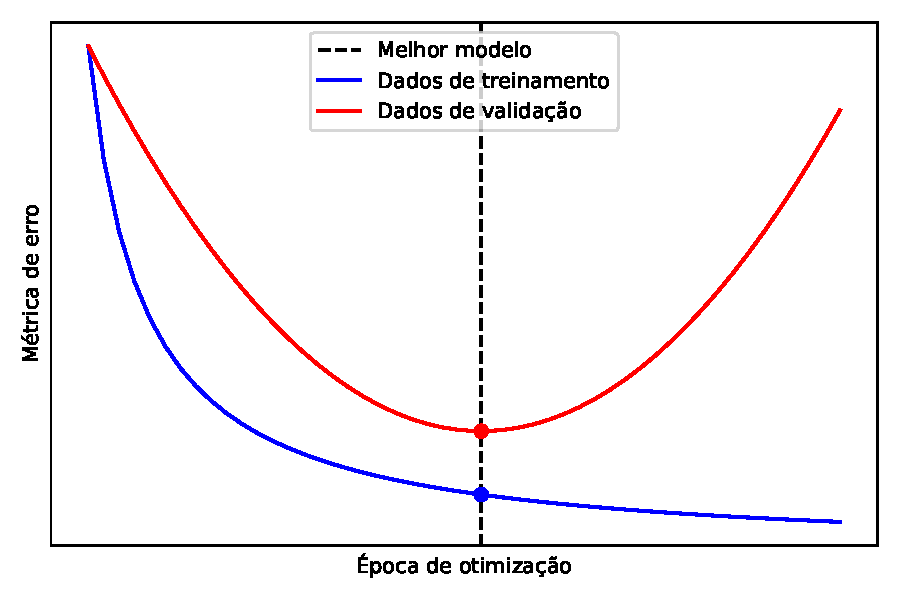
\includegraphics[width=0.7\textwidth]{overfit.pdf}
      \end{center}
      \caption{Curvas representam métricas de erro avaliadas sobre os dados de treinamento (em azul) e de validação (em vermelho) ao longo das épocas de otimização. O melhor modelo se localiza onde a curva de validação atinge seu menor valor, ponto dado pela linha tracejada.}
      \label{f:overfit}
    \end{figure}

    A forma mais simples de interrupção precoce envolve guardar o vetor de parâmetros $\vec{p}$ que resulta na melhor métrica das últimas iterações de otimização, o qual deve ser atualizado sempre que um passo de otimização resultar na melhora histórica da métrica por um valor \DIFdelbegin \DIFdel{$\Delta \geq 0$}\DIFdelend \DIFaddbegin \DIFadd{$\Delta m_0 \geq 0$}\DIFaddend . Caso contrário, inicia-se um contador para \DIFdelbegin \DIFdel{mensurar }\DIFdelend \DIFaddbegin \DIFadd{quantificar }\DIFaddend o número de iterações desde que o melhor modelo foi conseguido. Caso este número se torne superior a um valor $I_p \geq 0$ chamado de paciência, deve-se parar a otimização e retornar os melhores parâmetros guardados como resultado do treinamento. \DIFaddbegin \DIFadd{Quanto maior o valor da paciência, maior a tolerância do treinamento ao caos da convergência estocástica. }\DIFaddend Com este processo, reduzimos a possibilidade de descarte de um modelo quando \DIFaddbegin \DIFadd{isto }\DIFaddend não \DIFdelbegin \DIFdel{há necessidade}\DIFdelend \DIFaddbegin \DIFadd{é necessário}\DIFaddend .


\chapter{Cálculo do gradiente} \label{c:gradiente_calculo}

  Até o momento, sabemos construir uma função custo $C(\vec{p})$ para treinar um modelo (Seção \ref{s:objetivo}), bem como melhorá-lo a partir dela e de métodos de otimização local baseados em gradiente (Seção \ref{s:metodos_gradiente}). Neste capítulo serão discutidas as maneiras pelas quais estes gradientes podem ser calculados, incluindo considerações teóricas e práticas.

  De forma introdutória, o gradiente de uma função real $f$ em $\vec{p} \in \mathcal{R}^S$, notado por $\vec{\nabla} f(\vec{p})$, é definido matematicamente pelo vetor de derivadas parciais desta função em relação a $\vec{p}$:

  \begin{equation} \label{e:gradiente_definicao}
    \nabla f(\vec{p}) =
    \dfrac{\partial f}{\partial \vec{p}} =
    \begin{bmatrix}
      \frac{\partial f}{\partial p_1}(\vec{p}) \\
      \vdots \\
      \frac{\partial f}{\partial p_s}(\vec{p}) \\
      \vdots \\
      \frac{\partial f}{\partial p_S}(\vec{p})
    \end{bmatrix}
    .
  \end{equation}

  \noindent Por sua vez, suas derivadas parciais são calculadas a partir do limites como:

  \begin{equation} \label{e:parcial_definicao}
    \frac{\partial f}{\partial p_s}(\vec{p}) =
      \lim_{h \to 0} \frac{
        f(\vec{p} + h \vec{e}_s) - f(\vec{p})
      }{h}
      ,
  \end{equation}

  \noindent onde $h \in \mathcal{R}$ e $\vec{e}_s$ é o vetor unitário positivo que aponta na direção da dimensão $s$ de $\mathcal{R}^S$.

  Quando a função diferenciada passa a ser vetorial, $\vec{f} \in \mathcal{R}^Q$, faz mais sentido falar no termo matriz jacobiana (ou simplesmente jacobiana), que agrupa em linhas as transpostas dos gradientes de cada elemento de $\vec{f}$, notada por $J_{\vec{f}}(\vec{p})$:

  \begin{equation} \label{e:del_definicao}
    J_{\vec{f}}(\vec{p}) =
      \dfrac{\partial \vec{f}}{\partial\vec{p}} =
      \begin{bmatrix}
        \dfrac{\partial \vec{f}}{\partial p_1} & \cdots & \dfrac{\partial \vec{f}}{\partial p_s} & \cdots & \dfrac{\partial \vec{f}}{\partial p_S}
      \end{bmatrix} =
      \begin{bmatrix}
        \vec{\nabla}^\top f_1(\vec{p}) \\
        \vdots \\
        \vec{\nabla}^\top f_q(\vec{p}) \\
        \vdots \\
        \vec{\nabla}^\top f_Q(\vec{p}) \\
      \end{bmatrix}
      ,
  \end{equation}

  \noindent ou de forma explícita:

    \begin{equation} \label{e:jacobiana_definicao_explicita}
      J_{\vec{f}}(\vec{p}) =
      \begin{bmatrix}
        \frac{\partial f_1}{\partial p_1}(\vec{p}) & \cdots & \frac{\partial f_1}{\partial p_s}(\vec{p}) & \cdots & \frac{\partial f_1}{\partial p_S}(\vec{p}) \\
        \vdots& \ddots& \vdots &\iddots &\vdots  \\
        \frac{\partial f_q}{\partial p_1}(\vec{p}) & \cdots & \frac{\partial f_q}{\partial p_s}(\vec{p}) & \cdots & \frac{\partial f_q}{\partial p_S}(\vec{p}) \\
        \vdots& \iddots& \vdots &\ddots &\vdots  \\
        \frac{\partial f_Q}{\partial p_1}(\vec{p}) & \cdots & \frac{\partial f_Q}{\partial p_s}(\vec{p}) & \cdots & \frac{\partial f_Q}{\partial p_S}(\vec{p}) \\
      \end{bmatrix}
    \end{equation}

  Desta forma, a jacobiana de uma função real é a transposta de seu gradiente. A montagem computacional da jacobiana, de modo geral, exige estratégias como as que serão alvo das seções a seguir.

  \section{Diferenciação manual}

    O método de diferenciação manual é o método básico de diferenciação. Assumindo que $\vec{f}$ é diferenciável em um domínio $\mathcal{D} \subset \mathcal{R}^S$, utiliza-se a definição de limite e suas propriedades para compor a função jacobiana, que leva cada elemento $\vec{p}$ em $\mathcal{D}$ a $J_{\vec{f}}(\vec{p})$. A principal vantagem deste método é que uma vez que se possua a função jacobiana, pode-se estimar matrizes jacobianas em qualquer ponto em $\mathcal{D}$ de forma exata e eficiente. Por outro lado, a diferenciação manual exige que se possua uma equação em fórmula fechada, isto é, que as operações sejam as funções básicas da matemática e que estas sejam finitas em número. Para além destas limitações, existem funções muito difíceis ou até mesmo impossíveis de ser diferenciadas dadas as tecnologias matemáticas atuais. Outro ponto bastante negativo do método é a inescalabilidade computacional: a cada novo problema a ser diferenciado, alguém deve dedicar um possivelmente grande intervalo na formulação da função jacobiana, para só então computar seus resultados.

  \section{Diferenciação simbólica}

    A diferenciação \DIFdelbegin \DIFdel{simbólia }\DIFdelend \DIFaddbegin \DIFadd{simbólica }\DIFaddend consiste em representar, em linguagem computacional, conceitos abstratos como o de símbolos e expressões matemáticas, de forma que a manipulação dos mesmos possa resultar na \DIFdelbegin \DIFdel{resolução de problemas }\DIFdelend \DIFaddbegin \DIFadd{solução de problemas diferenciais }\DIFaddend de forma exata \DIFaddbegin \shortcite{pavelle1981computer}\DIFaddend . Por meio da computação simbólica, pode-se representar uma função de forma fechada $\vec{f}(\vec{p})$ como uma expressão matemática e utilizar da manipulação simbólica automatizada para calcular a expressão que representa a função jacobiana dentro do domínio \DIFdelbegin \DIFdel{trabalhado}\DIFdelend \DIFaddbegin \DIFadd{desejado}\DIFaddend . Este método supera a diferenciação manual, uma vez que pode produzir soluções complicadas em pouco tempo, além de ser facilmente aplicado a outros problemas realizando o mesmo processo. Entretanto, como dito, o método é limitado a expressões fechadas, o que muitas vezes não é o caso.

  \section{Diferenciação numérica} \label{s:diferenciacao_numerica}

    A diferenciação numérica diverge das técnicas manual e simbólica por não buscar respostas exatas, mas aproximações. Para tal, cada derivada parcial da matriz jacobiana é aproximada para no ponto de aplicação $\vec{p}$ de interesse. No caso do método das diferenças finitas, as derivadas parciais da forma explicitada na equação (\ref{e:parcial_definicao}) são aproximadas por:

    \begin{equation} \label{e:parcial_aproximada_diff_finitas}
      \frac{\partial \vec{f}}{\partial p_s}(\vec{p})
      =
      \lim_{h \to 0} \frac{\vec{f}(\vec{p} + h \vec{e_s}) - \vec{f}(\vec{p})}{h}
      \approx
      \frac{\vec{f}(\vec{p} + h \vec{e_s}) - \vec{f}(\vec{p})}{h}
    \end{equation}

    \noindent onde $h$ na aproximação deixa de ser uma quantidade infinitesimal para um se tornar um número muito pequeno (\textit{i.e.}, $h=0,01$).

    A vantagem da diferenciação numérica é que ela é generalizável a qualquer expressão, mesmo que ela não seja de forma fechada. A principal desvantagem é que para calcular cada derivada, deve-se aplicar a função $\vec{f}$ uma vez durante a variação de cada um dos $S$ parâmetros de $\vec{p}$. Desta maneira, se $\vec{p}$ represente uma malha de propriedades físicas de dimensão $n_x\times n_y = 1000 \times 1000 = 1.000.000$, serão necessários um milhão de aplicações diretas de $\vec{f}$ além de sua aplicação em $\vec{p}$, para o cálculo da jacbiana, o que a depender da operação realizada (\textit{i.e.}, simulação física) pode se tornar inviável. Assim, a diferenciação numérica é de aplicação geral, mas ineficiente.

  \section{Diferenciação automática (autodiff)}

    % autodiff

    A diferenciação automática (AD), também referida como autodiferenciação ou simplesmente autodiff, consegue um grande número de troféus dentre os métodos de diferenciação descritos neste capítulo. Seus resultados são exatos, eficientes, não exigem forma fechada da função a ser diferenciada, e uma vez implementada, é de aplicação a qualquer outro problema \shortcite{baydin2018automatic}. Sua desvantagem é não necessariamente produzir uma função fechada como resultado, o que é um problema apenas se a manipulação simbólica da matriz jacobiana é desejada. Neste caso, se a função utilizada tiver uma forma fechada, o tratamento simbólico sobre seu gráfico é capaz de gerar as derivadas parciais em forma fechada (\textit{i.e.}, é o caso realizado no Apêndice \ref{a:equivalencia_fwi_rnn}). Este esquema de diferenciação é generalizadamente utilizado no treinamento de modelos de aprendizado de máquina, principalmente no caso das redes neurais artificiais.

    O coração da autodiff é a ideia de que todas as computações feitas são compostas de operações mais básicas, as quais conhecemos as regras de derivação \shortcite{deisenroth2020mathematics}. Assim, conhecendo o grafo que leva as entradas às saídas de uma função genérica $\vec{f}(\vec{p})$ pode-se calcular suas derivadas por simples aplicação da regra da cadeia. Esta pode ser realizada em concordância com a ordem de execução do grafo que liga $\vec{p}$ a $\vec{f}(\vec{p})$, o que define a diferenciação automática direta, ou no sentido oposto, partindo das saídas de $\vec{f}(\vec{p})$ às suas entradas, $\vec{p}$. Este último método é denominado diferenciação automática reversa \shortcite{baydin2018automatic}.

    Algumas ideias comuns aos dois métodos de diferenciação automática são as seguintes:
    \begin{enumerate}
      \item A maior parte das computações pode ser escrita como um grafo que liga variáveis por meio de composições de operações mais básicas e com derivadas bem conhecidas.
      \item Ao invés de números, o fluxo pelo grafo de qualquer computação é realizado por meio de pares de valores primários e diferenciais --- sejam tangentes ou adjuntos.
      \item \DIFdelbegin \DIFdel{Aariáveis }\DIFdelend \DIFaddbegin \DIFadd{Variáveis }\DIFaddend e constantes só diferem por as últimas serem inicializadas com diferenciais nulas no antes da diferenciação (a segunda etapa, no caso da diferenciação reversa).
      \item A diferenciação parcial com relação a uma variável envolve tornar as outras variáveis do problema constantes (tornar suas diferenciais nulas).
    \end{enumerate}

    \subsection{Diferenciação automática direta}

      Considere a seguinte função:

      \begin{equation} \label{e:autodiff_direta_exemplo}
        \vec{f}(\vec{p}) = \vec{f}\left(
        \begin{bmatrix}
          p_1 \\
          p_2 \\
        \end{bmatrix}
        \right) =
        \begin{bmatrix}
          p_2 + p_1 p_2 \\
          \sin(p_2) \\
        \end{bmatrix} =
        \begin{bmatrix}
          f_1(\vec{p}) \\
          f_2(\vec{p}) \\
        \end{bmatrix}
        .
      \end{equation}

      \noindent O grafo de $\vec{f}(\vec{p})$ é desenhado na Figura \ref{f:autodiff_funcao}. \DIFaddbegin \DIFadd{Nela, cada círculo representa um nó, com uma variável composta por uma dupla de valores primário e tangente --- por simplicidade, apenas o valor primário está sendo representado. As setas indicam que $v_3$ pode ser calculado apenas com o conhecimento de $v_1$ e $v_2$ por meio da operação produto. Estes, por sua vez, dependem ou não das entradas $\vec{p}$ da função $\vec{f}$.
}\DIFaddend 

      \begin{figure}
        \begin{center}
          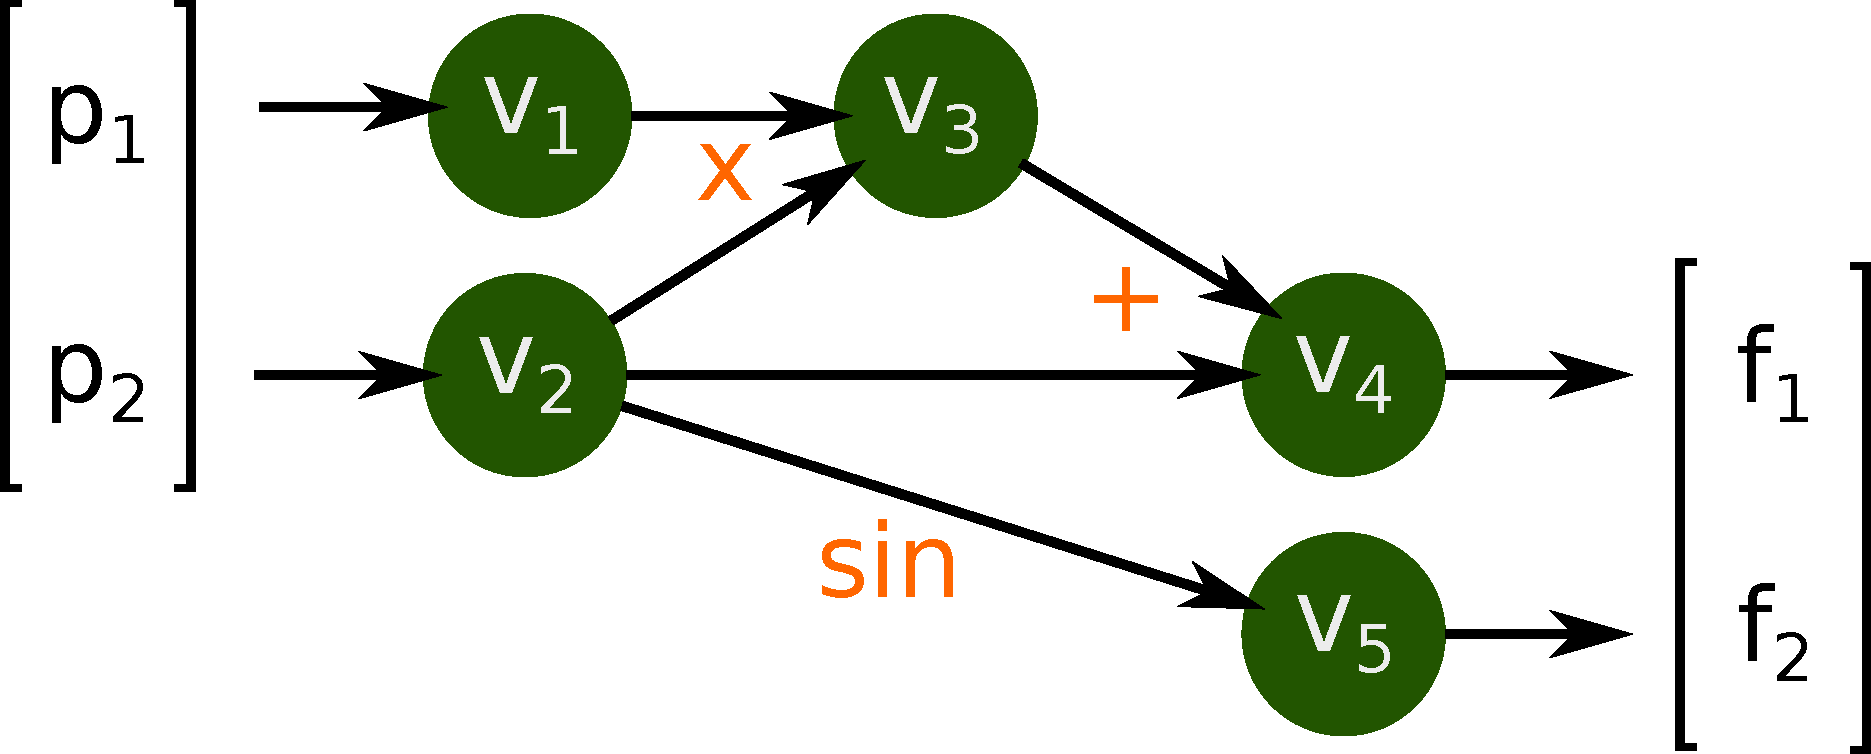
\includegraphics[width=0.6\textwidth]{autodiff_funcao.pdf}
        \end{center}
        \caption{Grafo da função $\vec{f}(\vec{p}) = \left[(p_2 + p_1 p_2)\ (\sin{p_2})\right]^\top = \left[f_1\ f_2\right]^\top$.}
        \label{f:autodiff_funcao}
      \end{figure}

      \DIFdelbegin \DIFdel{Na autodiff direta, considera-se que as variáveis são compostas de valores primários e tangentes. }\DIFdelend As tangentes são as diferenciais parciais de cada nó do grafo de $\vec{f}$ em relação à entrada à qual se deseja diferenciar, obtidas pela aplicação da regra da cadeia. \DIFaddbegin \DIFadd{A regra da cadeia é sempre calculada em partes na diferenciação automática, e é aí que mora sua capacidade de diferenciar com exatidão algoritmos complicados. }\DIFaddend Assim, caso desejemos diferenciar $f(\vec{p})$ em relação a $p_1$ no ponto $\vec{p} = [2\ 2]^\top$ por autodiff \DIFaddbegin \DIFadd{direta}\DIFaddend , devemos percorrer o grafo na Figura \ref{f:autodiff_funcao} em seu sentido natural, enquanto calculamos os valores primários e tangentes associados a cada nó até as saídas da função $\vec{f}$. As tangentes \DIFaddbegin \DIFadd{de cada nó }\DIFaddend são \DIFdelbegin \DIFdel{conseguidas }\DIFdelend \DIFaddbegin \DIFadd{calculadas }\DIFaddend por aplicação da regra da cadeia \DIFdelbegin \DIFdel{a cada ponto. Portanto, o }\DIFdelend \DIFaddbegin \DIFadd{em relação aos seus nós de dependência direta, e estes resultados são acumulados para o cálculo dos nós seguintes. Vale definir a tangente do }\DIFaddend nó $v_i$\DIFdelbegin \DIFdel{tem sua tangente }\DIFdelend \DIFaddbegin \DIFadd{, $\dot{v}_i$, como a diferencial de $v_i$ }\DIFaddend em relação à entrada $p_s$\DIFdelbegin \DIFdel{calculada por aplicação da regra da cadeia sobre:
      }\DIFdelend \DIFaddbegin \DIFadd{:
      }\DIFaddend \begin{equation} \label{e:autodiff_direta_tangente}
        \dot{v}_i = \frac{\partial v_i}{\partial p_s}
        \DIFdelbegin \DIFdel{.
      }\DIFdelend \DIFaddbegin \DIFadd{,
      }\DIFaddend \end{equation}

      \DIFaddbegin \noindent \DIFadd{onde $\dot{v}_i$ é calculada sobre as diferenciais acumuladas nos nós passados. }\DIFaddend Por exemplo, para calcularmos $\dot{v}_3$ \DIFaddbegin \DIFadd{quando diferenciamos }\DIFaddend em relação \DIFdelbegin \DIFdel{a }\DIFdelend \DIFaddbegin \DIFadd{à entrada }\DIFaddend $p_1$\DIFdelbegin \DIFdel{no grafo da Figura \ref{f:autodiff_funcao}}\DIFdelend , \DIFaddbegin \DIFadd{não precisaremos explicitar toda a expressão $v_3$, mas escrever sua derivada em função de suas dependências bem como suas respectivas tangentes. Por regra da cadeia, }\DIFaddend fazemos:
      \begin{equation} \label{e:autodiff_direta_tangente_exemplo}
        \dot{v}_3 \DIFdelbegin \DIFdel{=
        }\DIFdelend \DIFaddbegin \DIFadd{\equiv
        }\DIFaddend \frac{\partial v_3}{\partial p_1} =
        \frac{\partial v_3}{\partial p_1} v_2
          + v_1 \frac{\partial v_2}{\partial p_1} =
        \dot{v}_1 v_2 + v_1 \dot{v}_2
        ,
      \end{equation}

      \noindent onde $\dot{v}_1$ é $\frac{\partial v_1}{\partial p_1} = 1$, pois $v_1 = p_1$, e $\dot{v}_2 = \frac{\partial v_2}{\partial p_1} = 0$, pois $v_2$ não depende de $p_1$. Todos os passos \DIFdelbegin \DIFdel{deste exemplo }\DIFdelend \DIFaddbegin \DIFadd{da autodiferenciação direta do grafo em discussão }\DIFaddend são descritos, \DIFdelbegin \DIFdel{tanto com relação aos primários, quanto com relação às tangentes, }\DIFdelend na Tabela \ref{t:autodiff_direta_exemplo}, onde os nós são calculados por ordem de necessidade. Como realizado aqui, a ideia da diferenciação automática é calcular a derivada parcial passo a passo, por aplicação recorrente da regra da cadeia, enquanto se resolve o cálculo direto da função. Neste método, as tangentes dos últimos nós compõem exatamente as colunas da matriz jacobiana de $\vec{f}(\vec{p})$ de número igual ao número do parâmetro ao qual $\vec{f}$ foi diferenciada.

      A implementação da autodiff direta geralmente inclui uma estrutura de dados capaz de armazenar os dois valores, o primário e a tangente, e a definição de todas as operações básicas em conjunto com suas regras de derivação. Assim, a função de multiplicação entre duas variáveis deve ser implementada de forma a não só multiplicar os primários das duas entradas, como somar as multiplicações entre o primário de uma entrada e a tangente da outra (regra da derivada do produto). Daí em frente, sempre que a multiplicação entre dois valores for realizada, a propagação das tangentes também o será.

      Um exemplo de implementação da diferenciação automática direta escrito em Python está presente no Apêndice \ref{a:autodiff_direta} deste documento.

      \begin{table}[]
        \centering
        \begin{tabular}{@{}cllll@{}}
          \toprule
          \textbf{Passo} & \multicolumn{2}{c}{\textbf{Primários}}  & \multicolumn{2}{c}{\textbf{Tangentes}}                        \\  \midrule
            & \multicolumn{2}{c}{\color{gray} \footnotesize Nós de entrada}                    & \multicolumn{2}{c}{\color{gray} \footnotesize Nós de entrada}                                               \\
          {\color{gray} 1}     & $v_1 = p_1$                       & $=2$              & $\dot{v}_1 = \frac{\partial v_1}{\partial p_1}$             & $=1$       \\
          {\color{gray} 2}     & $v_2 = p_2$                       & $=2$              & $\dot{v}_2 = \frac{\partial v_2}{\partial p_1}$             & $=0$       \\
            & \multicolumn{2}{c}{\color{gray} \footnotesize Nós intermediários}                    & \multicolumn{2}{c}{\color{gray} \footnotesize Nós intermediários}                                               \\
          {\color{gray} 3}     & $v_3 = v_1 v_2$                   & $=4$                & $\dot{v}_3 = \dot{v}_1 v_2 + \dot{v}_2 v_1$                 & $= 2+0= 2$ \\
          {\color{gray} 4}     & $v_4 = v_2 + v_3$                 & $=6$                & $\dot{v}_4 = \dot{v}_2 + \dot{v}_3$                         & $=2$       \\
          {\color{gray} 5}     & $v_5 = sin(v_2)$                  & $=0.91\ldots$       & $\dot{v}_5 = 0$                                             & $= 0$      \\
            & \multicolumn{2}{c}{\color{gray} \footnotesize Nós de saída}                    & \multicolumn{2}{c}{\color{gray} \footnotesize Nós de saída}                                               \\
          {\color{gray} 6}     & $f_1 = v_4$            & $=6$               & $\frac{\partial f_1}{\partial p_1} = \dot{f}_1 = \dot{v}_4$ & $\boldsymbol{=2}$       \\
          {\color{gray} 7}     & $f_2 = v_5$   & $=0.91\ldots$               & $\frac{\partial f_2}{\partial p_1} = \dot{f}_2 = \dot{v}_5$ & $\boldsymbol{=0}$      \\ \bottomrule
        \end{tabular}
        \caption{Processo de diferenciação automática direta da função $\vec{f}$ em relação ao seu primeiro parâmetro, $p_1$ no ponto $\vec{p} = [2\ 2]^\top$.}
        \label{t:autodiff_direta_exemplo}
      \end{table}

      Por completude, a multiplicação da matriz jacobiana por um vetor à direita é muito comum em problemas de otimização (\textit{i.e.}, pelo vetor de resíduos: $J_{\vec{f}}\ \vec{r}$) e é geralmente custosa. Este procedimento pode ser realizado sem necessidade de construir a matriz jacobiana usando tecnologia de autodiferenciação. Para isso, os nós de entrada recebem como primários os valores do ponto em que se deseja calcular o jacobiano, enquanto suas tangentes são tomadas como o vetor ao qual se deseja multiplicar, $\vec{r}$. As tangentes finais deste processo são $J_{\vec{f}}\ \vec{r}$ \shortcite{baydin2018automatic}.

      A autodiferenciação direta é muito eficiente quando se possui poucas entradas e muitas saídas. De outro modo, a autodiferenciação reversa é vantajosa. Este método será descrito na seção a seguir.

    \subsection{Diferenciação automática reversa}

      Na diferenciação automática reversa, tenta-se calcular a regra da cadeia no sentido oposto do grafo. O modo reverso é um pouco mais capcioso que o direto, uma vez que nele se deseja derivar o resultado que ainda não foi calculado com relação aos valores intermediários, e finalmente, os de entrada da função. Por isso, ao invés de uma única passada pelo grafo da função, a autodiff reversa exige duas. A primeira calcula os primários e mapeia as operações e dependências ocorridas no grafo, enquanto a segunda ocorre no sentido oposto, uma vez que o grafo já é conhecido a esse ponto, calculando as diferenciais, por propagação reversa, das saídas às entradas.

      A autodiff reversa possui dois conceitos similares aos da direta. Ao invés de primários e tangentes, temos primários e adjuntos. Neste modelo, escolhemos uma das saídas da função $\vec{f}(\vec{p})$, $f_q$, e a diferenciamos com relação às entradas, ou seja, calcular $\vec{\nabla} f_q(\vec{p})$ --- note a semelhança com o gradiente de uma função custo, $\vec{\nabla} C(\vec{p})$. Nestes termos, o novo conceito de adjunto é definido para $v_i$ da seguinte maneira:

      \begin{equation} \label{e:autodiff_reversa_adjunto}
        \bar{v}_i = \frac{\partial f_q}{\partial v_i}
        ,
      \end{equation}

      \noindent e representa a sensibilidade da saída $f_q$ em relação a $v_i$, e deve ser calculado pela aplicação contínua da regra da cadeia em sentido reverso. Assim, para calcularmos a derivada parcial de $f_1$ em relação a $v_2$ a partir do grafo na Figura \ref{f:autodiff_funcao}, temos:

      \begin{equation} \label{e:autodiff_reversa_tangente_exemplo}
        \bar{v}_2
        =
        \frac{\partial f_1}{\partial v_4} \left(
          \frac{\partial v_4}{\partial v_3} \frac{\partial v_3}{\partial v_2} +
          \frac{\partial v_4}{\partial v_2}
        \right)
        =
        \frac{\partial f_1}{\partial v_3} \frac{\partial v_3}{\partial v_2} +
        \frac{\partial f_1}{\partial v_4} \frac{\partial v_4}{\partial v_2}
        =
        \bar{v}_3 \frac{\partial v_3}{\partial v_2} +
        \bar{v}_4 \frac{\partial v_4}{\partial v_2}
        ,
      \end{equation}

      O resultado da equação (\ref{e:autodiff_reversa_tangente_exemplo}) é composto naturalmente durante diferenciação reversa, onde múltiplas contribuições a um mesmo nó são somadas, como observado na Tabela \ref{t:autodiff_reversa_exemplo} durante a diferenciação de $f_1$ em relação a seus parâmetros no ponto $\vec{p} = [2\ 2]^\top$.

      Por comparação, na seção \ref{s:diferenciacao_numerica} vimos que se uma função custo $C(\vec{p})$ depende de $S=1.000.000$ parâmetros, utilizar diferenciação numérica para calcular o gradiente de $C$ em $\vec{p}$ implicaria no cálculo direto de $C$ um milhão e uma de vezes; por autodiferenciação direta, o número de operações necessárias seria de um milhão; já por autodiferenciação reversa conseguimos resultados expressivamente superiores em casos como este: apenas duas operações são necessárias para calcular todo o gradiente de $C$ em relação a $\vec{p}$. De forma mais genérica, temos por garantia que, se $\vec{f}$ é um mapeamento $\mathcal{R}^S \longrightarrow \mathcal{R}^Q$, utilizar diferenciação reversa é mais vantajoso se $Q\ll S$. Um detalhe importante, é que a complexidade extra causada pelo cálculo de uma função dentro de um esquema de diferenciação automática é garantida de ser de um fator menor que 6, tipicamente se enquadrando entre 2 e 3.

      A implementação deste método exige mais cuidado, pois é necessária a construção de alguma estrutura para guardar todas as informações sobre estrutura do grafo, o que torna este tipo de diferenciação custosa em uso de memória. Assim como na implementação do modo direto, também aqui é necessário definir todas as operações básicas juntamente às suas regras de diferenciação, além da forma de guardar estas informações na estrutura de grafo utilizada, de maneira que seja possível realizar o segundo passe diferenciando pelo grafo. Um exemplo de esquema de diferenciação automática reversa escrito implementado na linguagem Python se encontra no Apêndice \ref{a:autodiff_direta} deste material.

      \begin{table}[]
        \centering
        \begin{tabular}{@{}cllcll@{}}
          \toprule
          \textbf{Passo} & \multicolumn{2}{c}{\textbf{Primários}}                 & \textbf{ Passo} & \multicolumn{2}{c}{\textbf{Adjuntos}}                                        \\ \midrule
                & \multicolumn{2}{c}{\color{gray} \footnotesize Nós de entrada}              &       & \multicolumn{2}{c}{\color{gray} \footnotesize Nós de entrada}                                  \\
          {\color{gray} 1}     & $v_1 = p_1$                     & $=2$          & {\color{gray} 15}    & $\frac{\partial f_1}{\partial p_1} = \bar{v}_1$ & $\boldsymbol{=2}$              \\
          {\color{gray} 2}     & $v_2 = p_2$                     & $=2$          & {\color{gray} 14}    & $\frac{\partial f_1}{\partial p_2} = \bar{v}_2$ & $\boldsymbol{=3}$     \\
          {\color{gray}  }     & \multicolumn{2}{c}{\color{gray} \footnotesize Nós intermediários}            &       & \multicolumn{2}{c}{\color{gray} \footnotesize Nós intermediários}                              \\
          {\color{gray} 3}     & $v_3 = v_1 v_2$                 & $=4$           & {\color{gray} 13}    & $\bar{v}_1 = v_2 \bar{v}_3$                     & $=2 \times 1=2$   \\
          {\color{gray} 4}     & $v_4 = v_2 + v_3$               & $=6$          & {\color{gray} 12}    & $\bar{v}_2 = \bar{v}_2 + v_1 \bar{v}_3$         & $=1+2 \times 1=3$ \\
          {\color{gray} 5}     & $v_5 = \sin(v_2)$               & $=0.91\ldots$ & {\color{gray} 11}    & $\bar{v}_3 = \bar{v}_4$                       & $=1$              \\
          {\color{gray}  }     &                                 &               & {\color{gray} 10}    & $\bar{v}_2 = \bar{v}_4$                       & $=1$              \\
          {\color{gray}  }     & \multicolumn{2}{c}{\color{gray} \footnotesize Nós de saída}                             &       & \multicolumn{2}{c}{\color{gray} \footnotesize Nós de saída}                              \\
          {\color{gray} 6}     & $f_1 = v_4$          & $=6$          & {\color{gray} 9}     & $\bar{v}_4 = \frac{\partial f_1}{\partial v_4}$ & $=1$              \\
          {\color{gray} 7}     & $f_2 = v_5$ & $=0.91\ldots$ & {\color{gray} 8}     & $\bar{v}_5 = \frac{\partial f_1}{\partial v_5}$ & $=0$              \\ \bottomrule
        \end{tabular}
        \caption{Processo de diferenciação automática reversa da primeira saída da função $\vec{f}$, $f_1$, em relação aos seus parâmetros no ponto $\vec{p} = [2\ 2]^\top$.}
        \label{t:autodiff_reversa_exemplo}
      \end{table}

      De forma similar à autodiferenciação direta, onde as tangentes no fim do processo representam uma coluna da matriz jacobiana, os adjuntos no final da diferenciação reversa representam uma de suas linhas (a linha referente à dimensão parcialmente diferenciada). Este método também é útil no cálculo da multiplicação pela transposta da jacobiana, $\vec{J}_{\vec{f}}^\top \vec{r}$. Para tal, de modo semelhante à autodiff direta, os valores adjuntos que inicializam a segunda etapa da diferenciação reversa devem ser inicializados com os valores de $\vec{r}$. Desta forma, as tangente obtidas ao fim do processo são o resultado da multiplicação, sem a necessidade de construir toda a matriz jacobiana antes do resultado.

      As características dos métodos de diferenciação discutidas nesta seção são sumarizadas na Tabela \ref{t:metodos_diferenciacao_caracteristicas}.

      \begin{table}[]
        \centering
        \begin{tabular}{@{}ccccl@{}}
          \multicolumn{4}{c}{Método de diferenciação}                                    &                                  \\
          \textbf{Manual} & \textbf{Simbólica} & \textbf{Numérica} & \textbf{Automática} & Característica                   \\
          \checkmark      & \checkmark         & -                 & \checkmark          & \textbf{Exata}                   \\
          \checkmark      & \checkmark         & -                 & \checkmark          & \textbf{Computacionalmente eficiente}               \\
          -               & \checkmark         & \checkmark        & \checkmark          & \textbf{Generalizável}          \\
          -               & -                  & \checkmark        & \checkmark          & \textbf{Não exige forma fechada de $\vec{f}$} \\
          \checkmark      & \checkmark         & -                 & \checkmark\textsuperscript{$\ast$} & \textbf{Retorna forma fechada de $J_{\vec{f}}$}               \\
        \end{tabular}
        \caption{Características dos métodos de diferenciação. ($\ast$): Caso a função estudada seja dada em forma fechada e um tratamento simbólico for dado ao grafo.}
        \label{t:metodos_diferenciacao_caracteristicas}
      \end{table}


\chapter{De regressões lineares a redes neurais}

  As redes neurais artificiais (ANNs) formam uma imensa contribuição tecnológica ao mundo moderno. Esta classe de modelos com estrutura arbitrária é altamente versátil, sendo capaz de produzir resultados no estado-da-arte nas áreas de previsão temporal, filtragem de sinais, segmentação de imagens, aproximação de funções, análise de sentimento, produção automática de música, reconhecimento de voz, tradução e muito mais. É possível enxergar no percurso histórico na criação destes modelos um caminho que segue naturalmente dos problemas de regressão linear ao seu estado atual. Este capítulo visa evidenciar tal percurso a partir da matemática.

  \section{Regressão linear} \label{s:reg_linear}

    O método da regressão linear é um modelo estatístico bastante simples e com propriedades profundamente conhecidas. A técnica é considerada um dos primeiros métodos de aprendizado de máquina existentes. \DIFdelbegin \DIFdel{Dado um }\DIFdelend \DIFaddbegin \DIFadd{Considerando uma amostra $\vec{x}$, o modelo, $\vec{f}$, consiste em sua combinação linear com uma matriz de pesos, $\boldsymbol{W}$, de forma a gerar um vetor $\vec{\hat{y}}$ de predições:
}

    \begin{equation} \DIFadd{\label{e:reg_linear_amostra}
      \vec{\hat{y}} = \vec{f}(\vec{x}) = \boldsymbol{W} \vec{x}
      .
    }\end{equation}

    \noindent \DIFadd{Um esquema deste modelo pode ser visto na Figura \ref{f:regressao_linear}.
}

    \begin{figure}
      \begin{center}
        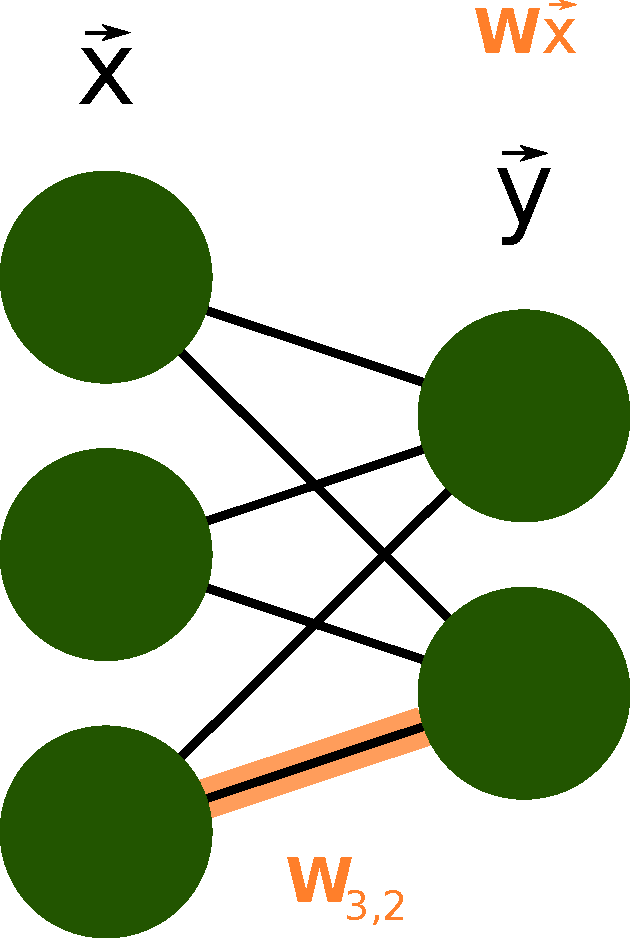
\includegraphics[width=0.2\textwidth]{regressao_linear.pdf}
      \end{center}
      \caption{\DIFaddFL{Grafo de um modelo de regressão linear com três entradas e duas saídas.}}
      \label{f:regressao_linear}
    \end{figure}

    \DIFadd{Para generalizar o modelo a um }\DIFaddend conjunto de observações, $\boldsymbol{X}_{N\times M}$, \DIFdelbegin \DIFdel{e }\DIFdelend \DIFaddbegin \DIFadd{tendo-se em vista um conjunto }\DIFaddend de efeitos alvos \DIFaddbegin \DIFadd{a elas }\DIFaddend associados, $\boldsymbol{Y}_{N\times Q}$, pode-se desenvolver um modelo linear $f$ tal que $f(\boldsymbol{X}) = \boldsymbol{\hat{Y}}_{N\times Q} \approx \boldsymbol{Y}_{N\times Q}$ para regredir $\boldsymbol{Y}_{N\times Q}$ a partir de $\boldsymbol{X}_{N\times M}$ \DIFdelbegin \DIFdel{linearmente }\DIFdelend da seguinte maneira:

    \begin{equation} \label{e:reg_linear}
      f(\boldsymbol{X}) = \boldsymbol{X} \boldsymbol{W}
      ,
    \end{equation}

    \noindent onde $\boldsymbol{W}_{M\times Q}$ é a matriz de parâmetros que possui em cada coluna $m$ as relações lineares das colunas de $\boldsymbol{X}$ e a coluna $m$ de $\boldsymbol{Y}$. Quando $M=Q=1$, diz-se que a regressão é simples, isto é, uma variável de entrada está sendo relacionada a uma única variável de saída; quando $Q = 1$ e $M > 1$, trata-se de uma regressão multi-variável, uma vez que cada observação consta de $M$ variáveis, as quais se relacionam com uma única variável de saída; e quando $M,Q>1$, trata-se de um modelo linear geral, que associa $M$ variáveis a $Q$ outras variáveis. Este último, porém, pode ser escrito como uma composição de $Q$ modelos lineares multivariáveis que são independentes entre si \shortcite{kim2006univariate}.

    Quando treinado diretamente sobre os dados, um modelo com a forma da equação (\ref{e:reg_linear}) possui viés, uma vez que este não considera efeitos em $\boldsymbol{Y}$ que são independentes das variáveis utilizadas na regressão. Em outras palavras, ele parte do princípio de que se as variáveis de entrada são nulas, as saídas também serão nulas. Para atenuar este viés, deve-se adicionar uma variável auxiliar de valor fixo e independente das observações reais\DIFdelbegin \DIFdel{, tipicamente de valor }\DIFdelend \DIFaddbegin \DIFadd{. A adição desta variável independente toma a forma de $\vec{b}$ na equação a seguir:
}

    \begin{equation} \DIFadd{\label{e:reg_linear_amostra_b}
      \vec{\hat{y}} = \vec{f}(\vec{x}) = \boldsymbol{W} \vec{x} + \vec{b}
      .
    }\end{equation}


    \DIFadd{Já para várias amostras, uma variável vetorial cujos elementos possuem um mesmo valor --- tipicamente }\DIFaddend unitário \DIFdelbegin \DIFdel{, }\DIFdelend \DIFaddbegin \DIFadd{($\vec{1}$) --- é adicionada }\DIFaddend à esquerda de $\boldsymbol{X}$, formando a matrix de observações estendida, $\boldsymbol{X}'$. Nestes termos, a matriz de parâmetros $\boldsymbol{W}$, que multiplica $\boldsymbol{X}'$ à direita, deve pertencer a $\mathcal{R}^{(M+1) \times Q}$:

    \begin{equation} \label{e:reg_linear_W}
      \boldsymbol{W} =
      \begin{bmatrix}
        \vec{w}_{0}^\top \\
        \vec{w}_{1}^\top \\
        \vdots \\
        \vec{w}_{m}^\top \\
        \vdots \\
        \vec{w}_{M}^\top \\
      \end{bmatrix} =
      \begin{bmatrix}
        w_{01} & \cdots & w_{0q} & \cdots & w_{0Q} \\
        w_{11} & \cdots & w_{1q} & \cdots & w_{1Q} \\
        \vdots & & \vdots & & \vdots\\
        w_{m1} & \cdots & w_{mq} & \cdots & w_{mQ} \\
        \vdots & & \vdots & & \vdots\\
        w_{M1} & \cdots & w_{Mq} & \cdots & w_{MQ} \\
      \end{bmatrix}
      ,
    \end{equation}

    \noindent e o modelo em (\ref{e:reg_linear_desenviesado}) se torna desenviesado, uma vez que a primeira linha de $\boldsymbol{W}$, $\vec{w}_0^\top$, que não multiplica as reais variáveis observadas, $\boldsymbol{X}$, é treinada para obter valores que balanceiem o viés do modelo linear. $\vec{w}_0^\top$ recebe os nomes de \emph{termo independente}, \emph{valor de interceptação} e, no contexto das redes neurais, de \emph{viés}.

    \begin{equation} \label{e:reg_linear_desenviesado}
      f(\boldsymbol{X}) = \begin{bmatrix} \vec{1} & \boldsymbol{X} \end{bmatrix} \boldsymbol{W}
      ,
    \end{equation}

    Existem diversas técnicas para inverter este modelo e descobrir os valores dos parâmetros em $\boldsymbol{W}$ (\textit{i.e.}, $\boldsymbol{W}=(\boldsymbol{X}^\top \boldsymbol{X})^{-1}\boldsymbol{X}^\top \boldsymbol{Y}$ para um problema sobredeterminado \shortcite{deisenroth2020mathematics}). Utilizando os conceitos deste material, podemos criar uma função custo $C(\boldsymbol{W})$ adequada (\textit{i.e.}, $C(\boldsymbol{W}) = MSE(f(\boldsymbol{X}), \boldsymbol{Y})$), e treiná-lo com base em um dos métodos gradiente citados (\textit{i.e.}, SGD).

    A interpretação de $\boldsymbol{W}$ é profundamente compreendida \shortcite{james2013introduction}. A partir de seus valores pode-se retirar informações quantitativas e qualitativas sobre as relações entre as variáveis observadas e as alvejadas. Primeiramente cada um dos $Q$ elementos em $\vec{w}_0$ afirma sobre o que ocorre com as respectivas $Q$ saídas do modelo quando todas as variáveis são nulas, uma espécie de ponto inicial do modelo $f$. Para $m>0$, os $Q$ elementos de $\vec{w}_m$ são relacionados à importância das variáveis observadas para a predição das $Q$ saídas. Valores pequenos implicam em baixa correlação entre as variáveis relacionadas, enquanto valores muito positivos implicam em forte correlação linear entre as variáveis. Por outro lado, valores muito negativos implicam em uma relação inversa entre as variáveis observada e alvo analisadas. Diretamente, o valor $w_{m,q}$ explica o incremento sobre a saída $q$ do modelo quando a variável observada $m$ aumenta de uma unidade. Uso destes modelos pode, por exemplo, justificar, para uma empresa, o aumento de verba destinada a publicidade, caso o modelo linear treinado explique o número de vendas realizadas a partir desta variável por meio de um parâmetro $w$ positivo.

  \section{Regressão logística}

    \DIFdelbegin \DIFdel{A apesar }\DIFdelend \DIFaddbegin \DIFadd{Apesar }\DIFaddend do nome de regressão, a regressão logística é um modelo de classificação. \DIFdelbegin \DIFdel{Este }\DIFdelend \DIFaddbegin \DIFadd{A história deste método é bem desenvolvida por }\shortciteN{cramer2002origins}\DIFadd{. Tal }\DIFaddend modelo se estende da regressão linear para calcular probabilidades de uma determinada amostra com $M$ dimensões (ou $M$ variáveis) pertencer a cada uma das $Q$ classes consideradas. Um exemplo simples é o cálculo da probabilidade de um cliente com determinada quantidade de recursos ser confiável a empréstimos bancários --- em outras palavras, a probabilidade de o cliente fazer parte da categoria de clientes confiáveis em detrimento da classe de clientes não-confiáveis.

    O modelo de regressão logística é definido de forma muito similar ao da regressão linear. Considera-se que as probabilidades reais de pertencimento de cada amostra de treinamento nas linhas da matriz de observações $\boldsymbol{X}$ a cada uma das $Q>1$ classes é dada nas linhas da matriz $\boldsymbol{Y}$\footnote{No caso da classificação, $\boldsymbol{Y}$ é típicamente construída a partir da transformação \textit{one-hot} dos rótulos das amostras às quais se sabe a classificação. Ver Apêndice \ref{a:one_hot}.}. Nestes termos, um modelo de regressão logística é descrito por $f(\boldsymbol{X}) = \boldsymbol{\hat{Y}} \approx \boldsymbol{Y}$, \DIFdelbegin \DIFdel{onde:
}\DIFdelend \DIFaddbegin \DIFadd{como na equação (\ref{e:reg_logistica}). O grafo deste modelo para uma amostra pode ser visto na Figura \ref{f:regressao_logistica} e deve ser comparado ao da regressão linear na Figura \ref{f:regressao_linear}.
}\DIFaddend 

    \DIFaddbegin \begin{figure}
      \begin{center}
        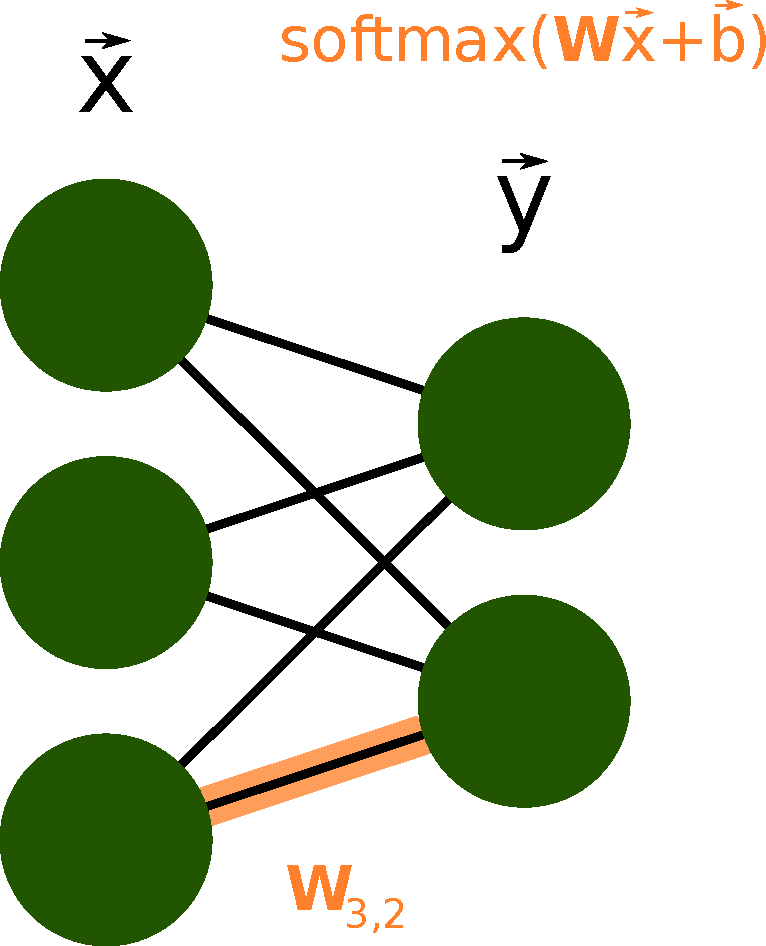
\includegraphics[width=0.2\textwidth]{regressao_logistica.pdf}
      \end{center}
      \caption{\DIFaddFL{Grafo de um modelo de regressão logística multinomial com três entradas e duas saídas probabilísticas.}}
      \label{f:regressao_logistica}
    \end{figure}

    \DIFaddend \begin{equation} \label{e:reg_logistica}
      f(\boldsymbol{X}) = \text{softmax}\left(\boldsymbol{X} \boldsymbol{W}\right)
    \DIFdelbegin \DIFdel{.
    }\DIFdelend \end{equation}

    \noindent Aqui, a função de normalização exponencial é notada por $\text{softmax}$, e funciona como um normalizador de probabilidades, sendo aplicada a cada linha da matriz resultante de $\boldsymbol{X}\boldsymbol{W}$. Assim, as saídas desta combinação linear, cujos valores pertencem ao intervalo $[-\infty,+\infty]$, são comprimidas ao intervalo de probabilidades válidas: $[0,1]$. Além disso, esta função garante que o somatório das probabilidades de pertencimento de uma mesma amostra às classes possíveis seja sempre igual a 1 (100\%). Matematicamente, a função $\text{softmax}$ é definida para um vetor $\vec{z}$ da seguinte maneira:

    \begin{equation} \label{e:softmax}
      \text{softmax}(\vec{z}) =
      \frac{e^{\vec{z}}}{\vec{1}^\top e^{\vec{z}}} =
      \frac{e^{\vec{z}}}{\sum_{q=1}^Q e^{z_q}}
      , \qquad \vec{z} \in \mathcal{R}^Q
      .
    \end{equation}

    A regressão logística é dita binomial quando o número de classses $Q$ é igual a 2, e multinomial quando $Q>2$. Mostra-se que uma regressão logística multinomial com $Q$ classes pode ser escrita a partir de $Q-1$ regressões binomiais, uma vez que sabendo-se de $Q-1$ probabilidades de classificação, a desconhecida deve somar 100\% com as primeiras. Isto significa que para o caso binomial basta que uma das probabilidades seja conhecida para se determinar a outra. Este artifício pode ser implementada por meio da investigação da função softmax quando $Q=2$:

    \begin{equation} \label{e:softmax_binomial}
      \text{softmax}(\vec{z}) =
      %\frac{e^{\begin{bmatrix} z_1 \\ z_2 \end{bmatrix}}}{e^{z_1} + e^{z_2}} =
      \begin{bmatrix}
        \frac{e^{z_1}}{e^{z_1} + e^{z_2}} \\
        \frac{e^{z_2}}{e^{z_1} + e^{z_2}}
      \end{bmatrix} =
      \begin{bmatrix}
        \frac{1}{1 + e^{-(z_1-z_2)}} \\
        \frac{1}{1 + e^{z_1-z_2}}
      \end{bmatrix} =
      \begin{bmatrix}
        \frac{1}{1 + e^{-z_\star}} \\
        \frac{1}{1 + e^{z_\star}}
      \end{bmatrix} =
      \begin{bmatrix}
        \sigma(z_\star) \\
        \sigma(-z_\star) \\
      \end{bmatrix}, \qquad z_\star = z_1-z_2
      ,
    \end{equation}

    \noindent onde $\sigma$ é a função sigmoide descrita por:

    \begin{equation} \label{e:sigmoid}
      \sigma(z) = \frac{1}{1+e^{-z}}
      .
    \end{equation}

    \noindent Em nosso contexto, $\vec{z}^\top$ deve ser lido como uma das linhas da combinação linear $\boldsymbol{X}\boldsymbol{W}$ na equação (\ref{e:reg_logistica}). Por fim, a probabilidade das amostras em $\boldsymbol{X}$ pertencerem à primeira classe de em uma regressão logística binomial é descrita por:

    \begin{equation} \label{e:reg_logistica_binomial}
      f(\boldsymbol{X}) = \sigma \left( \boldsymbol{X} \vec{w} \right)
      .
    \end{equation}

    \noindent onde $w \in \mathcal{R}^{M}$ é a matriz com um único vetor de parâmetros. Este tratamente implica num treinamento eficiente, uma vez que o modelo de uma única probabilidade só depende de $M$ parâmetros. Em comparação, o tratamento multinomial padrão exigiria $2M$ parâmetros em $W$ ($M$ deles para cada uma das $Q=2$ classes).

    \DIFdelbegin %DIFDELCMD < \noindent %%%
\DIFdelend O gráfico \DIFdelbegin \DIFdel{desta }\DIFdelend \DIFaddbegin \DIFadd{da }\DIFaddend função \DIFaddbegin \DIFadd{sigmoide }\DIFaddend (Figura \ref{f:sigmoid}) demonstra de forma visual sua não-linearidade\DIFaddbegin \DIFadd{, }\DIFaddend e portanto a não-linearidade inerente à função $\text{softmax}$.

    \begin{figure}
      \begin{center}
        \DIFdelbeginFL %DIFDELCMD < 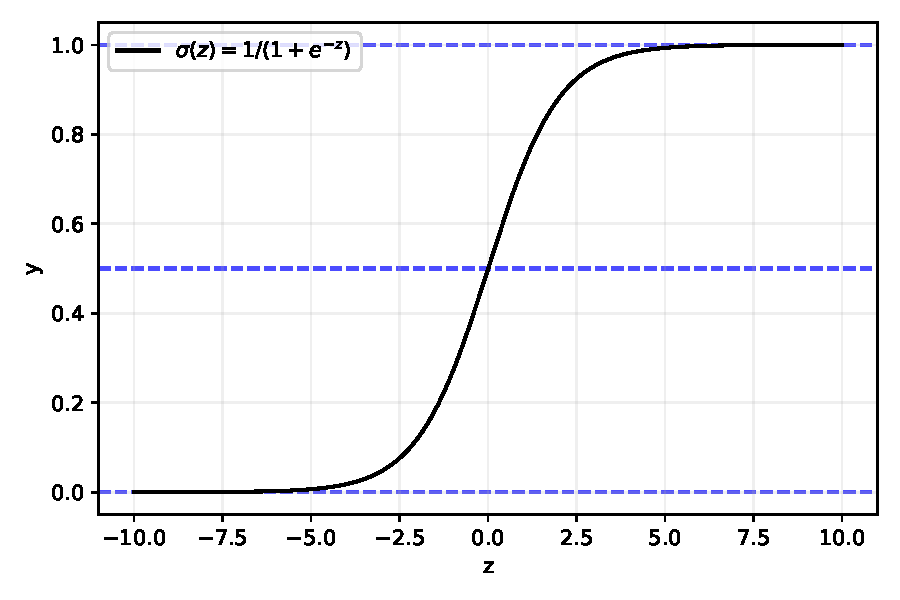
\includegraphics[width=0.8\textwidth]{sigmoid.pdf}
%DIFDELCMD <       %%%
\DIFdelendFL \DIFaddbeginFL 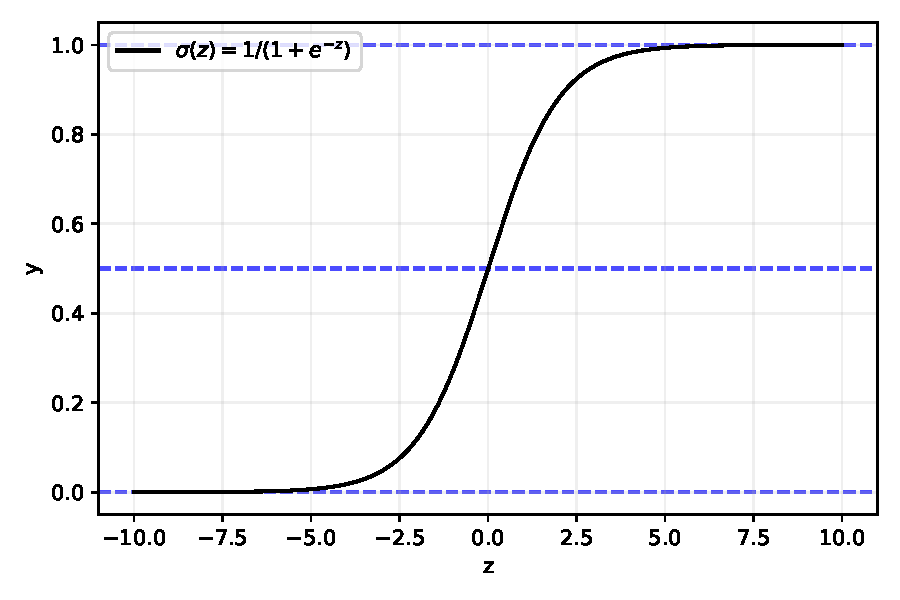
\includegraphics[width=0.6\textwidth]{sigmoid.pdf}
      \DIFaddendFL \end{center}
      \caption{Gráfico da função sigmoide ($\sigma(z) = \frac{1}{1+e^{-z}}$)}
      \label{f:sigmoid}
    \end{figure}

    Assim como no caso da regressão linear, por padrão o modelo logístico é enviesado por assumir que uma amostra nula possui probabilidade $1/Q$ de pertencer a cada uma de suas $Q$ classes. A remoção deste viés ocorre da mesma forma que a demonstrada na Seção \ref{s:reg_linear}: adicionamos uma coluna extra com valor unitário ao início da matriz de observações $\boldsymbol{X}$, de forma que a primeira linha de $\boldsymbol{W}$ contenha os parâmetros que balancearão o viés do modelo para cada classe. Portanto, o modelo de regressão logística multinomial desenviesado é descrito na equação (\ref{e:reg_logistica_desenviesado}):

    \begin{equation} \label{e:reg_logistica_desenviesado}
      f(\boldsymbol{X}) =
      \text{softmax}\left(
        \begin{bmatrix}
          \vec{1} & \boldsymbol{X}
        \end{bmatrix} \boldsymbol{W}
        \right)
      ,
    \end{equation}

    \noindent enquanto o modelo de regressão logística binomial desenviesado é dado na equação (\ref{e:reg_logistica_binomial_desenviesado})

    \begin{equation} \label{e:reg_logistica_binomial_desenviesado}
      f(\boldsymbol{X}) =
      \sigma\left(
        \begin{bmatrix}
          \vec{1} & \boldsymbol{X}
        \end{bmatrix} \vec{w}
        \right)
    \end{equation}

    A rotulação de cada amostra é dada então pela classe de maior probabilidade calculada. A interpretação destes modelos também foi fortemente estudada, e segue similar ao caso da regressão linear, exceto que o elemento $w_{m,q}$ da matriz $\boldsymbol{W}$ afirma sobre o incremento de probabilidade de uma amostra à classe $q$ dado um determinado incremento sobre a variável $m$ monotonicamente, entretanto não-linear. \DIFaddbegin \shortciteN{menard2001applied} \DIFadd{descreve o processo de interpretação de modelos logísticos de forma detalhada, bem como suas propriedades essenciais.
}\DIFaddend 

    Uma forma para inverter modelos de classificação para descobrir os valores dos parâmetros em $\boldsymbol{W}$ é definir uma função custo $C(\boldsymbol{W})$ adequada, por exemplo a entropia cruzada média, e buscar seu mínimo por meio de um dos métodos gradiente aqui descritos (\textit{i.e.}, Adam).

  \section{Redes neurais artificiais}

    Em \citeyearNP{mcculloch1943logical}, o neurofisiologista Warren McCulloch e o lógico Walter Pitts publicam um artigo explicando o funcionamento do sistema nervoso. Sua descrição é especial na história da ciência por seu empenho em formalizar o comportamento biológico dos neurônios. É sabido da biologia que um neurônio pode ser dividido em duas partes: soma e axônio. A soma se refere ao corpo celular de um neurônio, enquanto o axônio é sua parte mais alongada, funcionando como um transmissor de sinais gerados na soma a outros neurônios ou tecidos.

    \begin{figure}
      \begin{center}
        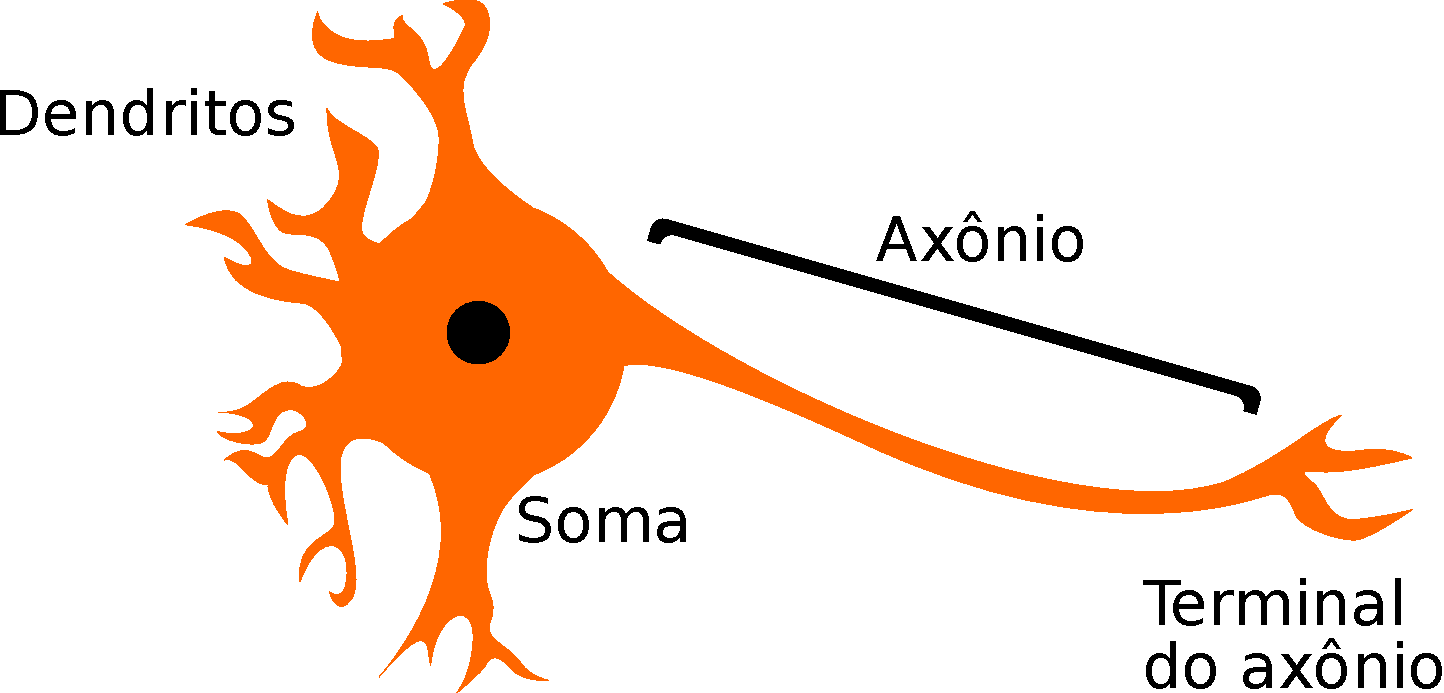
\includegraphics[width=0.5\textwidth]{neuronio_biologico.pdf}
      \end{center}
      \caption{Estrutura básica de um neurônio.}
      \label{f:neuronio_biologico}
    \end{figure}

    Quando é estimulado com intensidade suficiente para ser excitado, isto é, com uma diferença de potencial superior a um valor limiar (seu potencial de ação), ele é completamente ativado, propagando um pulso elétrico à frente. O intervalo até a inicialização da resposta elétrica é determinado pelo próprio neurônio, entretanto a amplitudade do sinal é sempre fixa. Este princípio é chamado ``princípio do tudo ou nada da atividade nervosa''. Após transitar pelo axônio, o sinal emitido pela soma é capturado por outro neurônio em regiôes conhecidas como sinapses, e um conjunto de neurônios conectados entre si, por vezes chamado de rede neural. Rede, não linha, pois não é comum que um neurônio seja ativado pelo impulso elétrico gerado por um único vizinho. Em geral a excitação de um neurônio ocorre quando uma célula neural é estimulada por múltiplos vizinhos dentro de frações de milisegundo. Por fim, a velocidade de propagação elétrica nas porções mais longas dos axônios é alta, da ordem de $150$ m/s, de forma que é razoável considerar que pulsos que saem de uma mesma fonte chegam instantaneamente em seus destinos, independentemente da distância percorrida.

    McCulloch e Pitts nos propõem que tal comportamento definido no princípio do tudo ou nada, onde a resposta de um neurônio é binária (sem sinal ou pulso definido) é tratável em termos de lógica proposicional. Assim, a atividade de cada neurônio pode ser representada como uma proposição que é calculada sobre os pulsos previamente recebidos. A representação matemática inicialmente proposta em seu trabalho, bem como suas incontáveis variações recentes, é atualmente conhecida pelo termo geral ``rede neural artificial'' (\textit{artificial neural network} -- ANN).

    Os primeiros trabalhos envolvendo ANNs foram justificados como uma tentativa de melhor entender o funcionamento do cérebro, desde a biofísica matemática de \shortciteN{rashevsky1938contribution}, por meio de seu modelamento matemático. \shortciteN{rummelhart1986parallel} mostraram então que utilizar propagação reversa --- um caso especial da diferenciação automática reversa para quando se possui uma única variável de saída (\textit{i.e.}, função objetivo) ---, torna possivel o treinar modelos de rede neural parametrizados matematicamente, e que estes poderiam resultar em aplicações interessantes. Somente em \citeyearNP{lecun1989backpropagation}, \shortciteANP{lecun1989backpropagation} demonstraram um uso prático de treinamento de rede para a comunidade científica. Seu resultado foi um programa de computador capaz de reconhecer dígitos em códigos de barras por meio de uma rede neural convolucional. A introdução de placas gráficas para o treinamento de redes profundas foi fortemente evidenciada como um avanço tecnológico útil ao assunto por meio do trabalho de \shortciteN{ciresan2011flexible}. Dez anos depois, as redes neurais são estudadas como modelos preditores versáteis e eficientes, sendo aplicadas em virtualmente todas as áreas da ciência, direta ou indiretamente afetando a vida de todos os seres humanos.

    Em especial, no que tange a este trabalho, o artigo de \shortciteN{mcculloch1943logical} divide-as em dois tipos: livres de círculos e com presença de círculos. Estes dois casos são respectivamente tratados hoje pelos termos "rede neural pró-alimentada" (\textit{feed-forward neural network} -- FNN) e "rede neural retro-alimentada" (\textit{recurrent neural networks} -- RNN), as quais serão tratadas nas subseções a seguir.

    \subsection{Redes neurais pré-alimentadas (FNN)} \label{s:fnn}

      O perceptron \shortcite{rosenblatt1958perceptron} é considerado o primeiro modelo de rede neural artifical inventado. Com as conexões corretas, este algoritmo pode desempenhar uma classificação binária. Sua formulação matemática para classificar uma matriz de amostras $\boldsymbol{X}$ é dada por:

    \begin{equation} \label{e:perceptron_original}
      f(\boldsymbol{X}) = \text{H}\left( \begin{bmatrix} \vec{1} & \boldsymbol{X}\end{bmatrix} \vec{w} \right)
      ,
    \end{equation}

    \noindent onde $H$ é a função degrau de Heaviside, utilizada como função de ativação para o neurônio de saída, e $\vec{w}$ são os pesos do modelo:

    \begin{equation} \label{e:heaviside}
      H(z) = \begin{cases}
        0, & z \le 0 \\
        1, & z > 0
      \end{cases}
      .
    \end{equation}

    É perceptível a semelhança entre o perceptron e a regressão logística binomial desenviesada --- equação (\ref{e:reg_logistica_binomial_desenviesado}), onde ao invés da função degrau, utiliza-se a função sigmoide ($\sigma$) como função de ativação. A generalização do perceptron é a sua versão multicamadas (\textit{multilayer perceptron}, MLP). Estes modelos podem ser usados como solução para um número infinito de problemas, e podem ser pensados como o empilhamento de múltiplas regressões multinomiais com funções de ativação arbitrárias. O fato de que uma operação linear como a função identidade pode ser utilizada como função de ativação final de um MLP implica que estes modelos são úteis tanto para classificação, quanto para regressão \shortcite{murtagh2003multilayer} --- de fato, este modelo generaliza os modelos de regressão linear multivariada e logística multinomial.

    Nos termos do MLP, a regressão linear, a regressão logística e até mesmo um perceptron possuem $L=2$ camadas de neurônios: uma cujos neurônios comportam os valores de entrada, e outra cujos neurônios comportarão as saídas do modelo. Um modelo MLP possui ao menos $L=3$ camadas, sendo que cada camada $\vec{a}^{[l] \in \mathcal{R}^{n_l}}$ possui $n_l$ neurônios e é calculada com base na aplicação de uma função de ativação, $T^{[l-1]}$, sobre a combinação linear da camada anterior $\vec{a}^{[l-1]} \in \mathcal{R}^{n_{l-1}}$ com uma matriz de pesos $\boldsymbol{W}^{[l-1]} \in \mathcal{R}^{n_{l-1}\times n_l}$. Como usualmente deseja-se um modelo desenviesado, deve-se adicionar um termo que balanceie o viés em cada camada antes da ativação, o qual será notado por $\vec{b}^{[l-1]}$. Esta recursão se inicia a partir da segunda camada, uma vez que a primeira camada, $\vec{a}^{[1]}$, recebe apenas os valores de entrada, $\vec{x} \in \mathcal{R}^{M}$. Deste modo, a camada $\vec{a}^{[L]} \in \mathcal{R}^{Q}$ dá as saídas da rede\shortcite{chen2018neural,nguyen2020exploration}. Todas as camadas entre a de entrada e a de saída são chamadas de intermediárias. A Figura \ref{f:mlp} ilustra uma rede com 5 camadas, onde $\{n_l\} = \{3,4,5,3,2\}$ e $T^{[i]}=\sigma$, $i=1,\ldots,4$. Esta rede é representada pela seguinte função:

    \begin{equation} \label{e:mlp_exemplo}
      f(\vec{x}) =
      \sigma(
        \boldsymbol{W}^{[4]} \sigma(
          \boldsymbol{W}^{[3]} \sigma(
            \boldsymbol{W}^{[2]} \sigma(
              \boldsymbol{W}^{[1]}
                \vec{x}
              + {\vec{b}^{[1]}})
            + {\vec{b}^{[2]}})
          + {\vec{b}^{[3]}})
        + {\vec{b}^{[4]}})
      ,
    \end{equation}

    \noindent ou para um conjunto de observações $\boldsymbol{X}_{N\times M}$:

    \begin{equation} \label{e:mlp_exemplo_muitas_obs}
      f(\boldsymbol{X}) =
      \sigma\left(
        \begin{bmatrix} \vec{1} & \sigma\left(
          \begin{bmatrix} \vec{1} & \sigma\left(
            \begin{bmatrix} \vec{1} & \sigma\left(
              \begin{bmatrix} \vec{1} & \boldsymbol{X} \end{bmatrix}
            \boldsymbol{W}^{[1]}\right) \end{bmatrix}
          \boldsymbol{W}^{[2]}\right) \end{bmatrix}
        \boldsymbol{W}^{[3]}\right) \end{bmatrix}
      \boldsymbol{W}^{[4]}\right)
      ,
    \end{equation}

    \noindent onde o viés é solucionado como nas seções anteriores, por adição de uma coluna unitária a $\boldsymbol{X}$, de forma que a primeira linha de cada matriz de pesos $\boldsymbol{W}^{[l]}$ assume um valor para equilibrar o viés do modelo linear e $\sigma$ é aplicada elemento-a-elemento.

    \begin{figure}
      \begin{center}
        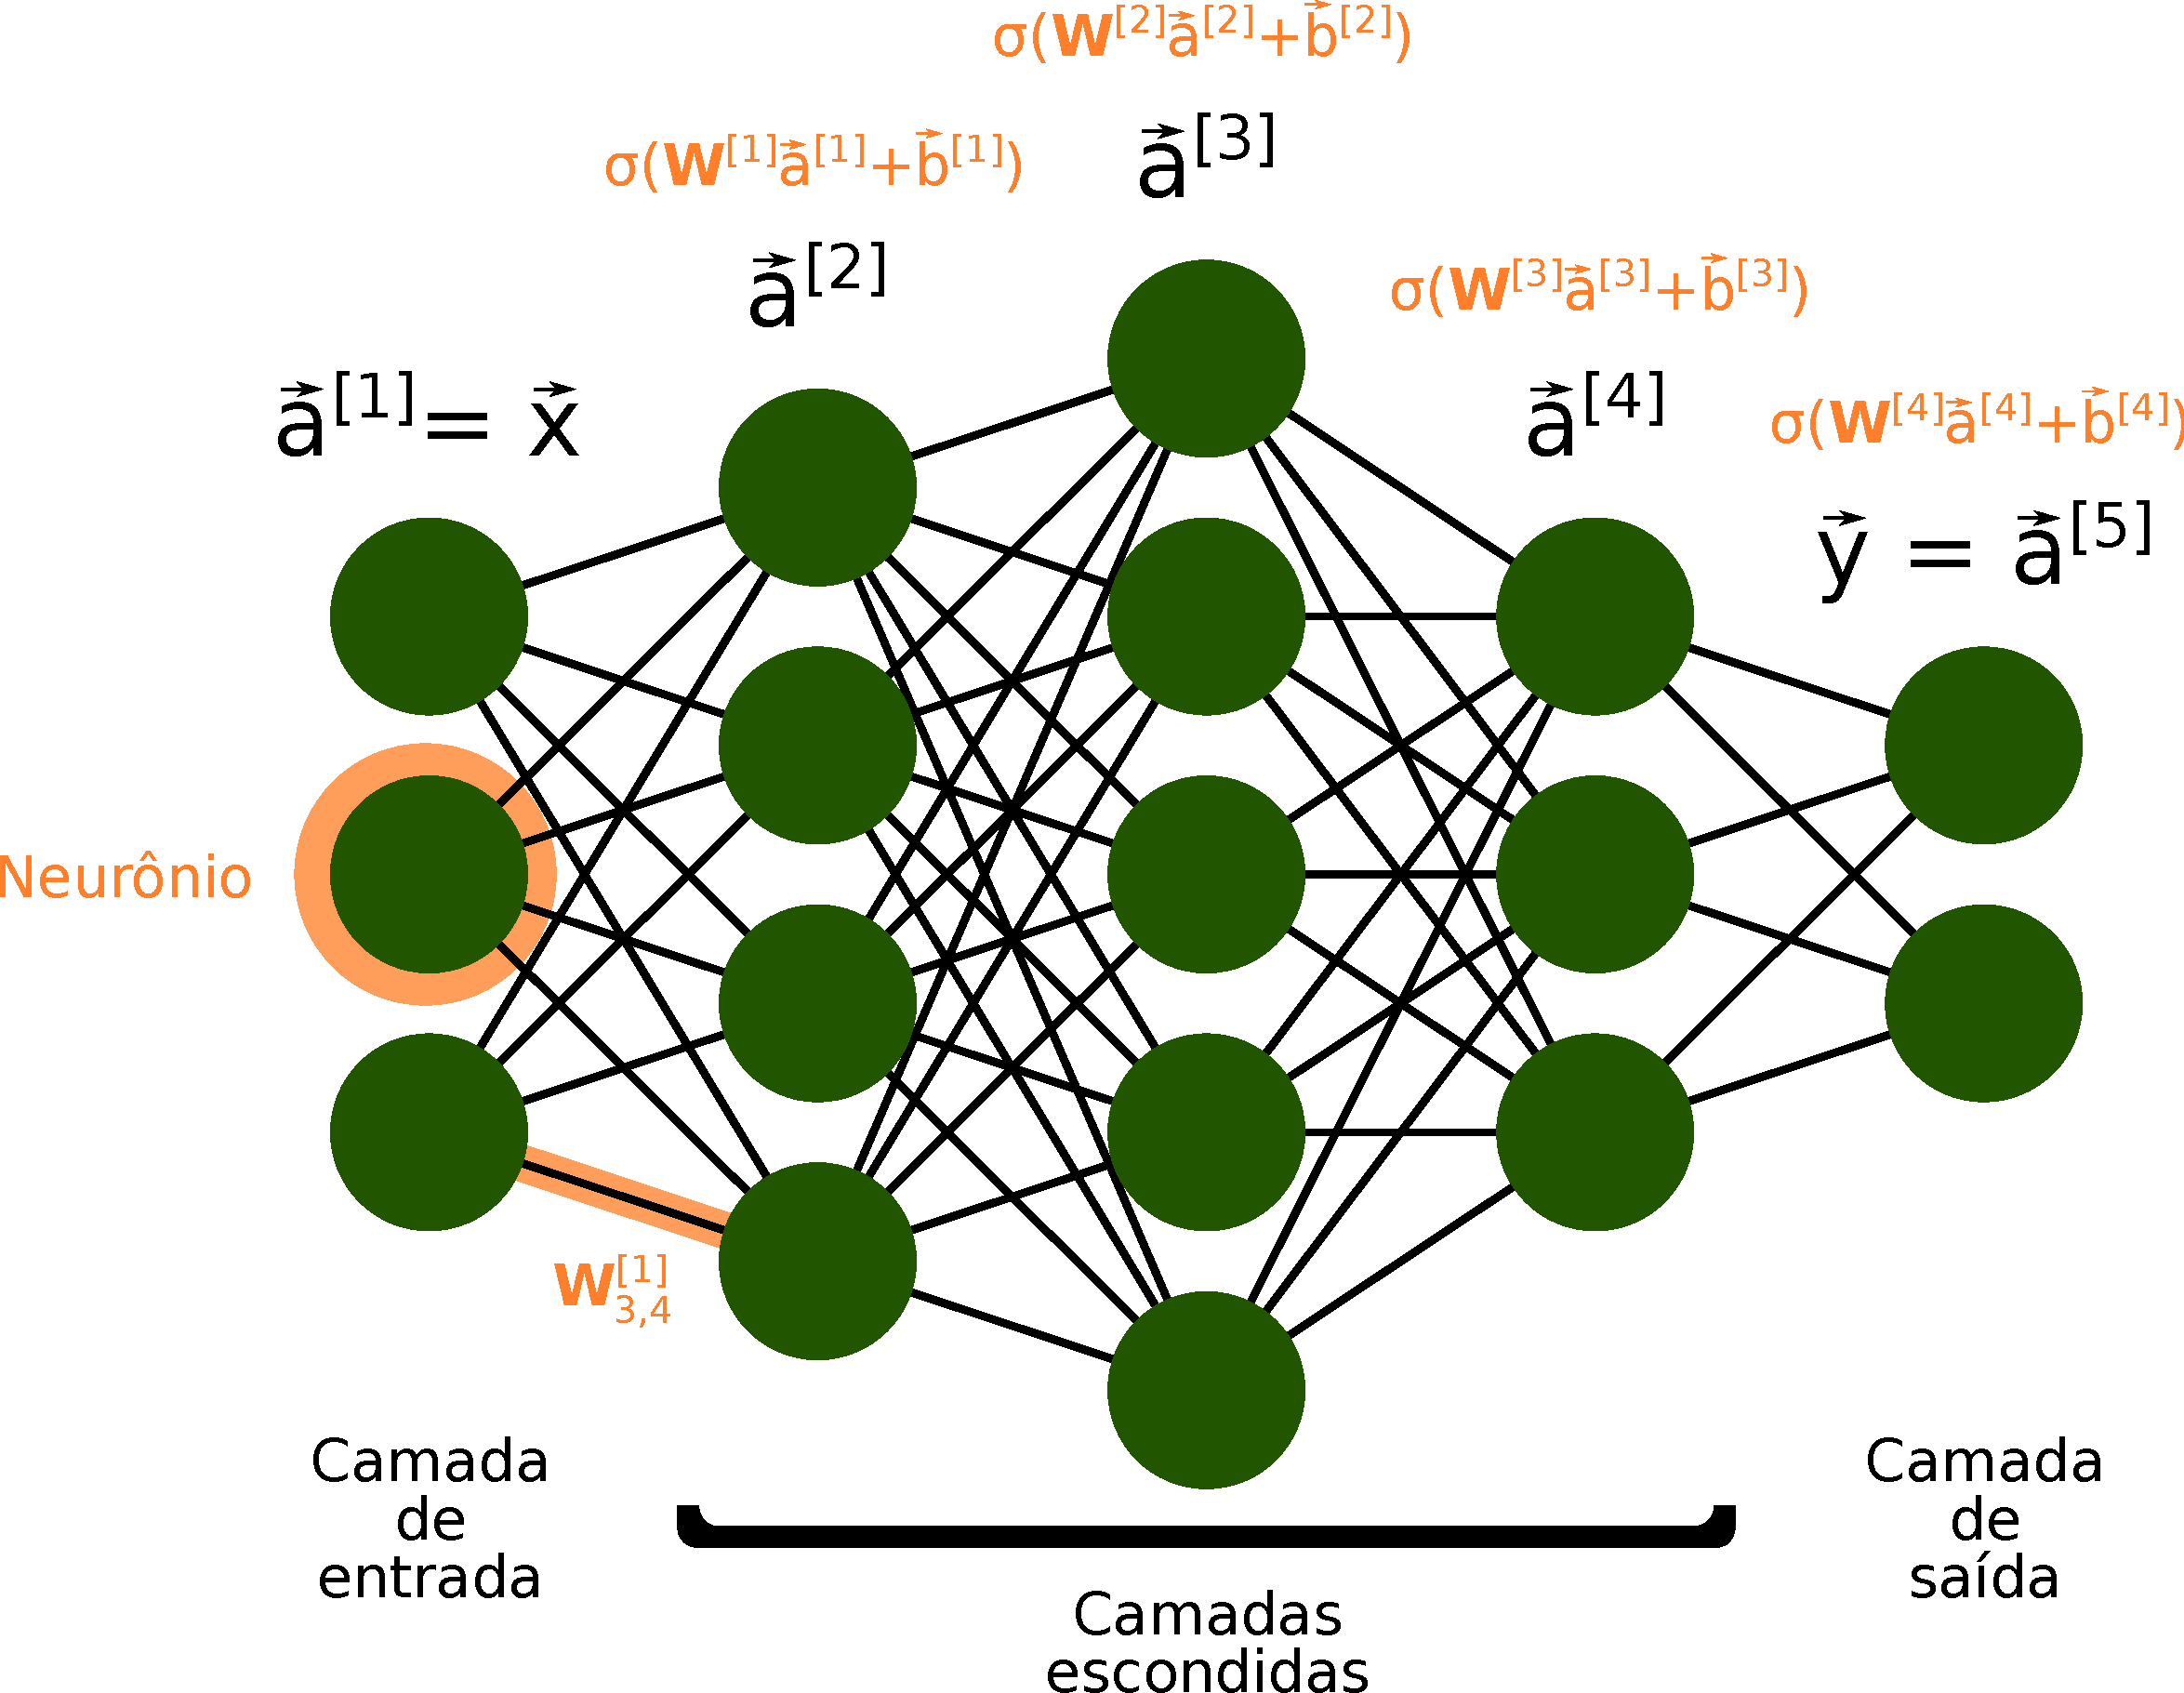
\includegraphics[width=0.9\textwidth]{mlp.pdf}
      \end{center}
      \caption{Ilustração de uma rede neural tipo MLP com \DIFdelbeginFL \DIFdelFL{sequência de }\DIFdelendFL número de camadas $L=5$ e sequência de neurônios por camada $\{n_l\} = \{3,4,5,3,2\}$. Esta rede possui entradas em $\mathcal{R}^{3}$ e saídas em $\mathcal{R}^{2}$.}
      \label{f:mlp}
    \end{figure}

    A grande vantagem dos MLPs com relação aos modelos de regressão linear é sua capacidade de prever eventos não-lineares, o que decorre diretamente do uso de funções de ativação não-lineares. Quanto mais profunda uma rede é, isto é, quanto maior seu número de camadas intermediárias, mais livre para aproximar funções não-lineares ela se torna, desde que suas camadas intermediárias sejam ativadas por funções não-lineares. Quando apenas ativações lineares são utilizadas, porém, mesmo um modelo de um milhão de camadas será sempre equivalente a um outro modelo de duas, por conta da dependência linear entre as mesmas.

    Um código para treinamento de MLPs utilizando o esquema de diferenciação automática do Apêndice \ref{a:autodiff_reversa} é provido no Apêndice \ref{a:treinamento_mlp}. O que é comum não só às redes tipo MLP como a todas as redes FNN é a ausência de conexões cíclicas para no cálculo de qualquer variável. Desta forma, elementos de uma mesma camada de neurônios não possuem dependencia. Isto não necessariamente é o caso para as redes RNN, as quais serão discutidas na subseção a seguir.

    \subsection{Redes neurais recorrentes (RNN)} \label{s:rnn}

      O modelo de rede neural pré-alimentada considera, enquanto tentativa de modelagem do sistema nervoso, que um processo de pensamento no cérebro é dependente apenas de estímulos externos. Mesmo McCulloch e Pitts \citeyear{mcculloch1943logical} tinham noção de que isto é uma aproximação, uma vez que este sistema é dotado de ligações cíclicas\footnote{Dentre outros fenômenos aqui desconsiderados, como a facilitação, a extinção e o aprendizado.}, as quais permitem que um mesmo estímulo elétrico continue reverberando dentro da rede por um longo período de tempo, interagindo multiplas vezes com um mesmo \DIFdelbegin \DIFdel{nerônio}\DIFdelend \DIFaddbegin \DIFadd{neurônio}\DIFaddend .

      De um ponto de vista mais pragmático, as redes pré-alimentadas incorrem em problemas ao representar entradas que envolvem a dimensão do tempo. A representação de séries temporais nestes modelos, apesar de tratável, é estruturalmente inadequada. Por exemplo, considere as três sequências temporais a seguir:

      \begin{enumerate} \centering
        \item $\begin{bmatrix} 0 & 0 & 1 \end{bmatrix}$;
        \item $\begin{bmatrix} 0 & 1 & 0 \end{bmatrix}$;
        \item $\begin{bmatrix} 1 & 0 & 0 \end{bmatrix}$.
      \end{enumerate}

      \noindent Tais sequências são facilmente identificadas como similares, podendo indicar o caminhar de um pulso unitário ao longo de três intervalos de tempo. Entretanto, este significado seria corrompido numa rede pré-alimentada como o perceptron, onde cada uma das sequências representariam vetores que apontam em direções completamente diferentes --- observe-as como pontos num gráfico sobre eixos cartesianos em $\mathcal{R}^3$, e enxergará estes dados da forma que uma rede neural pré-alimentada os enxerga.

      Uma solução ao problema das séries temporais é a implementação de algum sistema de memória. Tal solução já se encontrava teoricamente no artigo de \shortciteN{mcculloch1943logical}, mas sua implementação e tratamento eram inviáveis. Somente em \citeyearNP{jordan1986serial} nasce o primeiro método para se lidar com entradas sequenciais numa rede rede neural utilizando variáveis de estado. Ambos os modelos de Jordan \citeyear{jordan1986serial} e seu sucessor, o de Elman \citeyear{elman1990finding}, se baseiam na geração de uma variável de memória calculada com base em variáveis do passo temporal anterior e corrente, a qual é utilizada no cálculo das novas saídas.

      % usar o termo célula
      O modelo de Jordan utiliza como memória as saídas do último passo temporal processado ($\vec{y}_{t-1}$), que são utilizadas junto às entradas do instante atual, $\vec{x}_t$, na geração de uma variável de estado com dimensão fixa, $\vec{h}_t$, que por sua vez é utilizada no cálculo da saída atual ($\vec{y}_t$). As equações que descrevem a célula recorrente deste modelo para cada passo $t$ são dadas em (\ref{e:jordan_ht}) e (\ref{e:jordan_yt}), onde $f_h$ e $f_y$ são funções genéricas. Duas representações para a rede de Jordan podem ser vistas na Figura \ref{f:jordan}.

      \begin{equation} \label{e:jordan_ht}
        \vec{h}_t = f_h(\vec{x}_t, \vec{y}_{t-1})
      \end{equation}
      \begin{equation} \label{e:jordan_yt}
        \vec{y}_t = f_y(\vec{h}_t)
      \end{equation}

      No caso da rede de Elman, por outro lado, utiliza-se a própria memória do instante anterior, $\vec{h}_{t-1}$, para compor com $\vec{x}_t$ uma nova memória, $\vec{h}_t$, que como na rede Jordan, é utilizada na geração da saída atual ($\vec{y}_t$). As seguintes equações \DIFaddbegin \DIFadd{mostram }\DIFaddend a célula de recorrência de uma rede de Elman:

      \begin{equation} \label{e:elman_ht}
        \vec{h}_t = f_h(\vec{x}_t, \vec{h}_{t-1})
      \end{equation}
      \begin{equation} \label{e:elman_yt}
        \vec{y}_t = f_y(\vec{h}_t)
        ,
      \end{equation}

    \noindent onde $f_h$ e $f_y$ são funções genéricas. Duas representações para a rede de Elman podem ser vistas na Figura \ref{f:elman}.

      Para que as redes descritas acima sejam treináveis, é necessário que as funções $f_h$ e $f_y$ possuam parâmetros de aplicação, os quais podem ser aprendidos num processo futuro de otimização. Desta forma, tais funções são geralmente definidas como simples combinações:

      \begin{equation} \label{e:jordan_linear_part_ht}
        \vec{h}_t = \boldsymbol{W}_{hx} \vec{x}_t + \boldsymbol{W}_{hy} \vec{y}_{t-1}
      \end{equation}
      \begin{equation} \label{e:jordan_linear_part_yt}
        \vec{y}_t = \boldsymbol{W}_{yh} \vec{h}_t
        ,
      \end{equation}

      \noindent sendo cada um dos elementos dos operadores $\boldsymbol{W}_{hx}$, $\boldsymbol{W}_{hh}$ e $\boldsymbol{W}_{yh}$ os parâmetros do modelo.

      Observe que em (\ref{e:jordan_linear_part_ht}) e (\ref{e:jordan_linear_part_yt}), $\vec{y}_t$ pode ser escrita como combinação linear de $\vec{x}_t$ e $\vec{y}_{t-1}$ diretamente, sem necessidade da utilização da variável de estado $\vec{h}_t$. Durante o treinamento do modelo, tamanha linearidade logo se torna uma limitação ao aprendizado de comportamentos, pois muitos dos problemas estudados envolvem soluções que não são lineares, de forma similar ao já discutido na Seção \ref{s:fnn}. Portanto, nas redes de Jordan e Elman derivadas de operadores lineares adiciona-se um nível controlado de não-linearidade por meio da aplicação final de uma função de ativação bem conhecida, como a função sigmoide, que é definida na equação (\ref{e:sigmoid}) e pode ser vista na Figura \ref{f:sigmoid}, que comprime os resultados das combinações lineares gerando maior complexidade ao modelo. Observa-se facilmente pelo gráfico da função sigmoide, que quanto mais à esquerda de zero (abscissa da inflexão) for a entrada, mais sua imagem se aproxima de 0. Nos termos da rede neural, estímulos negativos serão suprimidos pela rede, e como a escolha do valor de corte suave igual a zero utilizado na supressão é arbitrária, a própria decisão da função de ativação introduziu um viés ao modelo.

      Para resolver o viés causado na escolha de funções de ativação, geralmente se \DIFdelbegin \DIFdel{adiona }\DIFdelend \DIFaddbegin \DIFadd{adiciona }\DIFaddend um termo de translação nas abscissas, na forma de um vetor de parâmetros extra a ser treinado, propriamente nomeado \textit{termo de viés}. As redes de Jordan e de Elman são finalmente escritas em suas formas desenviesadas mais simples nas duplas de equações (\ref{e:jordan_linear_ht}) e (\ref{e:jordan_linear_yt}), e (\ref{e:elman_linear_ht}) e (\ref{e:elman_linear_yt}), nas quais as funções de ativação escolhidas são $T_h$ e $T_y$, e os termos de viés são $\vec{b}_h$ e $\vec{b}_y$.

      \begin{equation} \label{e:jordan_linear_ht}
        \vec{h}_t = T_h(\boldsymbol{W}_{hx} \vec{x}_t + \boldsymbol{W}_{hy} \vec{y}_{t-1} + \vec{b}_h)
      \end{equation}
      \begin{equation} \label{e:jordan_linear_yt}
        \vec{y}_t = T_y(\boldsymbol{W}_{yh} \vec{h}_t + \vec{b}_y))
      \end{equation}

      \begin{equation} \label{e:elman_linear_ht}
        \vec{h}_t = T_h(\boldsymbol{W}_{hx} \vec{x}_t + \boldsymbol{W}_{hh} \vec{h}_{t-1} + \vec{b}_h)
      \end{equation}
      \begin{equation} \label{e:elman_linear_yt}
        \vec{y}_t = T_y(\boldsymbol{W}_{yh} \vec{h}_t + \vec{b}_y))
      \end{equation}

      \begin{figure}
        \begin{center}
          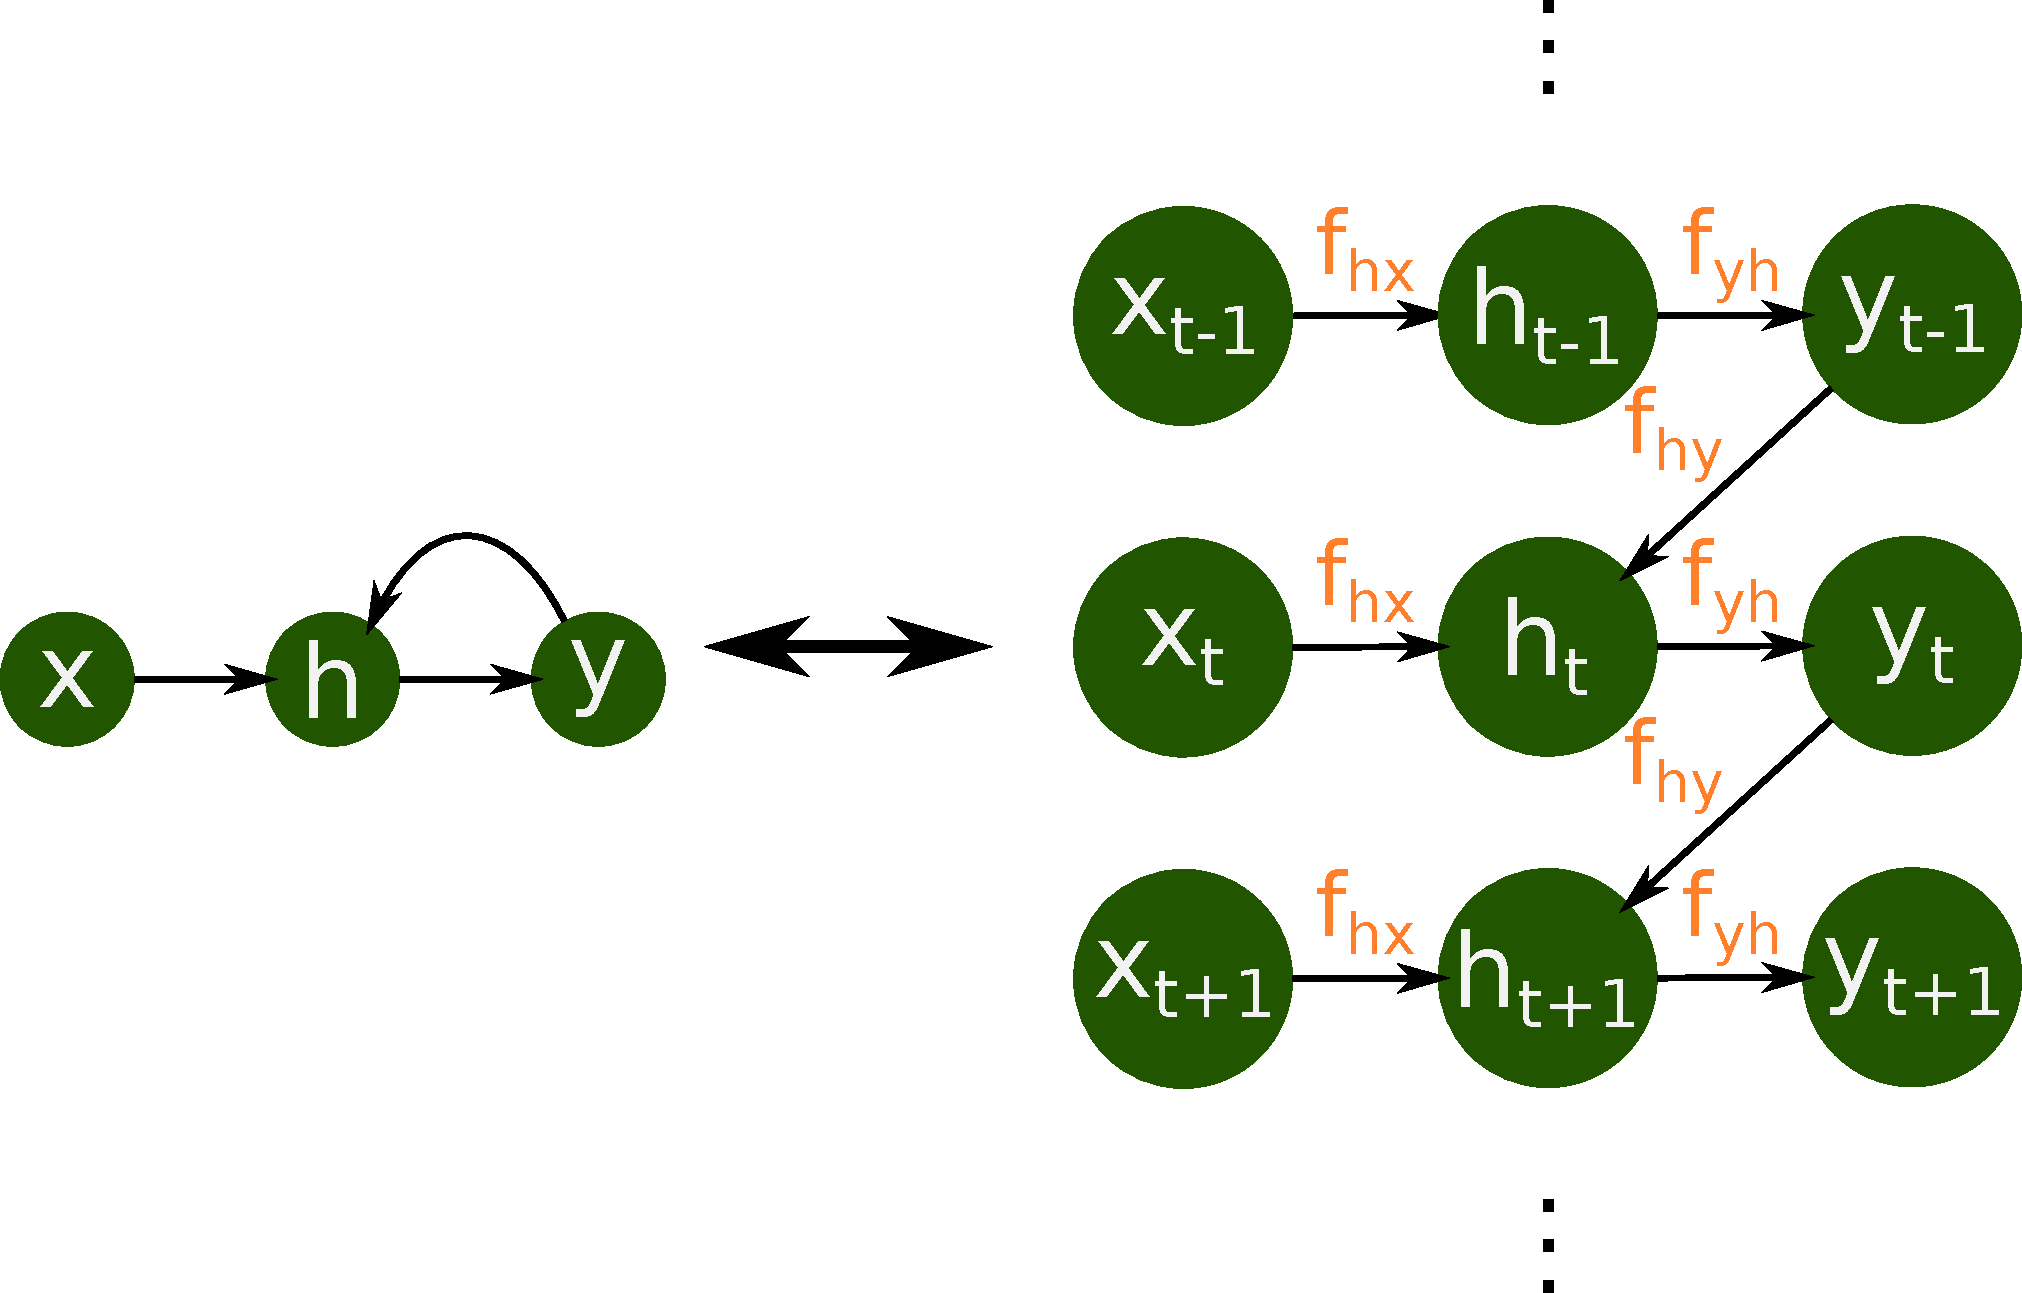
\includegraphics[width=0.7\textwidth]{jordan.pdf}
        \end{center}
        \caption{Redes recorrente de Jordan em suas representações compacta (esquerda) e desenrolada (direita).}
        \label{f:jordan}
      \end{figure}

      \begin{figure}
        \begin{center}
          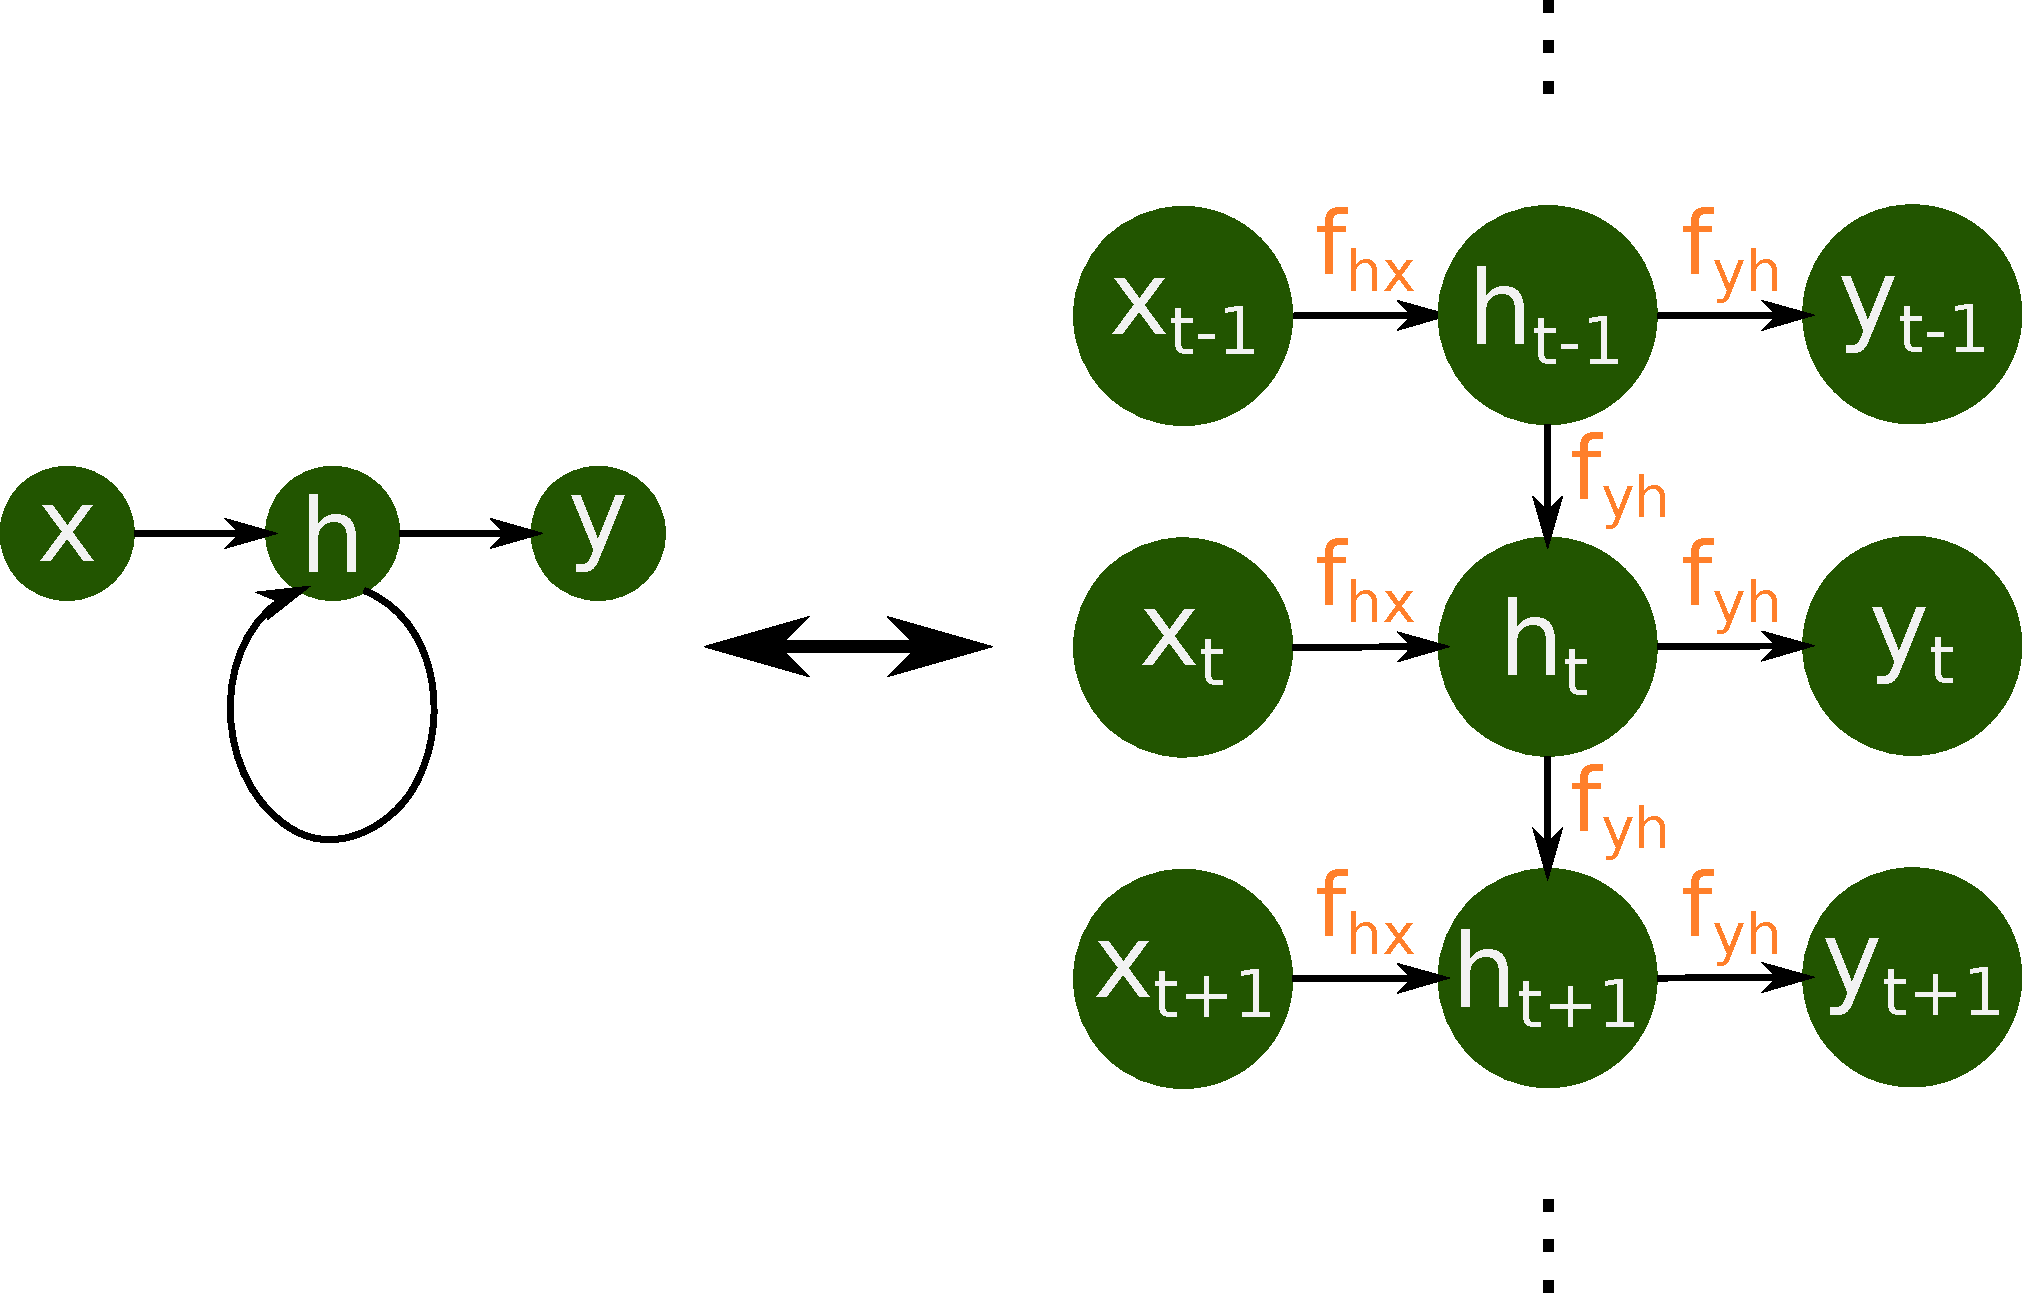
\includegraphics[width=0.7\textwidth]{elman.pdf}
        \end{center}
        \caption{Redes recorrente de Elman em suas representações compacta (esquerda) e desenrolada (direita).}
        \label{f:elman}
      \end{figure}

      As redes neurais recorrentes são por definição redes que permitem grafos com laços de retroalimentação. Por isso, as redes neurais pré-alimentadas são um caso particular das redes retroalimentadas em que nenhum dos nós é retroalimentado na rede. Em detrimento da incrível complexidade que tanto as redes pré-alimentadas como os MLPs, quanto as redes recorrentes, como as de Elman, podem adquirir, estes modelos facilmente se tornam inexplicáveis. O grafo frequentemente apresenta bons resultados em suas aplicações, mas são tão entrelaçados que acaba sendo muito difícil para um ser humano destrinchá-los. Uma vez que os modelos não são compreendidos, o controle que podemos ter sobre eles é pequeno. Muitas alternativas são propostas para aumentar o domínio humano sobre as entranhas das redes neurais. Uma delas é incluir comportamentos conhecidos dentro de suas estruturas. Este é por exemplo o caso das redes neurais informadas de Física (do inglês, \textit{Physics informed neural network} --- PINN). No treinamento de uma PINN insatisfações das respostas geradas a equações físicas são postas na função custo de otimização, de forma que os modelos são treinados para não retornarem resultados intangíveis à realidade. Outra abordagem, a utilizada aqui, é a construção de modelos de redes neurais cujo interior contém equações físicas diretamente. No Capítulo \ref{c:modelagem_por_rnn} é mostrado como construir uma rede de Elman na qual se incorpora um esquema de modelagem física da equação da onda acústica.


\chapter{Modelagem da onda acústica como uma rede neural recorrente} \label{c:modelagem_por_rnn}

  Um simulador da equação da onda é imensa serventia à prospecção de hidrocarbonetos em profundidade, uma vez que esta é fortemente baseada na obtenção de dados sísmicos do alvo. Por meio de um simulador, a inversão destes dados sísmicos em propriedades da subsuperfície se torna possível. Neste capítulo aplicaremos o método das diferenças finitas para resolver a equação da onda acústica bidimensional, e assim fazer simulações numéricas de ondas sísmicas. Mostraremos então como podemos implementar uma rede de Elman, como introduzida em \ref{s:rnn}, que incorpora uma simulação acústica, e cujos parâmetros são as velocidades de propagação acústica do meio propagado. Neste ponto, verifica-se que o procedimento de treinamento de tal rede é equivalente à inversão de forma completa da onda tradicional. Por fim, revisaremos a versão multiescala da inversão de forma completa da onda acústica, a qual será aplicada também ao treinamento da citada rede neural.

  \section{Método das diferenças finitas (FDM)}  \label{s:fdm}

    Considerando a modelagem acústica, isto é, que se pode aproximar o meio modelado a partir de um modelo composto por fluidos, tem-se que a única onda de importância é a onda compressional, a qual pode \DIFaddbegin \DIFadd{ser }\DIFaddend estudada a partir da equação escalar da onda num campo de pressão:

    \begin{equation} \label{e:we}
      \frac{\partial^2 P(t,\vec{r})}{\partial t^2} = v^2\ \nabla^2 P(t,\vec{r})
      ,
    \end{equation}

    \noindent onde $P(t,\vec{r})$ é o campo de pressão, $t$ é o tempo e $\vec{r}$ é uma posição espacial. Com condições iniciais e de contorno dadas, a solução para a equação (\ref{e:we}) é geralmente muito difícil de ser integrada manual ou mesmo simbolicamente. Por isto, aplicações práticas envolvendo sua resolução via de regra utilizam métodos de integração numérica. Um deles é o método das diferenças finitas \DIFdelbegin \DIFdel{, }\DIFdelend \DIFaddbegin \DIFadd{(}\textit{\DIFadd{finite difference method}}\DIFadd{, FDM), }\DIFaddend que consiste em aproximar as derivadas por meio do truncamento de séries polinomiais. Começando pela dimensão do tempo, pode-se calcular o valor do campo $P$ após um pequeno intervalo de tempo $\Delta t$ a partir da série de Taylor:

    \begin{equation} \label{e:serie_p_depois_de_dt}
      P(t+{\Delta t}, \vec{r}) =
        \frac{1}{0!} P(t, \vec{r})
        + \frac{1}{1!} \frac{\partial P(t, \vec{r})}{\partial t}(t) {\Delta t}
        + \frac{1}{2!} \frac{\partial^2 P(t, \vec{r})}{\partial t^2}(t) {\Delta t}^2
        + \frac{1}{3!} \frac{\partial^3 P(t, \vec{r})}{\partial t^3}(t) {\Delta t}^3
        + \cdots
        ,
    \end{equation}

    \noindent por outro lado, pode-se calcular o valor de $P$ antes de um mesmo intervalo $\Delta t$ por:

    \begin{equation} \label{e:serie_p_antes_de_dt}
      P(t-{\Delta t}, \vec{r}) =
        \frac{1}{0!} P(t, \vec{r})
        - \frac{1}{1!} \frac{\partial P(t, \vec{r})}{\partial t}(t) {\Delta t}
        + \frac{1}{2!} \frac{\partial^2 P(t, \vec{r})}{\partial t^2}(t) {\Delta t}^2
        - \frac{1}{3!} \frac{\partial^3 P(t, \vec{r})}{\partial t^3}(t) {\Delta t}^3
        + \cdots
        ,
    \end{equation}

    A soma das séries das equações (\ref{e:serie_p_depois_de_dt}) e (\ref{e:serie_p_antes_de_dt}) pode ser truncado ao termo de segunda ordem, donde obtemos:

    \begin{equation} \label{e:fdm_t}
      \frac{\partial^2 P(t, \vec{r})}{\partial t^2} \approx
      \frac{P(t-{\Delta t}, \vec{r}) - 2P(t, \vec{r}) + P(t+{\Delta t}, \vec{r})}{{\Delta t}^2}
      .
    \end{equation}

    Este resultado implica que um campo de pressão futuro pode ser estimado a partir de suas condições atual e passada:

    \begin{equation} \label{e:fdm_tempo_apenas}
      P(t+\Delta t, \vec{r}) = 2 P(t, \vec{r}) - P(t-\Delta t, \vec{r}) + v^2 {\Delta t}^2 \nabla^2 P(t, \vec{r})
    \end{equation}

    Agora resta calcular o Laplaciano do campo de pressão. No caso bidimensional, esta equação se torna:

    \begin{equation} \label{e:fdm_2d}
      P(t+\Delta t, \vec{r}) = 2 P(t, \vec{r}) - P(t-\Delta t, \vec{r}) + v(\vec{r})^2 {\Delta t}^2 \left(\frac{\partial^2 P(t, \vec{r})}{\partial x^2} +\frac{\partial^2 P(t, \vec{r})}{\partial z^2} \right)
    \end{equation}

    E tal qual foi realizado para o tempo, podemos aproximar uma derivada espacial de $P$ na direção $\vec{r}_s$ por:

    \begin{equation} \label{e:fdm_h}
      \frac{\partial^2 P}{\partial\vec{r}_s^2} (t, \vec{r}) \approx
      \frac{P(t,\vec{r}-{\Delta r}\vec{r}_s) - 2P(t,\vec{r}) + P(t,\vec{r}+{\Delta r}\vec{r}_s)}{{\Delta r}^2}
      ,
    \end{equation}

    \noindent onde $\vec{r}_s$ é uma direção genérica do espaço e $\Delta r$ é uma distância pequena. Assim, considerando uma malha de valores de pressão, o valor de $\frac{\partial^2 P}{\partial\vec{r}_s^2}(t,\vec{r})$ em um ponto $\vec{r}_0$ do espaço pode ser aproximado a partir das pressões no ponto $\vec{r}_0$, no ponto à sua frente e no ponto às suas costas, considerando o sentido de $\vec{r}_s$. Tal tratamento discreto naturalmente resulta no conceito de estêncil de diferenças finitas, ou seja, a geometria de nós de uma malha utilizados em uma operação sobre um de seus pontos. Desta forma, o estêncil de diferenças finitas de segunda ordem para $\frac{\partial^2 P(t,\vec{r})}{\partial r^2}$ na direção $\vec{r}_s$ da malha num ponto $\vec{r}_0$ é $\{\vec{r}_0 - {\Delta r}\ \vec{r}_s, \vec{r}_0, \vec{r}_0+{\Delta r}\ \vec{r}_s\}$ e seus coeficientes são $\{1, -2, 1\}$. O resultado da combinação dos coeficientes com suas pressões associadas pode ser dividido por $\Delta r^2$ para que se obtenha o resultado desejado. Caso a ordem de truncamento da série de Taylor fosse diferente de 2, outro estêncil e coeficientes associados seriam necessários para realizar o cálculo das derivadas. Uma vez que se possui a aproximação adequada de diferenças finitas, pode-se aproximar a equação da onda na equação (\ref{e:fdm_2d}). Por exemplo, utilizando a aproximação de segunda ordem, tanto para o tempo, quanto para o espaço, obtém-se:

    \begin{equation} \label{e:fdm_2d_ordem_2}
      \begin{split}
        P(t+\Delta t,\vec{r}) & =  2 P(t,\vec{r}) - P(t-\Delta t,\vec{r}) \\
          & + v(\vec{r})^2 {\Delta t}^2 \biggm( \frac{P(t, \vec{r}-{\Delta x} \vec{e}_x) - 2P(t, \vec{r}) + P(t, \vec{r}+{\Delta x}\vec{e}_x)}{{\Delta x}^2} \\
          & + \frac{P(t,\vec{r}-{\Delta z} \vec{e}_z)-2P(t,\vec{r})+P(t, \vec{r}+{\Delta z} \vec{e}_z)}{{\Delta z}^2} \biggm)
      \end{split}\DIFaddbegin \DIFadd{,  %DIF >  TODO check if it should be here
    }\DIFaddend \end{equation}

    \DIFaddbegin \noindent \DIFadd{sendo $\vec{e}_x$ e $\vec{e}_z$ os versores na direção dos eixos $x$ e $z$, respectivamente.
}

    \DIFaddend Como a modelagem por diferenças finitas é geralmente realizada utilizando aproximação de segunda ordem no tempo, vale de forma abrangente que se $P$ é dado na forma de uma malha regular de valores discretos, representada matricialmente por $\boldsymbol{P}_{n}$ para o instante $t=t_0+n\Delta t$, onde $t_0$ é o tempo inicial da modelagem, temos que $\boldsymbol{P}_{n+1}$ pode ser calculado por:

    \begin{equation} \label{e:fdm_2d_geral}
      \boldsymbol{P}_{n+1} =
        \boldsymbol{V}^2 {\Delta t}^2
        \nabla^2 \boldsymbol{P}_{n} +
        2 \boldsymbol{P}_{n} -
        \boldsymbol{P}_{n-1}
    \end{equation}

    \noindent onde $\boldsymbol{V}$ é o modelo de velocidades parametrizado como uma matriz que representa valores na mesma malha espacial de $\boldsymbol{P}_t$. A partir da equação (\ref{e:fdm_2d_geral}) pode-se iterativamente prever passos futuros da onda no tempo. Com frequência, porém, deseja-se modelar o comportamento do campo de pressão resultante de alguma excitação sobre o mesmo. Para tal, deve-se adicionar o termo fonte $\boldsymbol{S}_n$ à equação (\ref{e:fdm_2d_geral}) na fase anterior à sua resolução. O termo fonte é função do tempo, e seu valor compõe de $\boldsymbol{P}_{n}$, em que $n=\frac{t-t_0}{\Delta t}$:

    \begin{equation} \label{e:fdm_2d_geral_com_fonte}
      \boldsymbol{P}_{n+1} =
        \boldsymbol{V}^2 {\Delta t}^2
        (\nabla^2 \boldsymbol{P}_{n} + \boldsymbol{S}_{n+1}) +
        2 \boldsymbol{P}_{n} -
        \boldsymbol{P}_{n-1}
        \equiv f(\boldsymbol{V}, \boldsymbol{P}_{n-1}, \boldsymbol{P}_n, \boldsymbol{S}_{n+1})
    \end{equation}

    Nesta equação, $\boldsymbol{S}_{n+1}$ pode ser uma matriz nula em todo ponto diferente do ponto de aplicação do tiro. Matematicamente este caso é equivalente a multiplicar a amplitude $s_n$ da fonte por uma matriz $\boldsymbol{\delta}_{\vec{r}, \vec{r}_s} \equiv \delta_{\vec{r}, \vec{r}_s} \boldsymbol{1}$, na qual $\delta_{\vec{r}, \vec{r}_s}$ é o delta de Kronecker, uma função que zera todas as posições de seu argumento, que não a posição $\vec{r}_s$ da fonte\DIFdelbegin \DIFdel{. }\DIFdelend \DIFaddbegin \DIFadd{, e $\boldsymbol{1}$ é uma matriz com todos os elementos iguais a 1. }\DIFaddend Nesta equação, a função de modelagem recursiva foi chamada de $f$.

    A simulação do pulso que chega num receptor em $\vec{r}_r$ dentro do campo de pressão pode \DIFdelbegin \DIFdel{se }\DIFdelend \DIFaddbegin \DIFadd{ser }\DIFaddend obtida em cada tempo por $\sum_{\vec{r} \in \mathcal{D}} \delta_{\vec{r}, \vec{r}_r} {\boldsymbol{P}_n}$, onde $\mathcal{D}$ é o domínio discreto do modelo, dado pelos índices de $\boldsymbol{P}_n$. Na sísmica, o vetor destas amplitudes para cada tempo é chamado de traço sísmico, e o conjunto de traços sísmicos de cada receptor utilizado é chamado de sismograma.

    Detalhes na implementação do método das diferenças finitas são: a questão da estabilidade numérica, que depende da escolha de um $\Delta t$ que torne a modelagem possível dadas a velocidade máxima do modelo e as distâncias $\Delta x$ e $\Delta z$ utilizadas na malha de discretização; a questão da dispersão, que pode ser causada pela injeção de fontes com frequência muito alta, considerando que um valor limiar é dado em função da velocidade mínima do modelo e dos espaçamentos da malha; e a questão condições de contorno, uma vez que o modelo discretizado possui limites espaciais. Estes pontos são bem sumarizados nas dissertações de mestrado de \shortciteN{santos2013inversao} e \shortciteN{koehne2018fwi}, bem como na tese de doutorado de \shortciteN{andrade2017imageamento}.

    Neste trabalho, os métodos das diferenças finitas, pseudo-espectral e de expansão rápida foram implementados com a condição de contorno atenuadora dada por \shortciteN{cerjan1985nonreflecting}, apesar de só o primeiro deles ser relatado nos resultados. O controle de estabilidade implementado é dado no artigo de \shortciteN{lines1999recipe}, enquanto que o de dispersão considera o critério de \shortciteN{wu1996analysis}.

    A título de curiosidade, vale citar que existem muitos outros métodos para a resolução da equação da onda, entre eles: o método pseudo-espectral \DIFdelbegin %DIFDELCMD < \shortcite{carcione2010generalization}%%%
\DIFdelend \DIFaddbegin \shortcite{kosloff1982forward, carcione2010generalization}\DIFaddend , que envolve calcular o Laplaciano na equação (\ref{e:fdm_2d_geral_com_fonte}) dentro do domínio da frequência, gerando maior exatidão espacial; o método de expansão rápida (\DIFaddbegin \textit{\DIFadd{Rapid expansion method}}\DIFadd{, }\DIFaddend REM), o qual permite marcha no tempo com valores de $\Delta t$ maiores de forma estável, diferentemente do FDM \shortcite{pestana2009rapid}; e o método dos elementos finitos (\DIFaddbegin \textit{\DIFadd{finite element method}}\DIFadd{, }\DIFaddend FEM), que remove a necessidade do uso de uma malha regular \shortcite{carcione2002seismic}. Uma revisão sobre alguns destes métodos está presente em \shortciteN{virieux2011review}.

  \section{Rede de Elman para propagação acústica} \label{s:rnn_modelagem}

    Uma rede recorrente pode ser elaborada para realizar a modelagem por diferenças finitas de segunda ordem no tempo. %citar
    Para tal, monta-se uma rede de Elman de forma que sua célula recorrente, dada pelas equações (\ref{e:elman_ht}) e (\ref{e:elman_yt}), possua:

    \begin{itemize}
      \item $x_t = \boldsymbol{S}_{t}$, onde $\boldsymbol{S}_t$ é o termo fonte no tempo discreto $t$;
      \item $h_t = (\boldsymbol{P}_{t-1}, \boldsymbol{P}_{t})$, onde $\boldsymbol{P}_{t} = f(\boldsymbol{V},h_{t-1}, x_t)$ é o campo de pressão no tempo discreto $t$, sendo $f$ a função de modelagem dada na equação (\ref{e:fdm_2d_geral_com_fonte}) e $\boldsymbol{V}$ o campo discreto de velocidades, parâmetro da rede;
      \item $y_t = \vec{y}_t$, onde $\vec{y}_t$ são as amplitudes de $\boldsymbol{P}_{t}$ nas posições dos receptores.
    \end{itemize}

    \noindent Esta configuração da rede de Elman pode ser vista na Figura \ref{f:elman_modelagem}. Um sismograma é conseguido acumulando os vetores $\vec{y}_t$ como linhas de uma matriz.

      \begin{figure}
        \begin{center}
          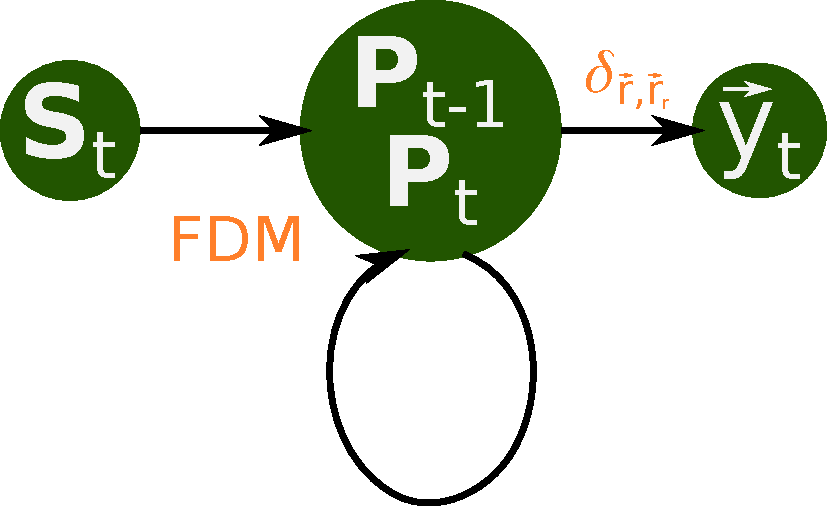
\includegraphics[width=0.3\textwidth]{elman_modelagem.pdf}
        \end{center}
        \caption{Rede recorrente de Elman para modelagem. $\boldsymbol{P}_{t-2}$ e $\boldsymbol{P}_{t-1}$ e $\boldsymbol{S}_t$ são utilizados na composição de um novo par ($\boldsymbol{P}_{t-1}, \boldsymbol{P}_{t})$ por meio de modelagem por diferenças finitas (FDM). $\vec{y}_t$ recebe as amplitudes de $\boldsymbol{P}_{t}$ na posição dos receptores por meio de uma operação $\delta_{\vec{r}, \vec{r}_r}$.}
        \label{f:elman_modelagem}
      \end{figure}

  \section{Inversão de forma completa da onda (FWI)}

    A inversão de forma completa da onda consiste na recuperação dos parâmetros sísmicos em subsuperfície de forma iterativa, a partir da modelagem linearizada de uma equação da onda. Ao contrário de métodos anteriores, em que os tempos de chegada de determinados eventos são invertidos, na FWI constrói-se uma função custo entre as próprias amplitudes do dado adquirido e do dado modelado, a qual deve ser minimizada a partir \DIFdelbegin \DIFdel{aos }\DIFdelend \DIFaddbegin \DIFadd{dos }\DIFaddend parâmetros sísmicos do modelo atual \shortcite{tarantola1984linearized}. Os parâmetros da propagação acústica são tipicamente as velocidades de propagação sísmica no meio estudado, o qual é representado como uma malha de pontos. Caso esta malha seja retangular, podemos aplicar o método das diferenças finitas, como explicado na Seção \ref{s:fdm}, para modelar as amplitudes que chegam nos receptores. Desta forma podemos comparar dados modelados com a função custo escolhida (ver Seção \ref{s:objetivo}) e atualizar o modelo por métodos de inversão linearizada baseados em seu gradiente.

    O desafio do cálculo do gradiente de uma função custo sobre uma modelagem física altamente não-linear é tradicionalmente resolvido a partir do método do estado adjunto \shortcite{fichtner2006adjoint,chen2018neural}. Este método consiste na definição de um problema com variáveis adjuntas, o qual é então utilizado no cálculo do gradiente do problema original com complexidade computacional comparável à resolução do problema direto e independente do número de parâmetros envolvidos \shortcite{johnson2012notes}. Caso o custo de erro quadrático $c(v)=\frac{1}{2}\|\vec{e}\|_2^2=\|\vec{\hat{y}}-\vec{y} \|_2^2$ seja considerado, onde $\vec{\hat{y}}$ é o dado modelado, e $y$ o dado observado, o resultado do método adjunto para a FWI acústica (AFWI) se dá por:

    \begin{equation} \label{e:adjunto}
      \nabla c = \frac{2}{v(t,\vec{r})^3} \int \limits_0^{T} \lambda(t,\vec{r}) \ddot{\hat{P}}(t,\vec{r})\ dt
    \end{equation}

    \noindent onde $v$ é o campo de velocidade do modelo e $\hat{P}$ é o campo de pressão modelado e $\lambda$ é o campo adjunto que satisfaz à equação \shortcite{santos2013inversao}:

    \begin{equation} \label{e:adjunta}
      \frac{1}{v(\vec{r})^2} \frac{\partial^2 \lambda(t,\vec{r})}{\partial t^2} =
      \nabla^2 \lambda(t,\vec{r}) + (\hat{y} - y)
    \end{equation}

    \noindent onde $\hat{y}$ é o dado calculado e $y$ é o dado observado. Há muita semelhança entre esta equação e a equação da onda acústica. De fato, a solução de $\lambda$ na equação \ref{e:adjunta} é obtida pela propagação reversa do resíduo do dado modelado de forma reversa no tempo, por conta das condições de contorno a seguir:

    \begin{equation} \label{e:adjunta_condicoes}
      \begin{cases}
        \lambda(t=T,\vec{r}) = 0\\
        \frac{\partial \lambda}{\partial t}(t=T,\vec{r}) = 0\\
      \end{cases}
    \end{equation}

    Assim, o método adjunto envolve uma modelagem que parte de condições iniciais para calcular $\hat{P}$ e outra, de condições finais, para a obtenção de $\lambda$. O somatório do produto destes campos na equação \ref{e:adjunto} pode ser enxergado como uma migração dos resíduos utilizando uma condição de imagem de correlação cruzada \DIFdelbegin \DIFdel{\mbox{%DIFAUXCMD
\cite{virieux2009overview,biondi1999wave}}\hspace{0pt}%DIFAUXCMD
}\DIFdelend \DIFaddbegin \shortcite{virieux2009overview,biondi1999wave}\DIFaddend .


  \section{Inversão como treinamento de uma rede recorrente de Elman}

    O método adjunto é extremamente eficiente no cálculo do gradiente da função custo na FWI, entretanto, sua utilização em um problema de inversão sobre outro fenômeno físico exigiria uma nova formulação para a variável adjunta, à qual a implementação do gradiente se tornaria secundária. A escrita processos de simulação física como redes neurais, ou mais precisamente, como grafos num esquema de diferenciação automática, tem como vantagem que o cálculo do gradiente pode ser realizado imediatamente após a implementação do operador de simulação. Aliado a isto, prova-se (ver Apêndice \ref{a:equivalencia_fwi_rnn}) que a diferenciação automática calcula o gradiente da função custo de erro quadrático de forma equivalente ao procedimento realizado no método adjunto.

    Outro ponto positivo do tratamento de processos de modelagem como redes neurais é a inclusão do problema no contexto do aprendizado de máquina. Atualmente existem diversos ambientes com todo o ferramental necessário para treinar modelos de aprendizado de máquina com eficiência e controle. Entre eles o TensorFlow \shortcite{abadi2015tensorflow}, o JAX \shortcite{jax2018github}. Tais ambientes provêem ao usuário formas rápidas e reutilizáveis de realizar operações em diferentes tipos de unidades de processamento, de implementar otimizadores estocásticos, de desenvolver novos tipos de interrupção precoce e muito mais.

    Ainda assim, o método adjunto está longe de ser descartado. O conhecimento da solução analítica que o método adjunto proporciona por natureza pode abrir novas janelas para otimização. No caso da FWI, por exemplo, a implementação do método adjunto se inicializa pela multiplicação do campo primário no tempo inicial $P(t_0)$ pelo campo adjunto $\lambda$ no mesmo instante. O campo adjunto inicial, por sua vez, depende das condições finais da modelagem, as quais são por sua vez dependentes do último campo primário modelado. Isto implica que na solução do método adjunto, e por consequência naquela realizada na diferenciação automática, por padrão é necessário guardar todos os campos primários da modelagem na memória para então proceder com a resolução do campo adjunto e do gradiente da função custo. Desta forma, seu cálculo depende de grandes volumes de memória. Ter acesso à equação do gradiente do método adjunto nos permite utilizar técnicas para minimizar o uso de memória, de forma a salvar apenas o mínimo de passos temporais da modelagem primária para estimar a intergral da equação (\ref{e:adjunto}).


  \section{Inversão multiescala}

    Um tópico importante sobre a inversão sísmica é que os dados modelados possuem uma frequência bastante elevada, o que faz com que durante a inversão os picos de um determinado evento sísmico modelado possam estar mais próximos de um outro evento sísmico no dado observado ao invés de seus verdadeiros pares. Assim, no cálculo da função custo, a comparação será feita entre eventos que não são verdadeiramente correlacionados resultando num mínimo local que pode prejudicar a busca por um modelo mais verdadeiro. Este fenômeno é conhecido pelo termo \emph{salto de ciclo} \DIFdelbegin %DIFDELCMD < \shortcite{santos2013inversao,koehne2018fwi}%%%
\DIFdelend \DIFaddbegin \shortcite{virieux2009overview}\DIFaddend , e pode ser evitado por meio de uma abordagem multiescala da FWI \DIFaddbegin \shortcite{bunks1995multiscale}\DIFaddend .

    A FWI multiescala desempenha modelagens em frequências crescentes --- e portanto com escalas espaciais decrescentes --- as quais são comparadas com os dados filtrados com passa-baixa de frequência máxima equivalente. Desta forma evita-se que a inversão comece a otimizar determinado evento antes de localizar sua origem no campo de velocidades corretamente. Para cada banda de frequência, uma série de iterações do método gradiente escolhido são realizadas considerando dados filtrados. A fonte utilizada na modelagen, por sua vez, deve sempre possuir conteúdo de frequência compatível com os dados em uso.

    O esquema multiescala também é aplicável à FWI formulada como treinamento de uma rede recorrente. Para tal, treina-se os parâmetros da rede uma vez para cada escala mantendo sempre os parâmetros treinados sob a banda de frequência anterior como parâmetros iniciais da próxima.

\chapter{Metodologia e Resultados}

  \section{Metodologia}

    A metodologia deste trabalho envolve a implementação de uma rede recorrente de Elman que incorpora a equação da onda acústica em sua formulação por meio da técnica das diferenças finitas e é capaz de realizar modelagem. Para isto o modelo descrito na seção \ref{s:rnn_modelagem} foi implementado na linguagem Python. Num primeiro momento, foi utilizada a biblioteca de diferenciação automática e aceleração em diferentes unidades de processamento \emph{JAX} \shortcite{jax2018github}, entretanto após a implementação da modelagem direta foi percebido um \textit{bug} da biblioteca na autodiferenciação reversa da operação de convolução, a qual é utilizada no cálculo do Laplaciano durante a propagação da onda\footnote{Ver discussão em \url{https://github.com/google/jax/discussions/8411}.}, o que zerava as saídas do gradiente fora da região dos receptores. Uma nova implementação foi então realizada utilizando as ferramentas da biblioteca \emph{TensorFlow} \shortcite{abadi2015tensorflow}, a qual obteve êxito na autodiferenciação reversa.

    Tal rede implementada possui como parâmetro um modelo de velocidades de propagação da onda acústica em forma matricial. Em posse da rede modeladora, escolheu-se o modelo Marmousi (Figura \ref{f:modelo_real_borrado}) com 187 amostras de profundidade e 184 na horizontal para gerar os dados sintéticos. O modelo utilizado possui escala duas vezes menor que a original \shortcite{brougois1990marmousi}, pois as operações de modelagem e diferenciação reversa exigem mais poder computacional e memória do que as disponíveis durante a realização de testes em tempo hábil para a escrita deste material. Para a realização da modelagem de 31 sismogramas cujos tiros foram equiespaçados pela superfície do modelo. Os espaçamentos vertical e horizonal entre nós foram respectivamente iguais a 16 e 50 m. A assinatura da fonte escolhida para os tiros foi uma onda Ricker de frequência igual a 8 Hz, a maior frequência modelável para os espaçamentos da malha de diferenças finitas pelo critério dado em \shortciteN{wu1996analysis}, enquanto que o intervalo $\Delta t$ de amostragem dos receptores foi de $4$ ms, com número de amostras suficientes para a modelagem de 4 s de dados. Foi considerada a geometria de aquisição sísmica \textit{split-spread} com afastamento mínimo igual a 500 m, afastamento máximo dado pelos limites do modelo, e afastamento entre receptores igual a 50 m.

    A onda direta não é útil à inversão em profundidade, uma vez que a mesma não interage com os volumes mais profundos do modelo. Infelizmente este evento carrega o maior conteúdo de energia do dado sísmico. Inverter um dado com esta característica pode levar o modelo a mínimos locais da função custo, como já relatado por \shortciteN{koehne2018fwi}. Isto também foi experienciado durante a elaboração dos experimentos deste trabalho. Uma solução comum para este problema é a retirada da onda direta dos sismograma gerado por meio do silenciamento de suas amplitudes. Em dados reais, isto pode exigir uma etapa manual de seleção destes eventos, mas como dados sintéticos foram aqui utilizados, a forma mais simples de produzir tal silenciamento é subtraindo dos sismogramas modelados, outros sismogramas, estes simulados a partir de uma versão diferente do modelo, a qual possui apenas informações superficiais --- e que portanto só gerará as ondas diretas. Após esta etapa, restam no dado os eventos mais importantes à FWI. Alguns sismogramas das modelagens sem onda direta realizados podem ser vistos na Figura \ref{f:sismogramas_sinteticos}, enquanto que um exemplo de silenciamento de dados sintéticos como o relatado há pouco é mostrado na Figura \ref{f:remocao_onda_direta} para um modelo de duas interfaces.

    Os dados calculados com o modelo real foram então passados à categoria de dados reais observados em campo, para que se pudesse testar a capacidade de inversão por treinamento da rede recorrente. Nesta nova etapa, considerou-se um modelo inicial dado por um filtro de média móvel com tamanho de janela igual a $30\times30$ sobre o modelo verdadeiro, cujo resultado é uma versão de baixa resolução do modelo real e pode ser aludido a um modelo obtido por uma prévia análise de velocidades do processamento sísmico tradicional. O modelo Marmousi real e o borrado podem ser vistos na Figura \ref{f:modelo_real_borrado}. Mesmo tomando as precauções com a onda direta descrita há pouco, valores muito intensos foram encontrados na parte superficial dos gradientes calculados, os quais instabilizavam a otimização do modelo. Por isso, os gradientes calculados nas primeiras 8 amostras do modelo foram zerados ao longo da inversão. Esta região não foi alterada durante a geração do modelo inicial.

      \begin{figure}
        \begin{center}
          \includegraphics[width=0.9\textwidth]{modelo_real_borrado.pdf}
        \end{center}
        \caption{Modelo Marmousi real utilizado na produção dos dados sintéticos (A) e modelo borrado utilizado como ponto inicial da para o treinamento da rede (B).}
        \label{f:modelo_real_borrado}
      \end{figure}

      \begin{figure}
        \begin{center}
          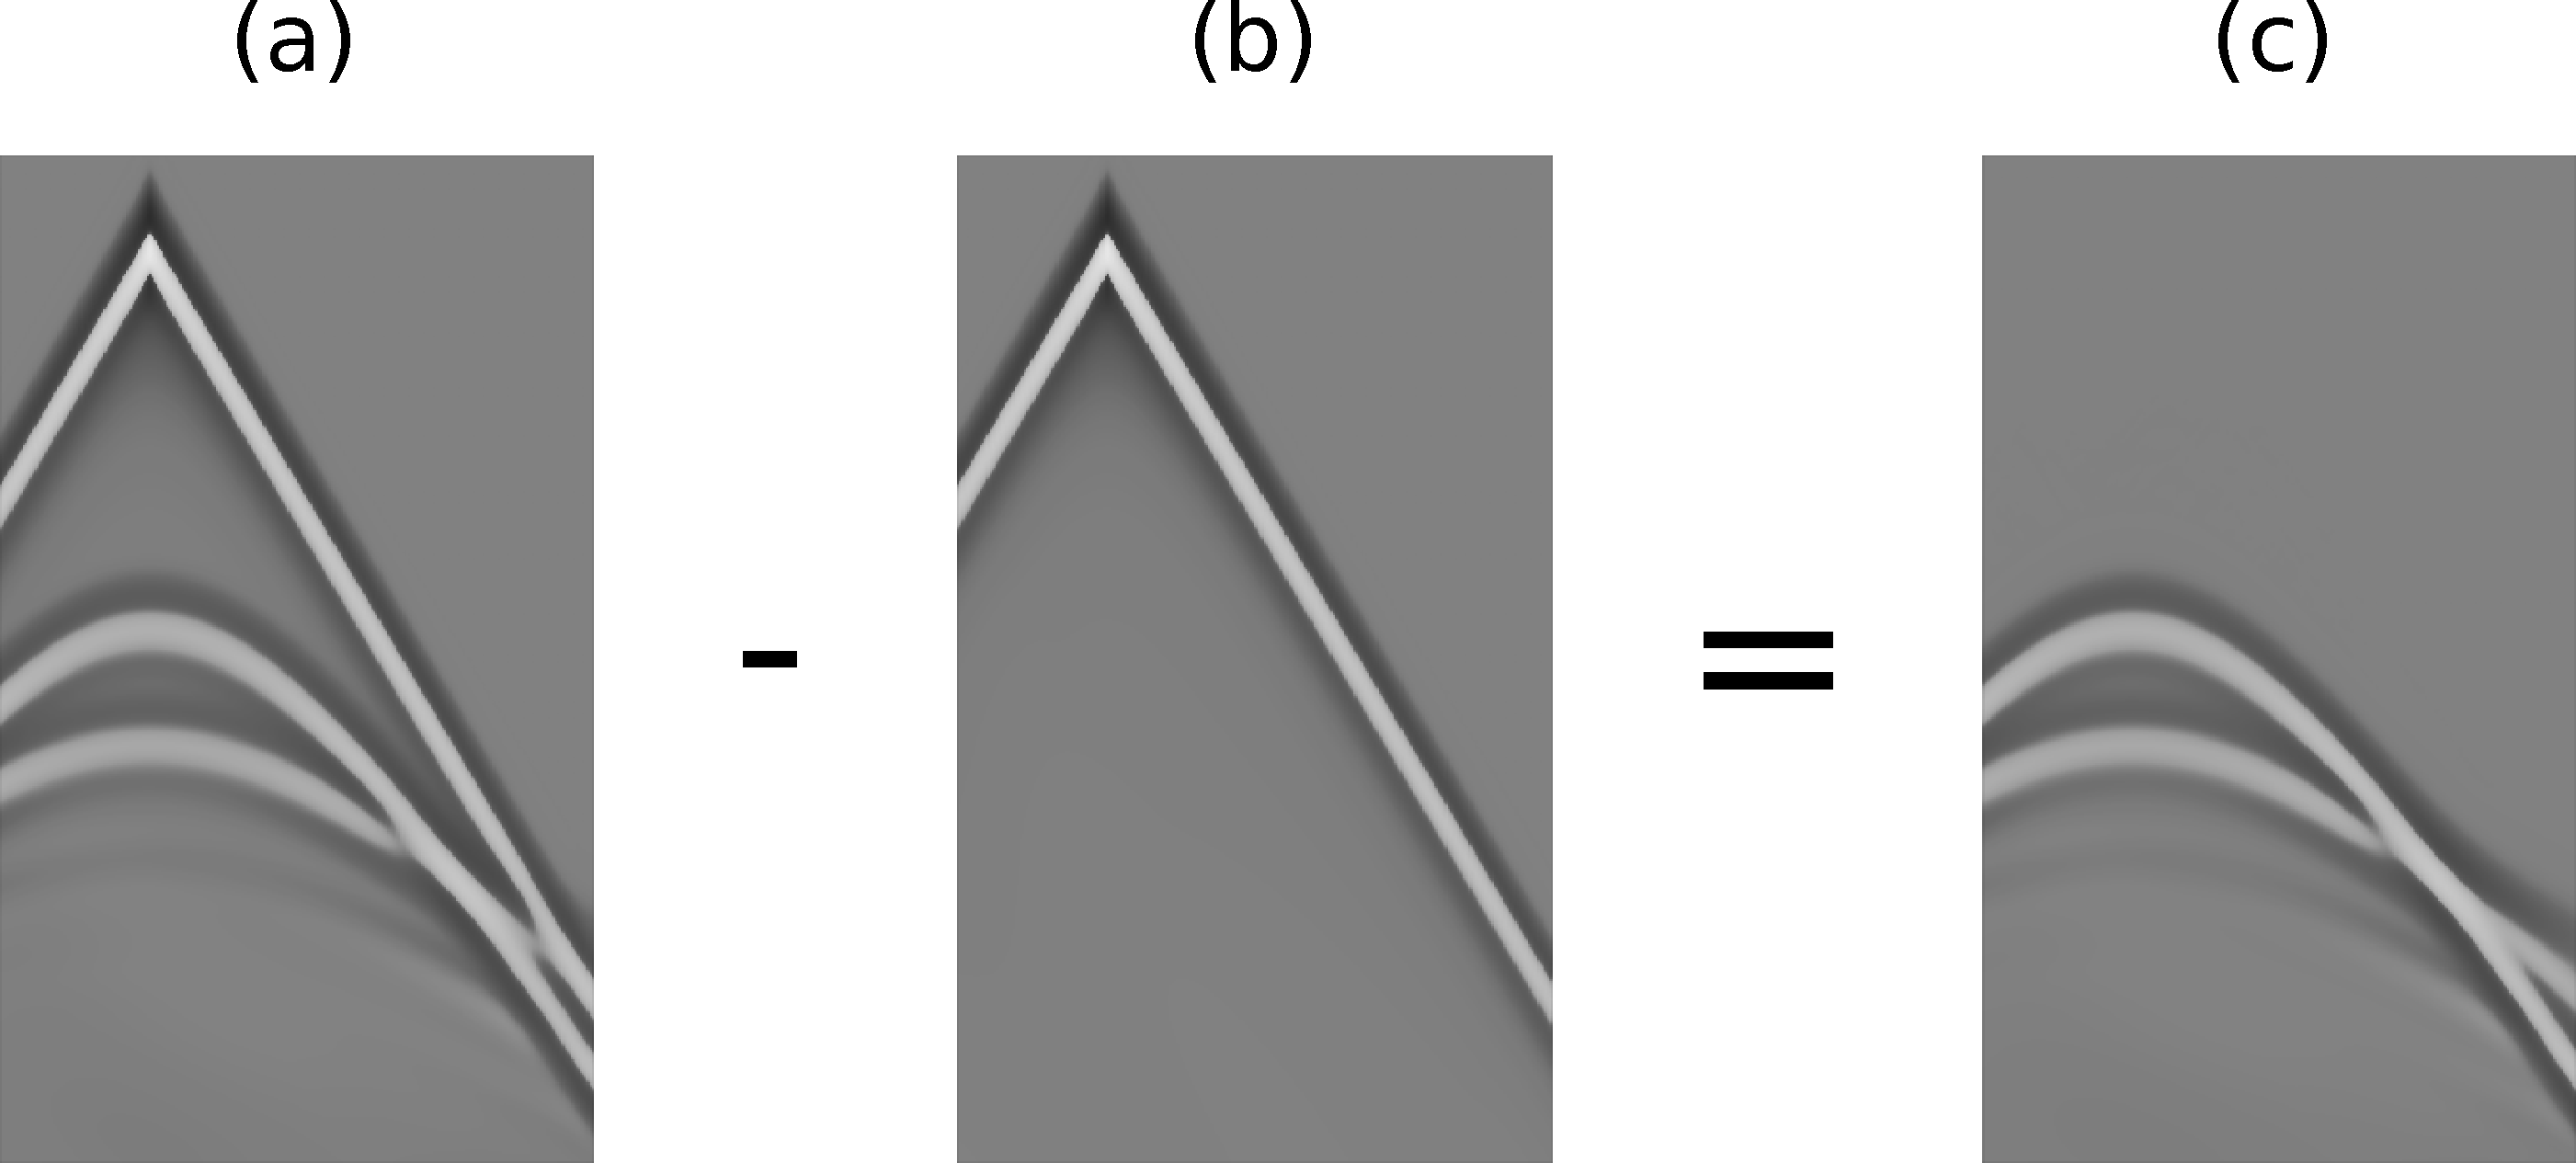
\includegraphics[width=0.5\textwidth]{remocao_onda_direta.pdf}
        \end{center}
        \caption{Modelagem de sismograma num modelo de duas interfaces em (a), modelagem de onda direta do mesmo tiro em (b) e subtração de (a) por (b) em (c), na qual se apresentam apenas os eventos de reflexão e refração.}
        \label{f:remocao_onda_direta}
      \end{figure}


      \begin{figure}
        \begin{center}
          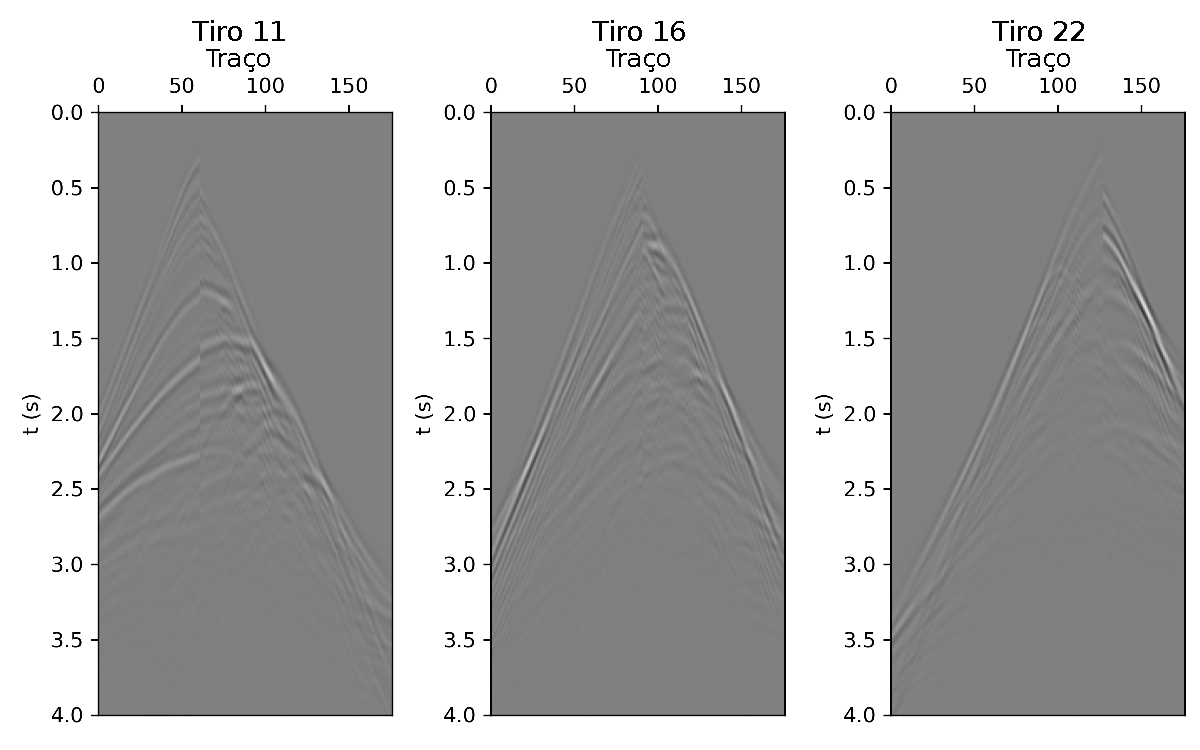
\includegraphics[width=0.9\textwidth]{sismogramas_sinteticos.pdf}
        \end{center}
        \caption{Da esquerda para a direita se apresentam os sismogramas: do décimo primeiro tiro, do décimo sexto tiro, e do vigésimo segundo tiro.}
        \label{f:sismogramas_sinteticos}
      \end{figure}

    Para a fase de inversão foram testados os algoritmos SGD, Momento e Adam para a atualização dos parâmetros, utilizando um tiro por lote. Para eles, o MSE foi utilizado como função custo, e seu gradiente foi calculado por diferenciação automática reversa. Além disto, três quartos dos dados (24 tiros) foram utilizados para o treinamento da rede, enquanto que o restante deles foi aleatoriamente escolhido para validação dos resultados. A partir desta separação, utilizou-se uma estratégia de interrupção precoce como a descrita na Seção \ref{s:interrupcao_precoce} para controle, de forma a evitar o sobreajuste do modelo. Nela o critério de paciência utilizado foi de 6 épocas, de forma que, caso não seja vista melhora na função custo sobre os tiros de validação após tal período\DIFaddbegin \DIFadd{, }\DIFaddend a otimização \DIFdelbegin \DIFdel{foi }\DIFdelend \DIFaddbegin \DIFadd{é }\DIFaddend cessada. A modelagem direta utilizada na inversão já incorpora o silenciamento da onda direta da mesma maneira utilizada na geração dos dados sintéticos.

    A abordagem multiescala de inversão foi adotada. Para tal, foram consideradas três bandas de frequência compreendidas de 0 até respectivamente: 2.7, 5.3 e 8 Hz. O sismograma do tiro 11 pode ser visto em suas três bandas de frequências na Figura \ref{f:sismogramas_frequencias}. Para cada banda de frequência a estratégia de interrupção precoce foi reinicializada e os parâmetros inicializados a partir do melhor modelo obtido durante a banda de frequência anterior, e apenas um valor máximo de 30 épocas de otimização eram permitidas.

    \begin{figure}
      \begin{center}
        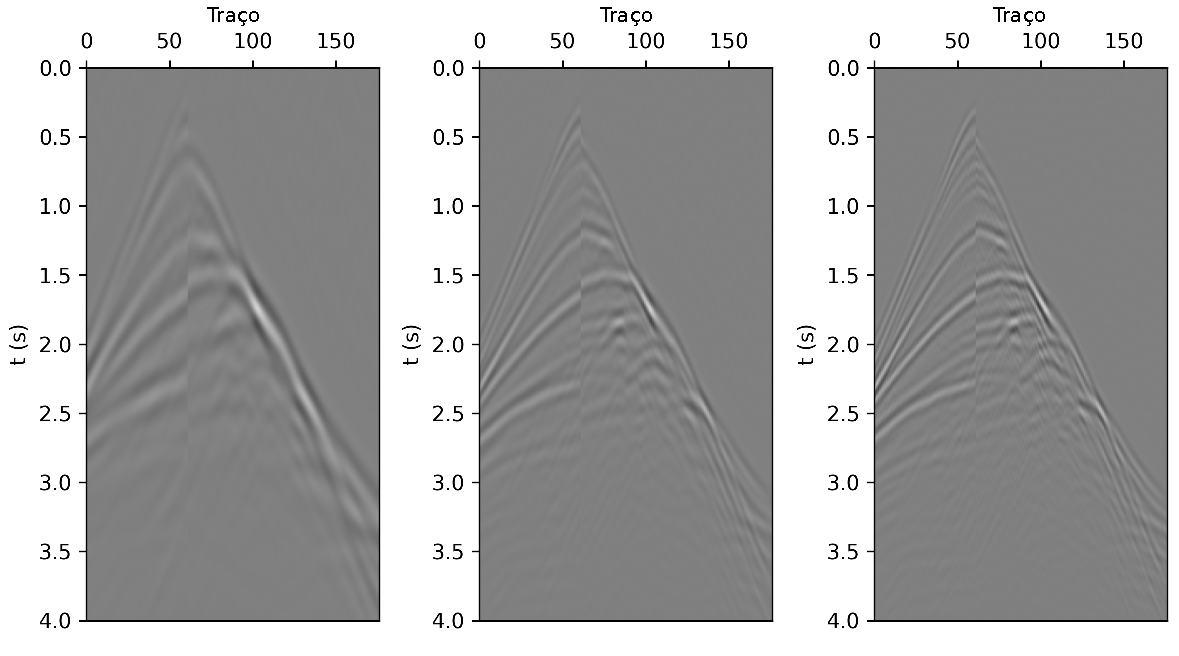
\includegraphics[width=0.9\textwidth]{sismogramas_frequencias.pdf}
      \end{center}
      \caption{Mesmo sismograma modelado com fontes de frequência: 2,7 $Hz$, 5.3 $Hz$, e 8 $Hz$, da esquerda para a direita. Observe como algumas feições do sismograma das frequências mais altas não são visíveis em baixas frequências.}
      \label{f:sismogramas_frequencias}
    \end{figure}


  \section{Resultados da inversão}

    Um fator muito importante a ser selecionado durante a inversão por métodos baseados em gradiente é o seu passo ou taxa de aprendizado, $\eta$, o qual varia a depender do problema e do método de otimização. Nos métodos com mais parâmetros, como o Momento e o Adam, o melhor passo varia também com seus outros parâmetros de otimização. Uma taxa de aprendizado nula não atualiza o modelo, uma pequena pode levar a mínimos locais da função custo, enquanto que valores muito grandes podem fazer os parâmetros divergirem. Neste trabalho, bons valores para $\eta$ foram obtidos por tentativa e erro em cada caso. Os outros parâmetros de otimização, tanto do algoritmo Momento ($\alpha$), quanto do Adam ($\beta_1$ e $\beta_2$), foram mantidos com seus valores tradicionais, uma vez que a otimização não melhorou com suas modificações. Assim, os seguintes parâmetros foram utilizados nos métodos testados:

    \begin{itemize}
      \item SGD: $\eta=10^6$;
      \item Momento: $\eta=10^6$, $\alpha=0,9$; e
      \item Adam: $\eta=10$, $\beta_1=0,9$, $\beta_2=0,999$.
    \end{itemize}

    \begin{figure}
      \begin{center}
        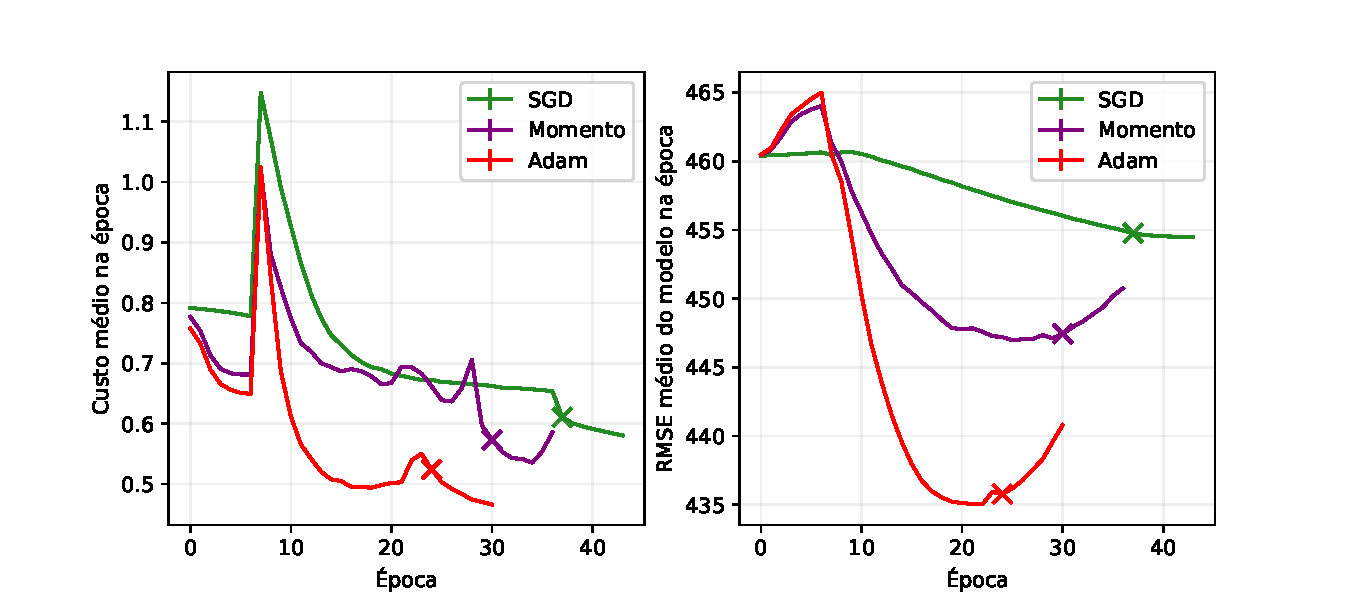
\includegraphics[width=0.9\textwidth]{curvas_custo.pdf}
      \end{center}
      \caption{Função custo (esquerda) e erro médio (direita) do modelo em função das épocas de otimização \DIFdelbeginFL \DIFdelFL{apra }\DIFdelendFL \DIFaddbeginFL \DIFaddFL{para }\DIFaddendFL cada modelo.}
      \label{f:curvas_custo}
    \end{figure}

    As curvas de aprendizado utilizando cada método podem ser vistas em função das épocas de iteração na Figura \ref{f:curvas_custo}. Um ponto importante no gráfico do custo médio por época são os saltos de comportamento nas curvas, os quais valem uma importante discussão. Estes pontos coincidem com o aumento da frequência de modelagem, e, portanto, com o aumento da frequência dos dados envolvidos na função custo, algo que os algoritmos de otimização de uso comum não levam em consideração em sua teoria. Felizmente, existem abordagens automatizadas hoje para lidar com este problema: os autores \shortciteN{bernal2021accelerating} propõem uma forma de lidar com este problema por meio da variação da taxa de aprendizado em função da época de otimização e, principalmente, das bandas de frequência utilizadas na FWI. Esta faz parte de uma classe de soluções chamada de agendamento (do inglês, \textit{scheduling}), entretanto este tema não foi tratado no presente material.

    Outro ponto importante na Figura \ref{f:curvas_custo} é o papel fundamental da interrupção precoce no controle da FWI. Nas curvas da função custo média, podemos perceber duas discontinuidades, as quais estão ligadas à variação de escala da FWI. Podemos apontar no gráfico, que para cada nova frequência, a função custo decai com as épocas até determinado valor, mas mesmo quando ainda decaindo, a otimização é parada, o que especialmente visível durante o primeira e última bandas de frequência utilizadas. O critério de parada da otimização explica: para cada parada, a função custo sobre os tiros de controle não decai ou até mesmo aumenta pelas últimas 6 iterações. A função custo representa de forma preliminar o desejo de obter um modelo cujas saídas sejam similares às da realidade, mas nosso verdadeira vontade é minimizar o erro entre o modelo que possuímos e o modelo real. \DIFdelbegin \DIFdel{A modelagem é apenas uma abstração para este objetivo. A vantagem de }\DIFdelend \DIFaddbegin \DIFadd{Deste modo, uma vantagem em }\DIFaddend utilizarmos dados sintéticos para testar algoritmos de inversão é que sabemos a resposta e podemos calcular o erro do modelo diretamente. Com base nisto, vemos no segundo gráfico da mesma figura, que para cada vez que uma frequência foi interrompida, o erro entre modelos estava aumentando --- mesmo que a função custo de treinamento estivesse decaindo. Tiros de controle e a utilização da interrupção precoce evitam o sobreajuste na FWI, assim como nos métodos de aprendizado de máquina supervisionados.

    Nas Figuras \ref{f:inversoes_freq_1} e \ref{f:inversoes_freq_2} podemos ver, respectivamente, o resultado da última iteração dos métodos de otimização testados nas duas primeiras bandas de frequências da FWI multiescala realizada por meio do treinamento da rede recorrente, enquanto que na Figura \ref{f:inversoes_freq_3}, podemos ver o melhor modelo obtido na última banda de frequência da inversão. Na Figura \ref{f:variacoes_desde_inicio} são mostradas as diferenças entre o modelo final obtido e o modelo inicial. De forma geral, o SGD consegue recuperar razoavelmente as velocidades mais próximas à superfície, convergindo em 43 épocas. O método do Momento atravessa espaço de modelos com inércia das otimizações passadas e consegue inverter melhor nas profundidades médias a altas após 34 épocas. O método Adam supera os resultados dos outros dois métodos com o menor número de épocas necessárias para convergência. Em 30 épocas, o método consegue o menor valor da função custo e menor diferença com relação aos parâmetros reais. No método Momento e no Adam, é possível imagear \DIFdelbegin \DIFdel{em }\DIFdelend sensivelmente as camadas mais profundas do modelo, aos 2,700 metros sob a superfície.

    A análise do perfil vertical de velocidades em $x=2500$ m mostrado na Figura \ref{f:perfil_velocidades} demonstra que as informações de mais alta frequência foram melhor identificadas utilizando os métodos Momento e Adam, sendo que o último obteve as amplitudes de velocidade mais próximas do modelo verdadeiro.

    \begin{figure}
      \begin{center}
        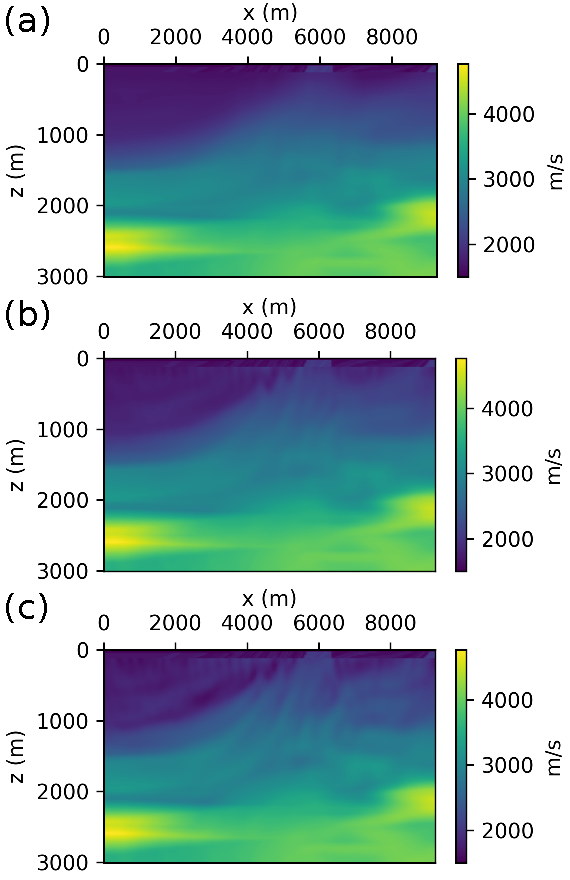
\includegraphics[width=0.6\textwidth]{inversoes_freq_1.pdf}
      \end{center}
      \caption{Modelo obtido na última época de otimização durante a etapa de modelagem sob a banda de frequência de 0 a 2.7 $Hz$ usando SGD (a), Momento (b) e Adam (c).}
      \label{f:inversoes_freq_1}
    \end{figure}

    \begin{figure}
      \begin{center}
        \includegraphics[width=0.6\textwidth]{inversoes_freq_2.pdf}
      \end{center}
      \caption{Modelo obtido na última época de otimização durante a etapa de modelagem sob a banda de frequência de 0 a 5.3 $Hz$ usando SGD (a), Momento (b) e Adam (c).}
      \label{f:inversoes_freq_2}
    \end{figure}

    \begin{figure}
      \begin{center}
        \includegraphics[width=0.6\textwidth]{inversoes_freq_3.pdf}
      \end{center}
      \caption{Melhor modelo obtido durante a otimização na última banda de frequência (0 a 8 $Hz$) usando SGD (a), Momento (b) e Adam (c).}
      \label{f:inversoes_freq_3}
    \end{figure}

    \begin{figure}
      \begin{center}
        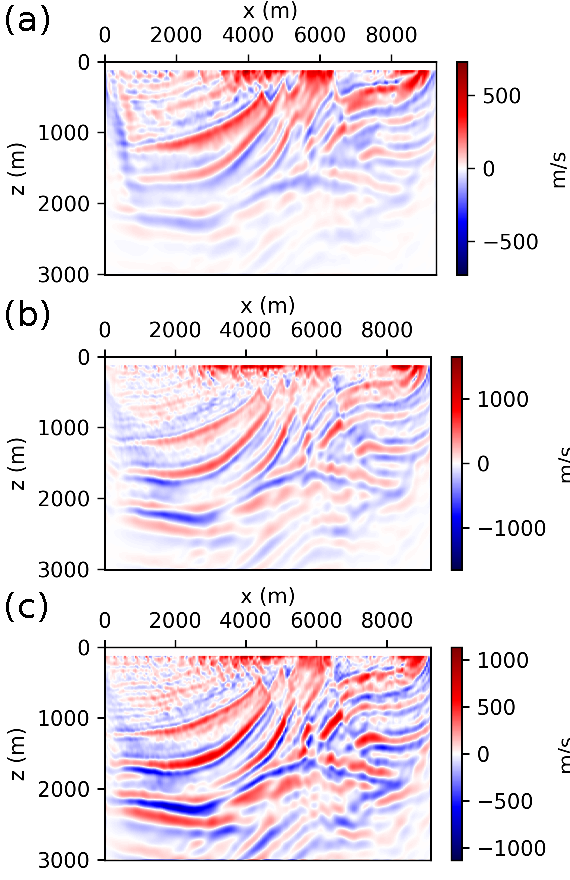
\includegraphics[width=0.6\textwidth]{variacoes_desde_inicio.pdf}
      \end{center}
      \caption{Diferença entre o melhor modelo obtido na FWI multiescala e o modelo inicial para os métodos: SGD (a), Momento (b) e Adam (c).}
      \label{f:variacoes_desde_inicio}
    \end{figure}

    \begin{figure}
      \begin{center}
        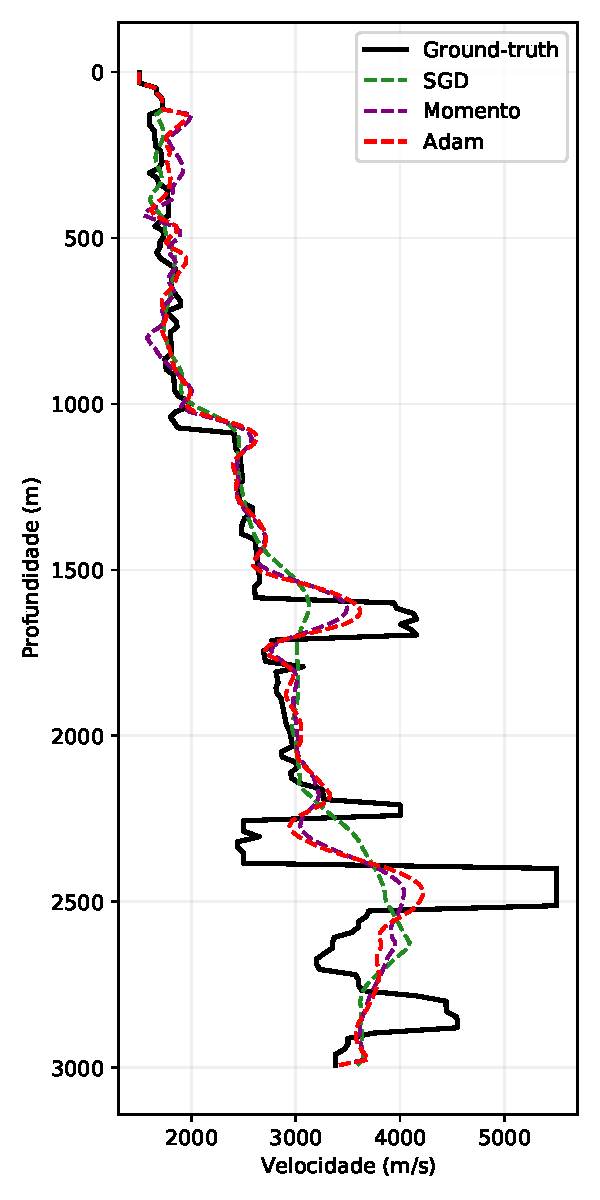
\includegraphics[width=0.5\textwidth]{perfil_velocidades.pdf}
      \end{center}
      \caption{Perfil vertical de velocidades em $x=2.500$ m para o modelo verdadeiro (preto) e os modelos resultantes da FWI por meio do método SGD (tracejada em verde), Momento (tracejada em lilás) e Adam (tracejada em vermelho).}
      \label{f:perfil_velocidades}
    \end{figure}

    Em todas as inversões, mas em especial no caso dos otimizadores Adam e Momento, são visíveis artefatos de maior velocidade e até mesmo a presença de bandamentos com orientação contrária à direção de acamamento das estruturas geológicas reais. Este problema pode ser devido à baixa quantidade de tiros utilizada na inversão, mas uma investigação mais aprofundada deve ser feita para uma maior compreensão do problema.

%%%%%%%%%%%%%%%%%%%%%%%%%%%%%%%%%%%%%%%%%%%%%%%%%%%%%%%%%%%%%%%%%%%
%                                                                 %
%                         CONCLUSOES                              %
%                                                                 %
%%%%%%%%%%%%%%%%%%%%%%%%%%%%%%%%%%%%%%%%%%%%%%%%%%%%%%%%%%%%%%%%%%%

\chapter{Conclusões}

  Neste material foram introduzidos os conceitos básicos de aprendizado estatístico, seus métodos de otimização e a extensão de seus modelos mais simples às redes neurais. A extensão da rede neural recorrente de Elman para um modelo capaz de realizar simulações acústicas foi teorizada e implementada, gerando resultados satisfatórios de modelagem e inversão utilizando três otimizadores típicos do universo das redes neurais: SGD, Momento e Adam. Problemas de otimização multi-frequência devem ser corrigidos em trabalhos futuros por meio da implementação de técnicas de agendamento no processo de otimização, as quais são tidas como tecnologias relativamente avançadas de treinamento de redes. Uma pequena inadequação próxima à superfície dos modelos invertidos foi encontrada, a qual é uma suposta consequência do uso de poucos tiros para a inversão, mas que deve ser alvo de futuras investigações. É necessário salientar que, apesar da possibilidade de realização da FWI pelo método aqui apresentado, a demanda por memória no cálculo dos gradientes se torna superior à comumente utilizada em casos de aplicação real. Em casos similares, a solução do método adjunto pode permitir a implementação de otimizações valorosas.

  Do ponto de vista da modelagem tradicional, a generalidade do método empregado abre janelas à pesquisa neste e em outros problemas físicos, como a dispersão de poluentes em fluidos, a dissipação de calor ou a modelagem de deformações numa estrutura mecânica, uma vez que a inversão aqui realizada acontece por diferenciação automática, sem mesmo o uso explícito do método adjunto. Este ponto é muito valoroso, pois o método adjunto exige uma etapa de pré-formulação de sua teoria com relação ao problema estudado da qual sua implementação depende, enquanto que a inversão por diferenciação automática é de implementação imediata para qualquer problema que pode ser expresso num grafo de computações comuns com diferenciais conhecidas. Uma contribuição interessante vinda do contexto das redes neurais é a de interrupção precoce, técnica que permitiu uma inversão controlada na FWI aqui implementada. Desta forma, ao invés de um número fixo de iterações de otimização, um critério de parada baseado na modelagem sobre tiros de validação do campo de velocidades otimizado foi implementado.

  Do ponto de vista das redes neurais, este trabalho \DIFdelbegin \DIFdel{constroi }\DIFdelend \DIFaddbegin \DIFadd{constrói }\DIFaddend uma rede com bons resultados e parâmetros facilmente interpretáveis --- as velocidades em subsuperfície. A junção da área das redes com a da inversão acústica traz uma ideia não muito comum ao treinamento das redes: é possível que um treinamento multiescala seja útil para também para o treinamento de outras redes neurais. Esta ideia é diretamente aplicável a redes de segmentação semântica, por exemplo. Vale citarmos que a metodologia das redes neurais informadas de física --- isto é, a penalização de insatisfações de equações físicas dentro da função custo utilizada na inversão --- é um próximo passo a ser introduzido ao modelo físico desenvolvido neste material e tratado em trabalhos futuros.

  Creio que este material é adequado à leitura por estudantes da Geofísica que desejem ser introduzidos ao universo do aprendizado de máquina, das redes neurais ou à diferenciação automática, ou ao mesmo, aos que desejem revisar seus tópicos básicos, os quais foram essenciais à implementação alvo deste trabalho.

%%%%%%%%%%%%%%%%%%%%%%%%%%%%%%%%%%%%%%%%%%%%%%%%%%%%%%%%%%%%%%%%%%%
%                                                                 %
%                         AGRADECIMENTOS                          %
%                                                                 %
%%%%%%%%%%%%%%%%%%%%%%%%%%%%%%%%%%%%%%%%%%%%%%%%%%%%%%%%%%%%%%%%%%%
 
\capitulo{Agradecimentos}
 
  Este trabalho é resultado de um esforço muito superior ao que eu poderia compor sozinho. Neste espaço tentarei elencar aqueles que mais diretamente estão ligados ao meu percurso universitário. Sei que falharei em lembrar de todos e peço perdão de antemão por isto.

  Em primeiro lugar, eu agradeço aos meus pais, por se esforçarem para construir uma família estruturada e por nos serem excelentes exemplos. Agradeço à minha mãe, Antonia Conceição, por me incentivar na caminhada acadêmica e por vibrar com cada conquista minha. Agradeço ao meu pai, Everaldo da Conceição, por seu jeito de educar agindo, sobretudo a ser mais paciente com as fases das pessoas e com minhas próprias falhas. Não tenho dúvida que vocês fizerem todo sacrifício possível por mim e pelos meus irmãos.

  Agradeço a Jamile Conceição, minha irmã, por ser meu espelho desde pequeno e a Bruno Conceição, meu irmão caçula, por se empolgar junto comigo e ser boa companhia. Estive triste em cada momento que concluí o dever de abdicar da presença de vocês e de meus pais ao longo deste trajeto, bem como em cada um dos momentos em que não pude contribuir de forma adequada com a nossa instituição.

  Agradeço imensamente ao meu orientador do trabalho de graduação, Reynam Pestana. Meu ritmo de aprendizado nunca foi tão intenso quanto como nestes últimos anos em que tentei te acompanhar. Obrigado pela paciência, direcionamentos e sermões. Mais de uma vez, seus ``vocês têm que estudar isto aqui...'' mudaram minha forma de pensar sobre o mundo. Agradeço também a Átila Saraiva, meu grande amigo e segundo orientador neste trabalho, quem me introduziu à inversão, à computação de alto desempenho e à migração reversa no tempo, bem como me apresentou Reynam. Reynam dizia ``vocês'', pois eu e meus dois orientadores nos reuníamos semanalmente numa espécie de grupo de estudos, o que foi muito inspirador e tecnicamente amadurecedor para mim. Átila foi muito paciente e preocupado com minha evolução e responsabilização por mim mesmo, desde o IFBA, além de um dos melhores professores que eu já tive!

  Victor Koehne me auxiliou bastante a entender a aplicação das diferenças finitas, e sou muito grato por ele se mostrar tão disposto. Ver sua apresentação num evento do capítulo de Geofísica alguns anos atrás foi bem motivador para mim.

  Agradeço de maneira especial ao professor Luis Felipe de Mendonça, um orientador incrível e um dos melhores seres humanos que eu já conheci. Felipe nunca subestima seus alunos, e trabalhar com ele é energizante como um bom chimarrão! Muito obrigado pela liberdade, pela empolgação pela vida e pelo apoio! Aproveito para agradecer ao meu co-orientador de pesquisa, o professor Carlos Lentini, que me abriu os olhos sobre o funcionamento da academia e sempre se mostrou muito disposto a ajudar aos meus colegas e mim. Agradeço também aos meus companheiros do Laboratório de Oceanografia por Satélites (LOS) por estes dois anos de conquistas incríveis.

  Wilson Figueiró é o professor mais didático que eu já tive e sou muito grato por ter sido seu aluno dentro desta casa. Figueiró mostra que é possível ser extremamente embasado e aplicado ao mesmo tempo, e é sem sombra de dúvidas uma referência para o Marcos de hoje. Além disso, a escrita dos meus primeiros artigos foram sob sua orientação. Agradeço também ao professor Hédison Sato, tanto pela qualidade das aulas, quanto pela preocupação e puxões de orelha que sempre calharam de vir em momentos necessários.

  Eu não sei se viria a trabalhar com sísmica se eu não me apaixonasse pela matéria de ondas durante o curso de Física 2, que foi ministrada pelo professor Thiago Albuquerque. Obrigado por não subestimar seus alunos, Thiago! Agradeço também ao professor Tiago Paes, o qual foi meu primeiro orientador numa bolsa de extensão, e me deu liberdade para investir um tempo estudando campos de pressão, além de sempre ter sido bem solícito. Muito do que aprendi nesse período foi utilizado nos meus estudos de sísmica mais para frente.

  Tenho muito a agradecer ao professor Alexsandro Cerqueira. Alex é muito responsável, um professor exímio e um exemplo de ser humano. Aprendi muito do que já tinha desistido sozinho sob a tutela dele. Fico feliz de considerá-lo hoje um grande amigo também! Todo o resto da turma de 2017 --- Matheus Radamés e Lorena da Silva --- são seus orientandos jutamente a Jonh Brian, que também foi meu colega. Estas são pessoas às quais eu admiro em demasia, e cuja companhia foi sempre muito agradável.

  Agradeço enormemente a Gabriela Brito, minha companheira, pela paciência e apoio nos momentos difíceis e pela vibração cada vitória. Não consigo imaginar minha caminhada até aqui sem você por perto. Agradeço também aos seus pais, Daniela Brito e Elviton dos Santos, pela compreensão e pelas conversas!

  Gostaria de agradecer enormemente a Lucidalva de Assis, minha tia e primeira professora. Seus desafios foram essenciais para que eu me afeiçoasse à Matemática. Tia Luci sempre me incentivou de todas as maneiras possíveis a evoluir. Espero poder retribuir tanto amor! Aproveito para agradecer aos meus tios Ronaldo, Ricardo, Cristina e Maria do Carmo de Assis por me darem exemplo no estudo.

  Gostaria de agradecer à minha prima, Manuela Barreto, bem como a Bruno Bulhões, pelas conversas importantes, pelo pelo exemplo nas ações e pela leveza. Apesar da pequena frequência, conversar com Manu sempre virou chaves na minha cabeça, desde minha primeira infância.

  Agradeço a todo o Capítulo Estudantil de Geofísica da UFBA. Com certeza não teria entrado na modelagem, não fosse a presença do Capítulo na minha vida. Agradeço particularmente pelas conversas com Mariana Sampaio e Juliana Diniz, as quais são ídolos para mim e me estabilizaram ao longo do curso. Agradeço enormemente a Letícia Pires por sua responsabilidade e humanidade, bem como por me ajudar tanto no período em que me sobrecarreguei. Devo muito a você, Leti!

  Sou muito grato ao meu amigo Felipe Duarte. Felipe me aguentou nos meu momentos mais caóticos e sempre me trouxe sentido e calmaria. Não tenho como retribuir o que ele fez por mim. Uma pequena versão sua existe para sempre entre os personagens da minha consciência.

  Aproveito para agradecer pela presença de Felipe Heleno Borges pela amizade desde a adolescência e por Zanoni Neto, meu amigo de infância. Obrigado por estarem sempre prontos para ajudar minhas versões passadas. Eu amo vocês. Agradeço às incríveis outras pessoas de Ardur também.

  Mário Oliveira Luciem foi quem plantou em mim a vontade de ser pesquisador e quem me convenceu das possibilidades. Quem me incentivou a gostar de Física e a me tranquilizou desde a adolescência. Mário foi um dos meus maiores educadores. Muito obrigado, Mário!

  Gostaria de agradecer a Victor Said e Walter G. Neves por serem tão universais, por sempre me ofertarem paz e estarem abertos para ouvir e criticar minhas ideias. Meu percurso teria sido muito mais tortuoso sem os seus conselhos.

  Agradeço a Amanda Oliveira e a Ingrid Queiroz pela amizade e pela paciência nos meus períodos mais difíceis. Vocês me ensinaram a dar o devido valor à vida.

  Sou bastante grato aos meus amigos Milena Leite e Igor Moraes, pessoas que me estabilizaram em diversos momentos e que sempre me incentivaram a ser melhor.

  Por fim, agradeço à minha avó Gildete Assis e, de maneira especial, à minha avó Maria Emília Santos, que faleceu neste ano. A valorização do conhecimento na minha família, e portanto a possibilidade da vida que possuo, provêm diretamente da visão e esforço destas mulheres.
 % TFG
%%%%%%%%%%%%%%%%%%%%%%%%%%%%%%%%%%%%%%%%%%%%%%%%%%%%%%%%%%%%%%%%%%%%%%%%%%%%%%%%
%                                                                
%                            APÊNDICES                           
%                                                                
% Segundo a NBR 14724 de dezembro de 2005, a diferença primordial entre 
% Anexo e Apêndice é que o Anexo é um texto ou documento não elaborado pelo 
% autor do Trabalho Científico (TC) (monografia, tese, etc.) e o Apêndice é um 
% texto ou documento elaborado pelo autor do TC, ou seja, se foi necessário 
% você criar uma entrevista, um relatório, ou qualquer documento com o escopo 
% de complementar sua argumentação, deve-se utilizar o termo Apêndice e não 
% Anexo. 
% http://www.tudosobremonografia.com/2011/01/diferenca-entre-anexo-e-apendice.html
%%%%%%%%%%%%%%%%%%%%%%%%%%%%%%%%%%%%%%%%%%%%%%%%%%%%%%%%%%%%%%%%%%%%%%%%%%%%%%%%
%                                                                  

\appendix{Derivação do cálculo do gradiente da rede de Elman para modelagem acústica por diferenciação automática} \label{a:equivalencia_fwi_rnn}

  Considere a inversão sísmica de dados obtidos por um receptor, e cujas amplitudes são geradas por uma fonte pontual. Neste contexto, deduziremos o cálculo do gradiente de um modelo de velocidades parametrizado na matriz $\boldsymbol{V}$ utilizando da equação acústica da onda e da função custo de meio erro quadrático $c$ entre as amplitudes modeladas $\hat{y}_t$ e medidas $y_t$ para cada tempo $t$. Desenvolvimentos semelhantes são encontrados nos trabalhos de \shortciteN{richardson2018seismic}, \shortciteN{sun2019deep} e \shortciteN{ren2020physics}. O caso elástico é discutido por \shortciteN{wang2021elastic}. Nos termos descritos, temos:

  \begin{equation} \label{e:custo_rnn}
    c(\boldsymbol{V}) =
    \frac{1}{2} \sum \limits_{t=1}^T e_t^2 =
    \frac{1}{2} \sum \limits_{t=1}^T [\hat{y}_t - y_t]^2 =
    \frac{1}{2} \sum \limits_{t=1}^T
      \left[
        \sum \limits_{\vec{r} \in \mathcal{D}} \delta_{\vec{r}, \vec{r}_r}
        (\boldsymbol{\hat{P}}_t - y_t)
      \right]^2
    ,
  \end{equation}

  \noindent onde $\boldsymbol{\hat{P}}_t$ é o campo modelado no tempo $t$ e $\delta_{\vec{r}, \vec{r}_r}$ é o delta de Kronecker que zera os valores de todos os índices, que não os presentes na posição do receptor $\vec{r}_r$ da matriz à qual é aplicado. Portanto, o somatório da matriz esparsa $\delta_{\vec{r}, \vec{r}_r}(\boldsymbol{\hat{P}}_t - y_t)$ é exatamente o valor do seu único elemento não nulo, $\hat{y}_t - y_t$. Esta escrita facilitará a diferenciação numa etapa posterior. Podemos então diferenciar parcialmente a função custo com relação ao campo de velocidades para calclularmos seu gradiente:

  \begin{equation} \label{e:parcial_custo_wrt_velocidade}
    \frac{\partial c}{\partial \boldsymbol{V}} =
      \sum \limits_{t=1}^T
      \frac{\partial c}{\partial \boldsymbol{\hat{P}}_t} \biggm\lvert_{\boldsymbol{V}}
      \frac{\partial \boldsymbol{\hat{P}}_t}{\partial \boldsymbol{V}} \biggm\lvert_{\boldsymbol{P_{t'\ne t}}}
    .
  \end{equation}

  Por sua vez, num esquema de diferenças finitas de segunda ordem no tempo, $\boldsymbol{\hat{P}}_t$ é dado por:

  \begin{equation} \label{e:fdm_rnn_cell}
    \boldsymbol{\hat{P}}_t =
      \boldsymbol{V}^2 {\Delta t}^2
      (\nabla^2 \boldsymbol{\hat{P}}_{t-1} + s_{t} \boldsymbol{\delta}_{\vec{r}, \vec{r}_s}) +
      2 \boldsymbol{\hat{P}}_{t-1} - 
      \boldsymbol{\hat{P}}_{t-2}
    ,
  \end{equation}

  \noindent onde $\Delta t$ é o menor intervalo de tempo utilizado na modelagem, $s_t$ e $\vec{r}_s$ são respectivamente a amplitude atual e a posição da fonte, e $\boldsymbol{\delta}_{\vec{r}, \vec{r}_s} = \delta_{\vec{r}, \vec{r}_s} \boldsymbol{1}$ é a matriz esparsa cujo único valor não-nulo vale um e se localiza na posição da fonte. Deste modo, função de propagação no tempo pode ser dada por $f$ na equação a seguir:

  \begin{equation} \label{e:fdm_rnn_cell_funcao}
    f(\boldsymbol{V}, \boldsymbol{\hat{P}}_{t-2}, \boldsymbol{\hat{P}}_{t-1}, \boldsymbol{S}) =
      \boldsymbol{V}^2 {\Delta t}^2
      (\nabla^2 \boldsymbol{\hat{P}}_{t-1} + \boldsymbol{S}) +
      2 \boldsymbol{\hat{P}}_{t-1} - 
      \boldsymbol{\hat{P}}_{t-2}
    ,
  \end{equation}

  \noindent onde $\boldsymbol{S}$ é a matriz do termo fonte.

  A diferenciação parcial do custo em relação ao campo de pressão do tempo discreto $t$ na equação \ref{e:parcial_custo_wrt_velocidade} pode ser destrinchada em três \DIFdelbegin \DIFdel{outros termos }\DIFdelend \DIFaddbegin \DIFadd{fatores }\DIFaddend pela regra da cadeia reversa \DIFdelbegin \DIFdel{, uma vez que as }\DIFdelend \DIFaddbegin \DIFadd{(grafo na Figura \ref{f:diferenciando_custo_3_nos}). Isto porque a modelagem por }\DIFaddend diferenças finitas de segunda ordem \DIFdelbegin \DIFdel{fazem }\DIFdelend \DIFaddbegin \DIFadd{no tempo implica }\DIFaddend a propagação de um novo \DIFdelbegin \DIFdel{tempo }\DIFdelend \DIFaddbegin \DIFadd{instante de pressão }\DIFaddend depender de outros \DIFdelbegin \DIFdel{dos campos de outros dois tempos}\DIFdelend \DIFaddbegin \DIFadd{dois dois instantes passados. Desta forma, o custo devido à pressão em um instante $t$ depende não só dele, mas dos outros dois instantes futuros que dependem dele}\DIFaddend , o que num gráfico de diferenciação automática significa que um mesmo nó \DIFaddbegin \DIFadd{de pressão }\DIFaddend é encontrado por três setas\DIFdelbegin \DIFdel{:
}\DIFdelend \DIFaddbegin \DIFadd{. Matematicamente, isto é descrito na tem-se a equação (\ref{e:parcial_custo_wrt_pressao_t_em_v})
}\DIFaddend 

  \DIFaddbegin \begin{figure}
    \begin{center}
      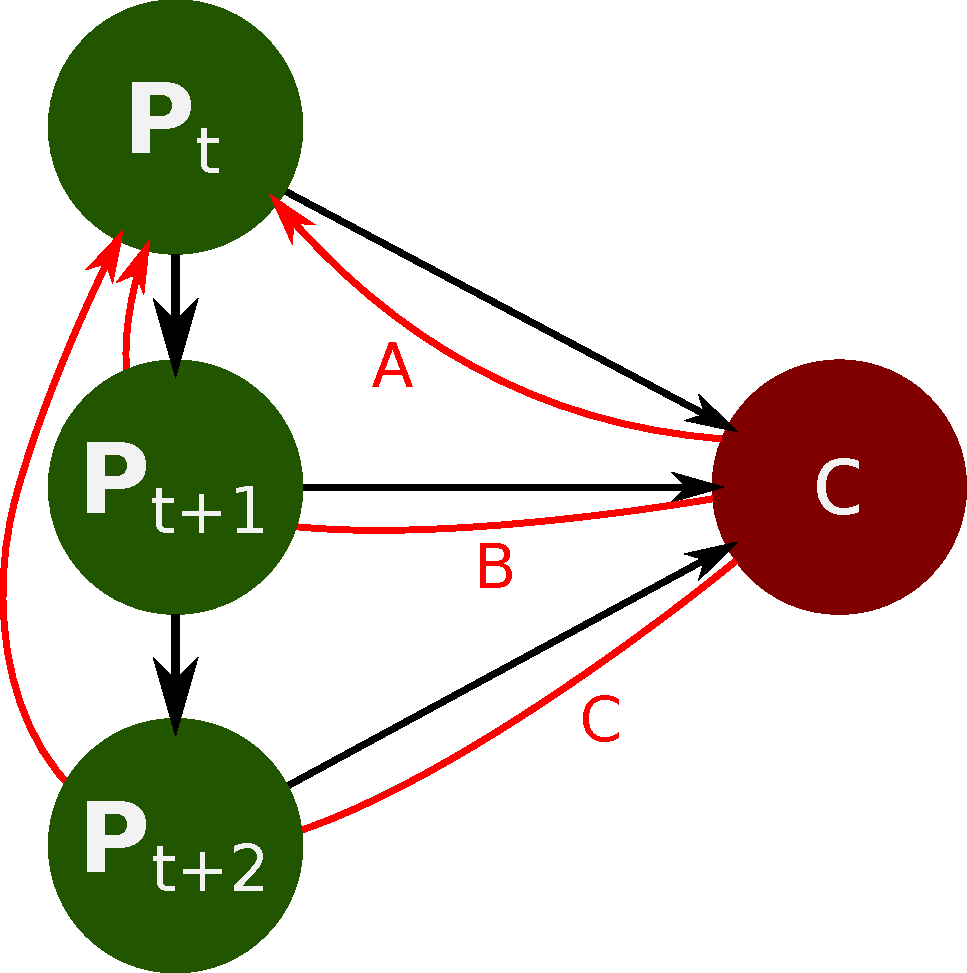
\includegraphics[width=0.3\textwidth]{diferenciando_custo_3_nos.pdf}
    \end{center}
    \caption{\DIFaddFL{Grafo da dependência (setas vermelhas) do custo $c$ em relação ao campo de pressão $P_t$. Num esquema de diferenças finitas de segunda ordem no tempo, três caminhos vão do custo ao campo de pressão em um tempo $t$: o caminho $A$ indica o erro gerado diretamente pela falta de fase entre o dado predito e o observado nos receptores no instante $t$; o caminho $B$ se refere ao erro propagado à pressão do instante seguinte ($t+1$) devido ao erro presente no instante $t$; e o caminho $C$ trata do erro causado à pressão em $t+2$ devido ao erro em $P_t$.}}
    \label{f:diferenciando_custo_3_nos}
  \end{figure}

  \DIFaddend \begin{equation} \label{e:parcial_custo_wrt_pressao_t_em_v}
    \frac{\partial c}{\partial \boldsymbol{\hat{P}}_t} \biggm\lvert_{\boldsymbol{V}} =
    \frac{\partial c}{\partial \boldsymbol{\hat{P}}_t} \biggm\lvert_{\boldsymbol{V}, \boldsymbol{P}_{t'\ne t}} + 
    \frac{\partial c}{\partial \boldsymbol{\hat{P}}_{t+1}} \biggm\lvert_{\boldsymbol{V}}
      \frac{\partial \boldsymbol{\hat{P}}_{t+1}}{\partial \boldsymbol{\hat{P}}_{t}} \biggm\lvert_{\boldsymbol{V}, \boldsymbol{P}_{t'\ne t, t+1}} +
    \frac{\partial c}{\partial \boldsymbol{\hat{P}}_{t+2}} \biggm\lvert_{\boldsymbol{V}}
      \frac{\partial \boldsymbol{\hat{P}}_{t+2}}{\partial \boldsymbol{\hat{P}}_{t}} \biggm\lvert_{\boldsymbol{V}, \boldsymbol{P}_{t'\ne t, t+2}}
    .
  \end{equation}

    O primeiro termo da equação (\ref{e:parcial_custo_wrt_pressao_t_em_v}) pode ser calculado com facilidade a partir da função custo:

  \begin{equation} \label{e:parcial_custo_wrt_pressao_t_em_v_e_t}
    \frac{\partial c}{\partial \boldsymbol{\hat{P}}_t} \biggm\lvert_{\boldsymbol{V}, \boldsymbol{P}_{t'\ne t}} =
    \frac{\partial}{\partial \boldsymbol{\hat{P}}_t}
      \left[\frac{1}{2}
        \sum \limits_{\vec{r} \in \mathcal{D}} \delta_{\vec{r}, \vec{r}_r}
        (\boldsymbol{\hat{P}}_t - y_t)
      \right]^2 \biggm\lvert_{\boldsymbol{V}, \boldsymbol{P}_{t'\ne t}} = 
      \delta_{\vec{r}, \vec{r}_r} (\boldsymbol{\hat{P}}_t - y_t) =
      e_t \boldsymbol{\delta}_{\vec{r}, \vec{r}_r}
    ,
  \end{equation}

  \noindent ou seja, seu valor é a amplitude do resíduo entre o dado modelado e o observado na posição do receptor, $e_t$. As equações (\ref{e:parcial_pressao_t_mais_1_wrt_pressao_t}), (\ref{e:parcial_pressao_t_mais_2_wrt_pressao_t}) e (\ref{e:parcial_pressao_t_wrt_velocidade}) podem ser calculadas a partir de (\ref{e:fdm_rnn_cell}).


  \begin{equation} \label{e:parcial_pressao_t_mais_1_wrt_pressao_t}
    \frac{\partial \boldsymbol{\hat{P}}_{t+1}}{\partial \boldsymbol{\hat{P}}_t} \biggm\lvert_{\boldsymbol{V}, \boldsymbol{P}_{t'\ne t, t+1}} =
    \boldsymbol{V}^2 {\Delta t}^2 \nabla^2 + 2
  \end{equation}

  \begin{equation} \label{e:parcial_pressao_t_mais_2_wrt_pressao_t}
    \frac{\partial \boldsymbol{\hat{P}}_{t+2}}{\partial \boldsymbol{\hat{P}}_t} \biggm\lvert_{\boldsymbol{V}, \boldsymbol{P}_{t'\ne t, t+2}} =
    -1
  \end{equation}

  \begin{equation} \label{e:parcial_pressao_t_wrt_velocidade}
    \frac{\partial \boldsymbol{\hat{P}}_{t}}{\partial \boldsymbol{V}} \biggm\lvert_{\boldsymbol{P}_{t'\ne t}} =
    2 \boldsymbol{V} {\Delta t}^2 (\nabla^2 \boldsymbol{\hat{P}}_{t-1} + 2 s_{t-1} \boldsymbol{\delta}_{\vec{r}, \vec{r}_s})
  \end{equation}

  \DIFdelbegin \DIFdel{Substituíndo }\DIFdelend \DIFaddbegin \DIFadd{Substituindo }\DIFaddend (\ref{e:parcial_custo_wrt_pressao_t_em_v}) em (\DIFdelbegin \DIFdel{\ref{e:parcial_custo_wrt_pressao_t_em_v}}\DIFdelend \DIFaddbegin \DIFadd{\ref{e:parcial_custo_wrt_velocidade}}\DIFaddend ), temos:

  \begin{equation} \label{e:parcial_custo_wrt_velocidade_subs_1}
    \begin{split}
      \frac{\partial c}{\partial \boldsymbol{V}} =
        \sum \limits_{t=1}^T \biggm( &
          \frac{\partial c}{\partial \boldsymbol{\hat{P}}_t} \biggm\lvert_{\boldsymbol{V}, \boldsymbol{P}_{t'\ne t}} \\
        & + \frac{\partial c}{\partial \boldsymbol{\hat{P}}_{t+1}} \biggm\lvert_{\boldsymbol{V}}
                \frac{\partial \boldsymbol{\hat{P}}_{t+1}}{\partial \boldsymbol{\hat{P}}_{t}} \biggm\lvert_{\boldsymbol{V}, \boldsymbol{P}_{t'\ne t, t+1}} \\
        & + \frac{\partial c}{\partial \boldsymbol{\hat{P}}_{t+2}} \biggm\lvert_{\boldsymbol{V}}
                \frac{\partial \boldsymbol{\hat{P}}_{t+2}}{\partial \boldsymbol{\hat{P}}_{t}} \biggm\lvert_{\boldsymbol{V}, \boldsymbol{P}_{t'\ne t, t+2}}
        \biggm)
        2 \boldsymbol{V} {\Delta t}^2 (\nabla^2 \boldsymbol{\hat{P}}_{t-1} + 2 s_{t-1} \boldsymbol{\delta}_{\vec{r}, \vec{r}_s})
    \end{split}
    .
  \end{equation}

  \DIFdelbegin \DIFdel{Substituíndo }\DIFdelend \DIFaddbegin \DIFadd{Sobrepondo }\DIFaddend então (\DIFdelbegin \DIFdel{\ref{e:parcial_custo_wrt_pressao_t_em_v}}\DIFdelend \DIFaddbegin \DIFadd{\ref{e:parcial_custo_wrt_pressao_t_em_v_e_t}}\DIFaddend ), (\ref{e:parcial_pressao_t_mais_1_wrt_pressao_t}) e (\ref{e:parcial_pressao_t_mais_2_wrt_pressao_t}) \DIFdelbegin \DIFdel{em }\DIFdelend \DIFaddbegin \DIFadd{a }\DIFaddend (\ref{e:parcial_custo_wrt_velocidade_subs_1}), conseguimos:

  \begin{equation} \label{e:parcial_custo_wrt_velocidade_subs_2}
    \begin{split}
      \frac{\partial c}{\partial \boldsymbol{V}} = 
      \sum \limits_{t=1}^T \biggm( &
        e_t \boldsymbol{\delta}_{\vec{r}, \vec{r}_r}
        + (\boldsymbol{V}^2 {\Delta t}^2 \nabla^2 + 2) \frac{\partial c}{\partial \boldsymbol{\hat{P}}_{t+1}} \biggm\lvert_{\boldsymbol{V}}
        - \frac{\partial \boldsymbol{\hat{P}}_{t+2}}{\partial \boldsymbol{\hat{P}}_{t}} \biggm\lvert_{\boldsymbol{V}, \boldsymbol{P}_{t'\ne t, t+2}}
      \biggm) \\
      & 2 \boldsymbol{V} {\Delta t}^2 (\nabla^2 \boldsymbol{\hat{P}}_{t-1} + 2 s_{t-1} \boldsymbol{\delta}_{\vec{r}, \vec{r}_s})
    \end{split}
    ,
  \end{equation}

  Podemos rearrumar os termos de (\DIFdelbegin \DIFdel{\ref{e:parcial_custo_wrt_velocidade_subs_1}}\DIFdelend \DIFaddbegin \DIFadd{\ref{e:parcial_custo_wrt_velocidade_subs_2}}\DIFaddend ) da seguinte maneira:

  \begin{equation} \label{e:parcial_custo_wrt_velocidade_rearrumado_2}
    \DIFdelbegin %DIFDELCMD < \begin{split}
%DIFDELCMD <       \frac{\partial c}{\partial \boldsymbol{V}} =
%DIFDELCMD <       \sum \limits_{t=1}^T \biggm(
%DIFDELCMD <         & \boldsymbol{V}^2 {\Delta t}^2 \left(
%DIFDELCMD <           \nabla^2 \frac{\partial c}{\partial \boldsymbol{\hat{P}}_{t+1}} \biggm\lvert_{\boldsymbol{V}} + \frac{e_t \boldsymbol{\delta}_{\vec{r}, \vec{r}_r}}{\boldsymbol{V}^2 {\Delta t}^2}
%DIFDELCMD <         \right) + 2 \frac{\partial c}{\partial \boldsymbol{\hat{P}}_{t+1}} \biggm\lvert_{\boldsymbol{V}}) -
%DIFDELCMD <         \frac{\partial c}{\partial \boldsymbol{\hat{P}}_{t+2}} \biggm\lvert_{\boldsymbol{V}}
%DIFDELCMD <       \biggm) \\
%DIFDELCMD <       & 2 \boldsymbol{V} {\Delta t}^2 (\nabla^2 \boldsymbol{\hat{P}}_{t-1} + 2 s_{t-1} \boldsymbol{\delta}_{\vec{r}, \vec{r}_s})
%DIFDELCMD <     \end{split}%%%
\DIFdelend \DIFaddbegin \begin{split}
      \frac{\partial c}{\partial \boldsymbol{V}} =
      \sum \limits_{t=1}^T \biggm(
        & \boldsymbol{V}^2 {\Delta t}^2 \left(
          \nabla^2 \frac{\partial c}{\partial \boldsymbol{\hat{P}}_{t+1}} \biggm\lvert_{\boldsymbol{V}} + \frac{e_t \boldsymbol{\delta}_{\vec{r}, \vec{r}_r}}{\boldsymbol{V}^2 {\Delta t}^2}
        \right) + 2 \frac{\partial c}{\partial \boldsymbol{\hat{P}}_{t+1}} \biggm\lvert_{\boldsymbol{V}} -
        \frac{\partial c}{\partial \boldsymbol{\hat{P}}_{t+2}} \biggm\lvert_{\boldsymbol{V}}
      \biggm) \\
      & 2 \boldsymbol{V} {\Delta t}^2 (\nabla^2 \boldsymbol{\hat{P}}_{t-1} + 2 s_{t-1} \boldsymbol{\delta}_{\vec{r}, \vec{r}_s})
    \end{split}\DIFaddend 
    .
  \end{equation}

  \noindent \DIFdelbegin \DIFdel{Podemos enxergar }\DIFdelend \DIFaddbegin \DIFadd{Enxergamos }\DIFaddend em (\ref{e:parcial_custo_wrt_velocidade_rearrumado_2}) o padrão da função de modelagem $f$ no primeiro fator do somatório:

  \begin{equation} \label{e:parcial_custo_wrt_velocidade_propagacao_reversa}
    \frac{\partial c}{\partial \boldsymbol{V}} =
    \sum \limits_{t=1}^T
    f\left(\boldsymbol{V},
      \frac{\partial c}{\partial \boldsymbol{\hat{P}}_{t+2}} \biggm\lvert_{\boldsymbol{V}}, \frac{\partial c}{\partial \boldsymbol{\hat{P}}_{t+1}} \biggm\lvert_{\boldsymbol{V}}, \frac{e_t \boldsymbol{\delta}_{\vec{r}, \vec{r}_r}}{\boldsymbol{V} {\Delta t}^2}
    \right)
    2 \boldsymbol{V} {\Delta t}^2 (\nabla^2 \boldsymbol{\hat{P}}_{t-1} + 2 s_{t-1} \boldsymbol{\delta}_{\vec{r}, \vec{r}_s})
    .
  \end{equation}

  Já no segundo fator de (\ref{e:parcial_custo_wrt_velocidade_rearrumado_2}) podemos ver a segunda derivada do campo primário, uma vez que:

  \begin{equation} \label{e:de_volta_das_diferencas_finitas_para_segunda_derivada_analitica}
    \frac{\boldsymbol{\hat{P}}_t - 2 \boldsymbol{\hat{P}}_{t-1} + \boldsymbol{\hat{P}}_{t-2}}{{\Delta t}^2}
    \approx
    \boldsymbol{\ddot{\hat{P}}}_{t-1}
    =
    \boldsymbol{V}^2 (\nabla^2 \boldsymbol{\hat{P}}_{t-1} + s_{t-1} \boldsymbol{\delta}_{\vec{r}, \vec{r}_s})
    ,
  \end{equation}

  \noindent e portanto,

  \begin{equation} \label{e:segundo_fator_vem_da_segunda_derivada_no_tempo}
    \nabla^2 \boldsymbol{\hat{P}}_{t-1} + s_{t-1} \boldsymbol{\delta}_{\vec{r}, \vec{r}_s}
    =
    \frac{\boldsymbol{\ddot{\hat{P}}}_{t-1}}{\boldsymbol{V}^2}
    .
  \end{equation}

  \noindent Ficamos então com (\ref{e:parcial_custo_wrt_velocidade_propagacao_reversa_com_dt}).

  \begin{equation} \label{e:parcial_custo_wrt_velocidade_propagacao_reversa_com_dt}
    \frac{\partial c}{\partial \boldsymbol{V}} =
    \sum \limits_{t=1}^T
    f\left(\boldsymbol{V},
      \frac{\partial c}{\partial \boldsymbol{\hat{P}}_{t+2}} \biggm\lvert_{\boldsymbol{V}}, \frac{\partial c}{\partial \boldsymbol{\hat{P}}_{t+1}} \biggm\lvert_{\boldsymbol{V}}, \frac{e_t \boldsymbol{\delta}_{\vec{r}, \vec{r}_r}}{\boldsymbol{V} {\Delta t}^2}
    \right)
    \frac{2}{\boldsymbol{V}} {\Delta t}^2 \boldsymbol{\ddot{\hat{P}}}_{t-1}
  \end{equation}

  Dada a linearidade da equação da onda a tempos pequenos, podemos por para fora os fatores do terceiro argumento de $f$ e mover as variáveis independentes do tempo para fora do somatório para obter (\ref{e:parcial_custo_wrt_velocidade_propagacao_reversa_final}).

  \begin{equation} \label{e:parcial_custo_wrt_velocidade_propagacao_reversa_final}
    \boldsymbol{\nabla} c \equiv \frac{\partial c}{\partial \boldsymbol{V}} =
    \frac{2}{\boldsymbol{V}^3}
    \sum \limits_{t=1}^T
    f\left(\boldsymbol{V},
      \frac{\partial c}{\partial \boldsymbol{\hat{P}}_{t+2}} \biggm\lvert_{\boldsymbol{V}}, \frac{\partial c}{\partial \boldsymbol{\hat{P}}_{t+1}} \biggm\lvert_{\boldsymbol{V}}, e_t \boldsymbol{\delta}_{\vec{r}, \vec{r}_r}
    \right)
    \boldsymbol{\ddot{\hat{P}}}_{t-1}
  \end{equation}

  A equação (\ref{e:parcial_custo_wrt_velocidade_propagacao_reversa_final}) é exatamente a discretização da solução para o gradiente da função custo do erro quadrático dada pelo método adjunto: \DIFdelbegin \DIFdel{A }\DIFdelend \DIFaddbegin \DIFadd{a }\DIFaddend função $f$ está propagando o resíduo $e_t$ reversamente no tempo --- a extrapolação vai \DIFdelbegin \DIFdel{dos }\DIFdelend \DIFaddbegin \DIFadd{do }\DIFaddend tempo $t+2$ para $t+1$ para \DIFaddbegin \DIFadd{sem seguida }\DIFaddend produzir $t$ --- a partir da posição do receptor, $\vec{r}_r$. O resultado desta operação é o campo adjunto do método adjunto, $\lambda$, que é multiplicado pela segunda derivada no tempo do campo modelado. Este resultado \DIFdelbegin \DIFdel{, com }\DIFdelend \DIFaddbegin \DIFadd{para }\DIFaddend uma única fonte é \DIFdelbegin \DIFdel{extendido }\DIFdelend \DIFaddbegin \DIFadd{estendido }\DIFaddend a mais receptores somando suas contribuições na função custo, e a mais fontes, ao realizar a modelagem direta com mais fontes \shortcite{sun2019deep}.


\DIFdelbegin %DIFDELCMD < \appendix{Receita para o treinamento estocástico de um modelo supervisionado ou não-supervisionado} %%%
\DIFdelend \DIFaddbegin \appendix{Receita para o treinamento estocástico de um modelo supervisionado} \DIFaddend \label{a:guia_treinamento}

    Durante os estudos práticos \DIFdelbegin \DIFdel{, o }\DIFdelend \DIFaddbegin \DIFadd{de treinamento de modelos supervisionados, tais como o do modelo de regressão logística, a inversão de forma completa da onda implementada, o }\DIFaddend autor verificou um padrão estrutural \DIFdelbegin \DIFdel{durante }\DIFdelend \DIFaddbegin \DIFadd{para }\DIFaddend a implementação de códigos de otimização em um paradigma fortemente funcional, de \DIFdelbegin \DIFdel{forma que os resultados são }\DIFdelend \DIFaddbegin \DIFadd{maneira que os códigos se tornam }\DIFaddend mais facilmente reutilizáveis. Tal padrão pode ser \DIFaddbegin \DIFadd{utilizado para o desenvolvimento de qualquer modelo estatístico supervisionado ou de qualquer inversão geofísica, e é }\DIFaddend sumarizado em três fases:

    \begin{enumerate}
      \item Fase de \emph{criação do modelo}, a qual envolve:
        \begin{enumerate}
          \item Definição do(s) modelo(s) direto(s) --- durante esta etapa deve-se implementar os problemas diretos necessários que levarão uma sequência de parâmetros $\{W_s\}$ e uma matriz de amostras observadas $\boldsymbol{X}$ a uma matriz de predições $\boldsymbol{\hat{Y}}$. Este processo muitas vezes inclui o primeiro desenvolvimento de modelos que levam uma única amostra $\vec{x}$ à sua predição $\vec{y}$.
          \item Em caso de otimização conjunta de dois ou mais modelos diretos deve-se implementar um modelo amarrador que retorna as saídas finais que podem ser utilizadas no treinamento.
          \item Em caso de regularização dos parâmetros durante treinamento, pode ser desejável adicionar os parâmetros como saídas do modelo final utilizado no treinamento.
        \end{enumerate}
      \item Fase de \emph{preparação do treinamento}, que nos termos aqui descritos só faz sentido para numa abordagem funcional. Caso se utilize uma abordagem imperativa, pular à próxima fase. Suas etapas são:
        \begin{enumerate}
          \item Preparação dos dados a serem utilizados no treinamento, incluíndo a estrutura de observações $\boldsymbol{X}$ e estrutura \DIFdelbegin \DIFdel{com }\DIFdelend \DIFaddbegin \DIFadd{de }\DIFaddend seus alvos $\boldsymbol{Y}$ caso aplicável.
          \item Preparação do método de validação (\textit{i.e.}, \textit{holdout}, \textit{k-fold}).
          \item Definição da função custo de erro médio $C(\{\boldsymbol{W}_s\}, \boldsymbol{X}_b, \boldsymbol{Y}_b)$\DIFdelbegin \DIFdel{(lote de observações e de alvos)}\DIFdelend , que toma \DIFdelbegin \DIFdel{um lote de predições e }\DIFdelend \DIFaddbegin \DIFadd{os parâmetros, o lote de dados e seus alvos, e }\DIFaddend retorna um valor em $\mathcal{R}$. Frequentemente inclui-se aqui a definição anterior do custo calculado sobre uma única amostra, $c_n(\{\boldsymbol{W}_s\}, \vec{x}, \vec{y})$.
          \item Opcional: pode-se definir uma função para calcular outras métricas úteis \DIFaddbegin \DIFadd{(}\textit{\DIFadd{i.e.}}\DIFadd{, precisão, acurácia, além do custo) }\DIFaddend a partir de um lote de predições, $\boldsymbol{\hat{Y}}$, e seus valores verdadeiros, $\boldsymbol{Y}$.
          \item Implementação do funcional que toma um modelo, uma função custo médio e, se aplicável, parâmetros da regularização de parâmetros utilizada (\textit{i.e.}\DIFaddbegin \DIFadd{, }\DIFaddend coeficiente do termo de esparsidade dos parâmetros na função custo), e define uma função para calcular o custo $C$ e o gradiente do custo $\nabla C$ deste modelo com relação aos parâmetros dados, \DIFaddbegin \DIFadd{por diferenciação automática, }\DIFaddend partindo deles e de um lote de dados composto por $\boldsymbol{X}_b$ e $\boldsymbol{Y}_b$, caso aplicável. Eventualmente pode ser interessante retornar também nesta função as métricas avaliadas em treinamento por meio de uma função previamente definida, desde que isto não adicione complexidade significativa ao algoritmo de treinamento e haja tempo o suficiente para tal.
          \item Criação de um funcional que toma o modelo e uma função custo para produzir uma função que toma parâmetros e um lote de dados, e retorna suas predições, custo e outras métricas, caso definidas.
          \item Criação de um funcional que toma uma função custo e retorna uma função que treina o modelo por uma época. Para tal, esta função deve recebe um otimizador (\textit{i.e.}, SGD)  com suas variáveis de estado, o lote total de dados a ser utilizado no treinamento, o número de amostras a ser utilizada no treinamento estocástico, e se desejado, uma chave para realizar acumulação de gradientes ou não. A função gerada retornará em cada aplicação pelo menos os parâmetros atualizados após uma época, as novas variáveis de estado do otimizador e as métricas médias obtidas nesta mesma época.
        \end{enumerate}
      \item Fase de \emph{treinamento}, a qual inclui:
        \begin{enumerate}
          \item A geração das funções --- \DIFdelbegin \DIFdel{caso na abordagem funcional, utilizar }\DIFdelend \DIFaddbegin \DIFadd{aplicar }\DIFaddend os funcionais implementados no passo anterior:
            \begin{enumerate}
              \item de treinamento de uma época em função de um otimizador, dados de treinamento, número de amostras por lote e, se desejado, uma opção para acumular gradientes ou não;
              \item de avalização das métricas do modelo.
            \end{enumerate}
          \item Inicializar o otimizador escolhido (\textit{i.e.}, SGD).
          \item Definir uma condição de parada, como a descrita na Seção \ref{s:interrupcao_precoce} ou número máximo de épocas --- não recomendado, pois este parâmetro é difícil de ser escolhido.
          \item Definir uma estrutura de dados para o guardar um histórico de métricas de treinamento.
          \item Criar o laço de treinamento, que tipicamente envolve:
            \begin{enumerate}
              \item treinar uma época;
              \item imprimir \DIFaddbegin \DIFadd{o }\DIFaddend estado do treinamento (\textit{i.e.}, época e valor do custo \DIFaddbegin \DIFadd{atual}\DIFaddend );
              \item atualizar histórico com as métricas atuais;
              \item criar \textit{checkpoint} do modelo --- isto é, salvar seus parâmetros em uma estrutura (tipicamente em disco);
              \item atualizar da condição de parada a partir da métrica avaliada e dos parâmetros atuais;
              \item verificar se a condição de parada retorna verdadeiro. Caso positivo, recuperar \DIFaddbegin \DIFadd{o }\DIFaddend \textit{checkpoint} dos melhores parâmetros do modelo e finalizar treinamento.
            \end{enumerate}
          \item Visualizar saídas do modelo.
          \item Visualizar histórico de métricas salvo\DIFaddbegin \DIFadd{, verificar condições de viés e variância para considerar situações de subajuste ou sobreajuste}\DIFaddend .
          \item Salvar parâmetros do modelo treinado.
        \end{enumerate}
    \end{enumerate}

    Além dos passos apontados acima, vale ressaltar que os parâmetros do otimizador, como a taxa de aprendizado, ou os parâmetros da função custo, como os relacionados à regularização do modelo, devem ser testados para que possam ser \DIFdelbegin \DIFdel{escolhidos}\DIFdelend \DIFaddbegin \DIFadd{definidos}\DIFaddend .


\appendix{Transformação \textit{one-hot}} \label{a:one_hot}

  A transformação ou codificação \textit{one-hot} consiste numa simples transformação rótulos inteiros em probabilidades de pertencimento a cada classe. Assim, se um problema considera que amostras podem pertencer a três classes, enumeradas de 1 a 3, o rótulo 1 se torna $[1.0,\ 0.0,\ 0.0]^\top$, o rótulo 2 se torna $[0.0,\ 1.0,\ 0.0]^\top$, e o rótulo 3 se torna $[0.0,\ 0.0,\ 1.0]^\top$, onde cada linha $i$ destes vetores diz respeito à probabilidade de pertencimento da amostra à classe $i$.

  Geralmente esta aplicação é realizada em massa para um vetor de $N$ rótulos, $\vec{r}$, o qual é associado a uma matriz de observações das $N$ amostras $\boldsymbol{X}_{N\times M}$. O resultado deste processo é uma matriz $\boldsymbol{Y}$ cujas linhas são dadas pela transposta da transformação \textit{one-hot} das linhas em $\vec{r}$. Isto pode ser verificado no caso abaixo:

  \begin{equation}
    \text{one-hot} \left(
    \begin{bmatrix}
      1 \\
      2 \\
      2 \\
      3
    \end{bmatrix} \right)
    =
    \begin{bmatrix}
      1.0 & 0.0 & 0.0 \\
      0.0 & 1.0 & 0.0 \\
      0.0 & 1.0 & 0.0 \\
      0.0 & 0.0 & 1.0 \\
    \end{bmatrix}
    .
  \end{equation}

  A transformação one-hot pode ser invertida aplicando a função de argumento do máximo (argmax) em cada linha da matriz transformada. Esta função retorna o índice do elemento com maior valor do vetor aplicado:

  \begin{equation}
    \text{argmax} \left(
    \begin{bmatrix}
      1.0 & 0.0 & 0.0 \\
      0.0 & 1.0 & 0.0 \\
      0.0 & 1.0 & 0.0 \\
      0.0 & 0.0 & 1.0 \\
    \end{bmatrix} \right)
    =
    \begin{bmatrix}
      1 \\
      2 \\
      2 \\
      3
    \end{bmatrix}
    .
  \end{equation}

\appendix{Código para diferenciação automática direta} \label{a:autodiff_direta}

  Este código implementa um ambiente de diferenciação automática direta na linguagem Python 3.9 de forma simples, sem o uso de bibliotecas externas. Ele não deve ser considerado em aplicações com alta demanda computacional, uma vez que foi escrito com fins didáticos.

  \lstinputlisting[language=Python]{code/forward_mode.py}


\appendix{Código para diferenciação automática reversa} \label{a:autodiff_reversa}

  Este código implementa um ambiente de diferenciação automática reversa na linguagem Python 3.9 de forma simples, sem o uso de bibliotecas externas. Ele não deve ser considerado em aplicações com alta demanda computacional, uma vez que foi escrito com fins didáticos. Uma aplicação desta implementação pode ser vista no Apêndice \ref{a:treinamento_mlp}, onde uma rede neural tipo perceptron multicamadas é treinada.

  \lstinputlisting[language=Python]{code/reverse_mode.py}


\appendix{Código para treinamento de rede neural MLP usando diferenciação automática} \label{a:treinamento_mlp}

  Este código escrito em Python 3.9 importa o código presente no Apêndice \ref{a:autodiff_reversa} para realizar o cálculo de gradientes por meio da diferenciação automática reversa, qual é utilizado no treinamento de uma rede perceptron multicamadas sem o uso de bibliotecas externas. O algoritmo de otimização utilizado é o SGD.

  \lstinputlisting[language=Python]{code/mlp.py}

%%%%%%%%%%%%%%%%%%%%%%%%%%%%%%%%%%%%%%%%%%%%%%%%%%%%%%%%%%%%%%%%%%%
%                                                                 %
%                           BIBLIOGRAFIA                          %
%                                                                 %
%%%%%%%%%%%%%%%%%%%%%%%%%%%%%%%%%%%%%%%%%%%%%%%%%%%%%%%%%%%%%%%%%%%
% O exemplo abaixo é o recomendado pois utiliza o bibtex que
% assegura uma lista de referências completa e sem falta.
%
% Entretanto, para aqueles que continuam usando a montagem manual,
% este arquivo deve iniciar-se com
%	\chapter*{Referências Bibliográficas}
%	\addcontentsline{toc}{chapter}{Referências Bibliográficas}
%	\markboth{Referências Bibliográficas}{Referências Bibliográficas}
% 
 
\selectlanguage{brazil}
\bibliographystyle{pppgbib}
%\bibliographystyle{plainnat}

% Note que o argumento do comando \bibliography é longo e, por isso,
% foi dividido em diversas linhas. A presença do % é fundamental 
% para eliminar o "fim de linha"
%\bibliography{bib-article,bib-book,bib-proceeding,bib-collection,bib-thesis,bib-master,bib-tcc,bib-report,bib-manual,bib-misc}
\bibliography{mybib}

%%%%%%%%%%%%%%%%%%%%%%%%%%%%%%%%%%%%%%%%%%%%%%%%%%%%%%%%%%%%%%%%%%%
%                                                                 %
%                            ANEXOS                               %
%                                                                 %
% O apendice tem uma relacao muito mais forte com o corpo da      %
% tese do que o anexo.                                            %
%                                                                 %
% Por exemplo, podemos utilizar o apendice para a demonstracao    %
% de uma longa passagem matematica que nao contribui diretamente  %
% ao entendimento do texto principal.                             %
%                                                                 %
% O anexo seria dedicado aquelas outras informacoes, principal-   %
% mente aquelas oriundas de outros autores. Tambem podemos        %
% lancar no anexo os programas de computadores                    %
%                                                                 %
% Observe o ambiente verbatin utilizado a seguir                  %
%                                                                 %
%%%%%%%%%%%%%%%%%%%%%%%%%%%%%%%%%%%%%%%%%%%%%%%%%%%%%%%%%%%%%%%%%%%



%%%%%%%%%%%%%%%%%%%%%%%%%%%%%%%%%%%%%%%%%%%%%%%%%%%%%%%%%%%%%%%%%%%%%%%%
%%%%%%%%%%%%%%%%%%%%%%%%%%%%%%%%%%%%%%%%%%%%%%%%%%%%%%%%%%%%%%%%%%%%%%%%
%%%%%%%%%%%%%%%%%%%%%%%%%%%%%%%%%%%%%%%%%%%%%%%%%%%%%%%%%%%%%%%%%%%%%%%%
%%%%%%%%%%%%%%%%%%%%%%%%%%%%%%%%%%%%%%%%%%%%%%%%%%%%%%%%%%%%%%%%%%%%%%%%
%******************************************************************
% 
%                         SEGUNDO ANEXO
%
%******************************************************************
%\annex{Diferença entre apêndice e anexo}
% 
%
%Segundo a NBR 14724 de dezembro de 2005, a diferença primordial entre Anexo e Apêndice é que o Anexo é um texto ou documento não elaborado pelo autor do Trabalho Científico (TC) (monografia, tese, etc.) e o Apêndice é um texto ou documento elaborado pelo autor do TC, ou seja, se foi necessário você criar uma entrevista, um relatório, ou qualquer documento com o escopo de complementar sua argumentação, deve-se utilizar o termo Apêndice e não Anexo. 
%
%\noindent{\small\tt http://www.tudosobremonografia.com/2011/01/diferenca-entre-anexo-e-apendice.html}
%

%\capitulo{Cronograma}
%\chapter*{Cronograma}
%\addcontentsline{toc}{chapter}{Cronograma}



%\begin{sidewaystable}
\newcommand{\marca}{\rule{0.8cm}{.2cm}}
\begin{center}
  \begin{tabular}{c|cccccccc}\hline
    \multirow{2}{*}{Etapa}	&\multicolumn{8}{c}{Mês}\\\cline{2-9}
    			  	&01&02&03&04&05&06&07&08\\\hline
%%%%%%%%%%%%%%%%%%%%%%	&\marca &\marca &\marca &\marca &\marca &\marca &\marca &\marca \\ 	
Pesquisa Bibliográfica	&\marca &\marca &\marca &\marca &\marca &\marca &\marca &       \\ 	
Estudo dos programas	&       &\marca &\marca &       &       &       &       &       \\ 	
Coleta de dados		&       &       &\marca &\marca &       &       &       &       \\ 	
Relatório		&       &       &       &\marca &       &       &       &       \\ 	
Processamento dos dados	&       &       &       &       &\marca &\marca &       &       \\
Interpretação		&       &       &       &       &	&\marca &\marca &\marca \\
Preparação do TFG	&       &       &       &       &       &\marca &\marca &\marca \\
Apresentação		&       &       &       &       &       &       &       &\marca \\
    \hline
  \end{tabular}
\end{center}
%\end{sidewaystable}


%\begin{tabular}{c|>{\centering}p{15ex}>{\centering}p{15ex}c}\hline

 % relatório
%%%%%%%%%%%%%%%%%%%%%%%%%%%%%%%%%%%%%%%%%%%%%%%%%%%%%%%%%%%%%%%%%%%%%%%%%%%%%%%%%
%
%           CAPITULO EXPERIMENTAL
%
%%%%%%%%%%%%%%%%%%%%%%%%%%%%%%%%%%%%%%%%%%%%%%%%%%%%%%%%%%%%%%%%%%%%%%%%%%%%%%%%

\capitulo{Avaliação do Orientador}
%\chapter*{Observações do Orientador}
%\addcontentsline{toc}{chapter}{Observações do Orientador}

Em relação ao orientando \authorname, declaro
\begin{itemize}
  \item nota 10 (dez) por sua atividade na disciplina GEO213 -- Trabalho Final de Graduação, e
  \item frequência integral (100~\%).
\end{itemize}	


\vspace{1cm}
\begin{center}
%	Prof. Grande Orientador\\
%	Orientador
  \baselineskip=2cm
	\Orientador
\end{center}

%

 % relatório
\end{document}
